\documentclass[11pt]{report}
\usepackage{amssymb}
\usepackage{amsmath}
\usepackage{amsthm}
\usepackage{url}
\usepackage{graphicx,geometry,color}
\usepackage{makeidx}
\usepackage{alltt}
\usepackage[hyperfootnotes=false]{hyperref}
\usepackage[all]{xy}
\usepackage{fancyhdr}
\usepackage{pdfpages}
\newcommand{\cpsa}{\textsc{cpsa}}
\newcommand{\version}{4.4.3}
\newcommand{\cpsacopying}{\begingroup
  \renewcommand{\thefootnote}{}\footnotetext{{\copyright} 2010 The
    MITRE Corporation.  Permission to copy without fee all or part of
    this material is granted provided that the copies are not made or
    distributed for direct commercial advantage, this copyright notice
    and the title of the publication and its date appear, and notice
    in given that copying is by permission of The MITRE
    Corporation.}\endgroup}
\newcommand{\pov}{\textsc{pov}}
\newcommand{\cow}{\textsc{cow}}
\newcommand{\cn}[1]{\ensuremath{\operatorname{\mathsf{#1}}}}
\newcommand{\dom}[1]{\ensuremath{\operatorname{\mathbf{#1}}}}
\newcommand{\fn}[1]{\ensuremath{\operatorname{\mathit{#1}}}}
\newcommand{\seq}[1]{\ensuremath{\langle#1\rangle}}
\newcommand{\enc}[2]{\ensuremath{\{\!|#1|\!\}_{#2}}}
\newcommand{\hash}[1]{\ensuremath{\##1}}
\newcommand{\comp}[2]{{\mathord{#1}}\circ{\mathord{#2}}}
\newcommand{\sembrack}[1]{[\![#1]\!]}
\newcommand{\semfn}[1]{\mathcal{#1}}
\newcommand{\sem}[2]{\semfn{#1}\sembrack{#2}}
\newcommand{\mcsu}{\ensuremath{\mathcal{C}}}
\newcommand{\probs}{\ensuremath{\mathcal{E}}}
\newcommand{\srt}[1]{\ensuremath{\mathsf{#1}}}
\newcommand{\eqq}{\stackrel{?}{=}}
\newcommand{\inbnd}{\mathord -}
\newcommand{\outbnd}{\mathord +}
\newcommand{\nat}{\mathbb{N}}
\newcommand{\all}[1]{\mathop{\forall#1}}
\newcommand{\some}[1]{\mathop{\exists#1}}
\newcommand{\baseterms}{\mathbb{B}}
\newcommand{\cons}{\mathbin{::}}
\newcommand{\ith}{\imath^\mathrm{th}}
\newcommand{\jth}{\jmath^\mathrm{th}}
\newcommand{\append}{\mathbin{{}^\smallfrown}}
\newcommand{\prefix}[2]{#1\dagger#2}
\newcommand{\orig}{\mathcal{O}}
\newcommand{\gain}{\mathcal{G}}
%\newcommand{\pow}[1]{\mathcal{P}(#1)}
%\newcommand{\pow}[1]{\wp(#1)}
\newcommand{\pow}[1]{2^{#1}}
\newcommand{\termat}{\mathbin{@}}
\newcommand{\idsigma}{\sigma_{\mathrm{id}}}
\newcommand{\idphi}{\phi_{\mathrm{id}}}
\newcommand{\kprec}[1]{\mathbin{\prec_{#1}}}
\newcommand{\terms}{\ensuremath{\mathcal{T}}}
\newcommand{\alg}[1]{\ensuremath{\mathfrak#1}}
\newcommand{\ops}[1]{\ensuremath{\mathbb#1}}
\newcommand{\bundle}{\ensuremath{\mathcal{B}}}
\newcommand{\der}[3]{\ensuremath{\dctx{#2}{#3}\vdash#1}}
\newcommand{\dctx}[2]{\ensuremath{#1:#2}}
\newcommand{\flow}[3]{\ensuremath{#1,#2\rhd#3}}
\newcommand{\infer}[2]{\begin{array}{c}#1\\\hline#2\end{array}}
\hyphenation{pre-skel-e-ton}
\newcommand{\homomorphism}[1]{\stackrel{#1}{\longmapsto}}
\newcommand{\reduction}[1]{\stackrel{#1}{\longrightarrow}}
\newcommand{\longtwoheadrightarrow}{\relax
\smash{\relbar\joinrel\twoheadrightarrow}\vphantom\rightarrow}
\newcommand{\setreduction}[1]{\stackrel{#1}{\longtwoheadrightarrow}}
\newcommand{\uniqat}{\mbox{\sf uniq-at}}
\newcommand{\strprec}{\mbox{\sf str-prec}}


\newif\ifpubrel
%\pubreltrue
\pubrelfalse

\fancypagestyle{title}{%
  \fancyhf{}%
  \renewcommand\headrulewidth{0pt}%
  \fancyhead[L]{Approved for Public Release; Distribution Unlimited. Case Number 15-3120.}%
  \fancyfoot[C]{This technical data was produced for the
    U.S. Government\\ under Contract. No. W15P7T-13-C-A802, and is\\
    subject to the Rights in Technical Data-Noncommercial Items clause\\
    at DFARS 252.227-7013 (FEB 2012)\\
\copyright 2016 The MITRE Corporation. ALL RIGHTS RESERVED.}%
}

\pagestyle{plain}

\makeindex

\title{The Cryptographic Protocol Shapes Analyzer:\\ A Manual for CPSA
  4}
\author{Moses D.~Liskov\qquad John D.~Ramsdell\\Joshua D.~Guttman\qquad Paul D.~Rowe\\ \\
  {\Large The MITRE Corporation}\\ \\ CPSA Version \version}

\makeindex
\begin{document}

\ifpubrel
\thispagestyle{title}
\fi
\maketitle
\ifpubrel
\thispagestyle{title}
\fi
\pagenumbering{roman}
\cpsacopying

\tableofcontents

\listoffigures

\listoftables

\newpage
\pagenumbering{arabic}
\setcounter{page}{1}
\chapter{Introduction}
\label{ch:intro}

{\cpsa}, the Cryptographic Protocol Shapes Analyzer, is a software tool
designed to assist in the design and analysis of cryptographic protocols.
A cryptographic protocol is a specific pattern of interaction between
principals.  TLS and IKE are some examples of well-known cryptographic protocols.

The tool takes as input a protocol definition and a partial
description of an execution, each built within a particular formal
model by the user.  It attempts to produce descriptions of \emph{all}
possible executions of the protocol that complete the partial
description, consistent with the presence of a powerful network adversary
capable of diverting, altering, replaying, or dropping network messages.
Such an adversary may be able to manipulate honest participants into an
unexpected execution, breaking a secrecy or authentication property that
the protocol was intended to achieve.

Naturally, there are infinitely many possible executions of a useful
protocol, since different participants can run it with varying
parameters, and the participants can run it repeatedly.  However, for
many naturally occurring protocols, there are only finitely many of
these runs that are \emph{essentially} different.  Indeed, there are
frequently very few, often just one or two, even in cases where the
protocol is flawed.  We call these minimal, essentially different
executions the \emph{shapes} of the protocol.  Authentication and
secrecy properties are easy to ``read off'' from the shapes, as are
attacks and anomalies.

The analysis performed by {\cpsa} is done within a pure Dolev-Yao
model~\cite{DolevYao83}; as such, the analysis reveals only structural
flaws in the protocols it analyzes.  It cannot detect flaws in underlying
cryptographic algorithms or in actual implementations of protocol participants.

The purpose of this document is to provide the background required to
make effective use of the {\cpsa} software distribution.

\section{Recommended reading}

If you are new to {\cpsa}, it is recommended that you first read
Part~\ref{part:basic}, which is introductory in nature and presented
as a tutorial.  Chapter~\ref{ch:setup} discusses how to download,
install, and run the tool.  Chapter~\ref{ch:basic} begins the tutorial
describing how to use the tool, and Chapter~\ref{ch:algebra} describes
some of the more important additional features.

Readers, especially those without direct access to an experienced user
of the tool, are encouraged to attempt the ``explorations'' present
from Chapter~\ref{ch:basic} onwards.  The purpose of the explorations
is to give the reader experience in the use of the tool and a chance
to test his or her understanding of its features.  After reading
through the first part, you should be ready to attempt to use the tool
to analyze a protocol that interests you, whether it be an existing
protocol or one you need to design.

When you are ready for a deeper base of knowledge, read
Part~\ref{part:intermediate}.  The chapters in
Part~\ref{part:intermediate} will be helpful as you cross from trying
to understand how to use the tool to trying to impact your work on
protocol design through use of the tool.  Chapter~\ref{ch:algorithm}
will be of general use as you try to understand the analyses {\cpsa}
conducts, and Chapter~\ref{ch:declarations} will help you narrow the
tool's focus to what interests you.

Part~\ref{part:advanced} deals with special-purpose features of the tool.
Chapter~\ref {chap:channels:state} deals with stateful protocols and
Chapter~\ref{ch:goals} deals with logic-based protocol goals.  You
should read these chapters if those features seem important to you.

Part~\ref{part:reference} is reference material.
Chapter~\ref{ch:troubleshooting} contains reference material about
dealing with errors of various sorts that arise during the use of
{\cpsa}, while Chapter~\ref{ch:input} documents the complete syntax of
the tool.

\section{Tool components}

The distribution includes a number of separate executable command-line
tools.  Of these, three are key components of the core expected
workflow: \texttt{cpsa}, \texttt{cpsagraph}, and \texttt{cpsashape}.
The other tools are auxiliary utilities most general users will not
need to use, although \texttt{cpsadiff} is of some use to a general
user when updating the tool.

The \texttt{cpsa} program takes as input one or more analysis problems
(at least, a protocol and a partial description of an execution), and
analyzes them one at a time.  It outputs the full, step-by-step
analysis for each problem, ultimately describing all possible full
executions that complete the partial execution.

The \texttt{cpsashape} program takes an analysis and reduces it to an
analysis that skips directly from analysis input to the set of shapes
associated with that input.

The \texttt{cpsagraph} program takes an analysis (from either
\texttt{cpsa} or \texttt{cpsashape}) and formats it into an
\textsc{xhtml} file and includes \textsc{svg}(scalable vector
graphics) diagrams of each partial execution as well as the overall
branching pattern of the analysis.

%The shapes analysis is performed within a pure Dolev-Yao
%model~\cite{DolevYao83}.  {\cpsa}'s search is based on a high-level
%algorithm that was claimed to be complete, i.e.\@ every shape can in
%fact be found in a finite number of
%steps~\cite{DoghmiGuttmanThayer07,Guttman11}.  Further theoretical
%work showed classes of executions that are not found by the algorithm,
%however it also showed that every omitted execution requires an
%unnatural interpretation of a protocol's roles.  Hence the algorithm
%is complete relative to natural role semantics.
%Appendix~\ref{sec:omitted executions} discusses omitted executions.

%\section{Overview}
%
%A {\cpsa} release includes several programs, an analyzer, and various
%tools used to interpret the results.  The analyzer, \texttt{cpsa},
%provides support for several algebras, one of which is the Basic
%Crypto Algebra.  Programs that assist in the interpretation of results
%are \texttt{cpsashape} and \texttt{cpsagraph}.  The analyzer prints
%the steps it used to solve each problem.  The \texttt{cpsashapes}
%program extracts the shapes discovered by an analyzer run.  The
%\texttt{cpsagraph} program graphs both forms of output using Scalable
%Vector Graphics~(\textsc{svg}).  A standards-compliant browser such as
%FireFox or Safari displays the generated diagrams.

The expected work flow follows.  An analysis problem is entered using
an ordinary text editor, preferably one with support for Lisp syntax.
The \texttt{cpsa} program uses an S-expression-based syntax for both
input and output.  S-expression is an abbreviation for a Symbolic
Expression (as in the Lisp programming language).

The body of the input consists of two forms: \texttt{defprotocol}
statements that describe a protocol, and \texttt{defskeleton}
statements that describe a partial execution of a protocol.  The exact
details of both forms depend on the message algebra specified by the
protocol.
%Protocols that specify \texttt{basic} as their algebra get
%an implementation of the Basic Crypto Algebra~(\textsc{bca}) described
%in the next section.  A complete grammar for \texttt{cpsa} input is
%displayed in Table~\ref{tab:syntax} on Page~\pageref{tab:syntax}.

%Problem statement errors in the input are detected by running the
%analyzer.  Many error reports are of the form that allow editors such
%as Emacs to move its cursor to location of the problem.

%There are two classes of problem statement errors: syntax and semantic
%errors.  Correcting syntax errors is straightforward, but correcting
%semantic errors requires an understanding of the core data structures.
%Section~\ref{sec:semantic errors} describes their correction.

%Once the problem statement errors have been eliminated, the analyzer
Assuming there are no errors in the input, the analyzer
will produce output as a text document.  The text document
contains each step used to derive a shape from a problem statement.
It is common to filter the output using the \texttt{cpsashapes}
program, and look only at the computed shapes associated with each
problem statement.

The \texttt{cpsagraph} program is applied to the output to produce a
more readable, hyperlinked \textsc{xhtml} document that can be displayed
in a standards-compliant web browser.  See Chapter~\ref{ch:tools} for
more information on the programs that come with a {\cpsa} distribution.

% The guide is no longer maintained.
%
%% The {\cpsa} User Guide contains
%% the up-to-date description of \texttt{cpsagraph} generated documents.
%% The guide is also the place to find command-line usage information for
%% all programs in a release.  The user guide is an \textsc{xhtml}
%% document delivered with the software.

%The input may optionally start with a \texttt{herald} form.  The form
%contains a title for the run and an association list.  The association
%list allows options normally specified on the command line to be
%specified within an input file.  In the following example, the herald
%form specifies a strand bound of 12 in a way that is equivalent to the
%command line option \texttt{--bound=12}.

%\begin{quote}
%\begin{verbatim}
%(herald Needham-Schroeder (bound 12))
%\end{verbatim}
%\end{quote}

%%% Local Variables:
%%% mode: latex
%%% TeX-master: "cpsa4manual"
%%% End:


\part{Basic use of CPSA}
\label{part:basic}
\chapter{Setup and Installation}
\label{ch:setup}

\section{Basic Installation}

The use of {\cpsa} requires Haskell, the programming language in which
{\cpsa} is coded.  Our recommendation is to use the Haskell Platform,
which is available for Windows, Mac, and Linux.  The ``Core'' platform
is sufficient, but the ``Full'' platform is also fine.  On Linux,
install the \texttt{haskell-platform} package.  Otherwise, follow the
download and installation instructions at:

\begin{center}
\url{http://www.haskell.org/platform/}
\end{center}

To install {\cpsa}, run in a terminal or command prompt:

\noindent \texttt{\$ cabal update} (to get the latest package list; this may take a while.)\\
\texttt{\$ cabal install cpsa}

Note that if you are behind a proxy, you may have to set the http
proxy for your shell if you haven't already. For example, on a mac:\\
\texttt{\$ export http\_proxy=http://proxy.myorg:port}\\
On Windows:\\
\texttt{\$ set HTTP\_PROXY=http://proxy.myorg:port}

Cabal will install {\cpsa} in a directory specified in its config file
(usually in ~/.cabal/config, unless you've installed Haskell in a
different directory). Instructions for changing your path are included
in the config file. The final step in the cabal install process should
print the location that {\cpsa} has been installed in.

\subsection{Getting the Source}
If you have trouble with \texttt{cabal}, or if you'd like extra
features such as the {\cpsa} test suite of example protocols, you can
download the current source distribution directly~at:

\begin{center}
  \url{http://github.com/mitre/cpsa}
\end{center}

There is a directory named \texttt{cpsa} at the top-level of the
repository.  It contains a copy of the {\cpsa} sources downloaded and
compiled using \texttt{cabal}.  On all platforms, to install from this
source, change into the \texttt{cpsa} directory and type:

\begin{verbatim}
$ cabal update
$ cabal install parallel
$ cabal configure
$ cabal build
$ cabal install
\end{verbatim}

Alternatively, there are other install options described in
\texttt{README.txt} in the \texttt{cpsa} directory.

\section{Finding Documentation}
{\cpsa} comes with documentation, but it can be difficult to locate by
hand when the tool has been installed through cabal.  Run

\texttt{\$ cpsa -h}

\noindent
to see the program's help message, including the documentation
directory, where this manual should be found.

\section{Running {\cpsa}}
\label{sec:running}

To analyze a protocol you have put in prob.scm type:
\begin{verbatim}
$ cpsa -o prob.txt prob.scm
$ cpsashapes -o prob_shapes.txt prob.txt
$ cpsagraph -o prob_shapes.xhtml prob_shapes.txt
\end{verbatim}

See Section~\ref{sec:options} for command-line options.

The \texttt{cpsashapes} command is optional, but recommended; it cuts
down {\cpsa}'s output to only show final results. Unless you're
doing detailed debugging, using it will make the output much easier to
read.

To analyze a protocol without using the \texttt{cpsashapes} comment, type:
\begin{verbatim}
$ cpsa -o prob.txt prob.scm
$ cpsagraph -o prob.xhtml prob.txt
\end{verbatim}

The .xhtml results can be opened in a web browser.

\subsection{{\cpsa} Projects}\label{sec:cpsainit}

A {\cpsa} project is a directory containing some {\cpsa} input files
and items that orchestrate the use of the various {\cpsa} tools.  To
create a project, in a fresh directory, run \texttt{cpsainit}.

\begin{verbatim}
$ mkdir project
$ cd project
$ cpsainit
Created Makefile
Created cpsa.mk
Created Make.hs
Created template.lisp
\end{verbatim}

The \texttt{cpsainit} will not overwrite a file if it is already
present in the current directory.  The file \texttt{template.lisp}
contains a starting point for writing {\cpsa} input files.  Rename the
file to one that uses the \texttt{.scm} extension and fill in the
holes.  The distribution provides two ways to relieve users of the
tedium of issuing individual commands.

\subsection{Using the {\cpsa} Makefile}

%% \begin{figure}
%%   \begin{quote}
%%     \begin{verbatim}
%% CPSAFLAGS = +RTS -M512m -RTS

%% SRCS := $(wildcard *.scm) $(wildcard *.lsp)

%% include cpsa.mk

%% all:    $(SRCS:%.scm=%_shapes.xhtml) $(SRCS:%.scm=%.xhtml) \
%%         $(SRCS:%.lsp=%_shapes.xhtml) $(SRCS:%.lsp=%.xhtml)

%% clean:
%%         -rm *.txt *.xhtml
%% \end{verbatim}
%%   \end{quote}
%%   \caption{\texttt{Makefile}}\label{fig:makefile}
%% \end{figure}

%% The easiest way to orchestrate {\cpsa} programs is to use GNU make.
%% The distribution comes with the file \texttt{cpsa.mk} for inclusion
%% into your makefile.  Figure~\ref{fig:makefile} contains a sample
%% makefile. If you cut-and-paste, be sure to convert the leading spaces
%% in the last line into a tab character.  To analyze protocols, copy
%% these two files into a directory containing your protocol sources, and
%% type \texttt{make}.

The easiest way to orchestrate {\cpsa} programs is to use GNU make.  A
{\cpsa} project contains the files \texttt{Makefile} and
\texttt{cpsa.mk}.  To analyze the problems in your project, type
\texttt{make}.  Edit the file \texttt{Makefile} to adjust program
flags to suit your needs.  For example, you many want to enable the
use of multiple processors during protocol analysis as described in
Section~\ref{sec:parallelism}.

The {\cpsa} program is Emacs friendly. If you run the above makefile
via \texttt{M-x compile}, the results will be displayed in a buffer in
Compilation Mode. The command \texttt{C-x `} will visit the locus of
the next error message or match (next-error) in your {\cpsa} input
file.

\subsection{Using the Haskell Makefile}

This approach is designed to be easy for Windows users, who do not want
to bother installing Cygwin or MSYS.

Locate \texttt{Make.hs} in your project directory. If using Windows,
double-click on the file and it will open up a new window with a
prompt. On a Mac or Linux machine, run \texttt{\$ ghci Make.hs}

From the \texttt{Make.hs} prompt, you can use the following commands:

\begin{itemize}
\item \texttt{build}: Run {\cpsa} on all protocols (.scm files) in the
  directory, and produce .xhtml output files displaying the results.
\item \texttt{clean}: Remove all {\cpsa} output files, to ensure that any
  changes to protocol files are reflected in the output.
\begin{itemize}
\item Because intermediate files are used for behind-the-scenes
  processing, it can be possible to have the results in the .xhtml
  output files not reflect the most up-to-date protocol file
  contents. If you make changes and don't see them reflected in the
  output, try running \texttt{clean}. Getting into the habit of
  running \texttt{clean} before \texttt{build} is a good idea.
\end{itemize}
\item \texttt{cpsa} \texttt{"\textit{protocolname}"} Run {\cpsa} on just the
  protocol provided. Note that the file extension (.scm) should
  \textit{not} be included in the name; if your protocol is in
  \texttt{foo.scm}, you would run \texttt{cpsa "foo"}. Most useful if you
  have an exceptionally large number of protocols in a single
  directory.
\item \texttt{:q} Quit.
\end{itemize}

\subsection{Memory usage}

On large problems, {\cpsa} can consume large amounts of memory.  To
protect against memory exhaustion, run {\cpsa} with the command-line
options \verb|+RTS -M512m -RTS|.  The initial makefile includes these
options by default.

\subsection{Parallelism}\label{sec:parallelism}

CPSA is built so it can make use of multiple processors.  To make use
of more than one processor, start CPSA with a runtime flag that
specifies the number of processors to be used, such as
\verb|+RTS -N4 -RTS|.  The GHC documentation describes the \texttt{-N}
option in detail.

\chapter{Basic Protocol Modeling and Analysis with CPSA}
\label{ch:basic}

This chapter is designed to be a tutorial for a new user with access
to the tool, but totally unfamiliar with the ideas behind it.  We will
explain the basics of the tool while stepping through an example input
and its output.  Input \emph{and output} for the examples in this
chapter and in other chapters are included in the distribution.
Explorations are included for readers to build their understanding of the
tool through experience.  If you are a new user but do not intend to
work through the explorations, we recommend that you at least copy the
input files and run the tool yourself to check that you can produce
outputs mirroring those in the distribution.

\index{Needham-Schroeder}
\index{examples!Needham-Schroeder}
The first protocol we discuss is the Needham-Schroeder protocol for
establishing key transport over insecure networks.  The protocol has
two participants: an \emph{initiator} $a$ and a \emph{responder} $b$.
The intention is for the following interaction to take place:

\begin{enumerate}
\item $a$ picks a fresh, random nonce $n_1$ and encrypts a message
  containing $n_1$ and $a$'s name under $b$'s public encryption key,
  and sends the result to $b$.

\item $b$, on receiving such a message, picks a fresh random nonce
  $n_2$ and encrypts a message containing $n_1$ and $n_2$ under $a$'s
  public encryption key, and sends the result to $a$.

\item $a$, on receiving this reply, encrypts $n_2$ under $b$'s public
  encryption key and sends the result to $b$.
\end{enumerate}

The intention is that $a$ and $b$ should have authenticated each
other (that is, that $a$ is communicating with $b$ and vice versa) and
that the pair of nonces establish a unique session of such
authentication.  The nonces should also be unreadable by the network
adversary, so that they can be used to create a session key between
$a$ and $b$.

This protocol has a well known but non-obvious flaw discovered by
Lowe~\cite{Lowe96a} that {\cpsa} can discover automatically.

\section{Basic CPSA modeling}
\label{sec:basic}

\index{model}
In order to use {\cpsa} on this protocol,
we must first understand some basics about how {\cpsa} models protocols
and messages.

Since {\cpsa}'s aim is to analyze protocols in the presence of a
powerful network attacker, we equate the network with the attacker,
and do not model the notion of addressing of messages.  The
description provided above for Needham-Schroeder describes messages
that (for instance) $a$ sends to $b$.  In {\cpsa}, we ignore the
intended recipient because the attacker is free to ignore it.

The protocol can be thought of as made up of the roles that entities
can play during the protocol.  In the case of Needham-Schroeder, there
are two: the initiator and the responder.  These roles describe the
sequence of message-related events each party observes during the
protocol.  The events are described by giving a formula for the format
of each message, along with an indiciation whether each event is a
reception of a message or a transmission of one.

Messages in {\cpsa} are represented as formally structured objects,
specifically as terms in an order-sorted
algebra~\cite{GoguenMeseguer92}.  Terms are either variables or
functional outputs of simpler terms.  Variables have types called
\emph{sorts}, and function symbols have specific signatures that
specifies the sorts of each input and the sort of the output.  The
roles of Needham-Schroeder are given in Figure~\ref{fig:ns roles}.

\begin{figure}
\begin{center}
\[\xymatrix{
\textit{init}\ar[r]\ar@{=>}[d]&\enc{n_1, a}{K_b}&\enc{n_1,a}{K_b}\ar[r]&\textit{resp}\ar@{=>}[d]\\
\bullet\ar@{=>}[d]&\enc{n_1, n_2}{K_a}\ar[l]&\enc{n_1, n_2}{K_a}&\bullet\ar[l]\ar@{=>}[d]\\
\bullet\ar[r]&\enc{n_2}{K_b}&\enc{n_2}{K_b}\ar[r]&\bullet}\]
\end{center}
\caption[Needham-Schroeder roles]{Needham-Schroeder initiator and responder roles}
\label{fig:ns roles}
\end{figure}

\index{message algebra}
\index{role}
\index{protocol}
\index{encryption!function symbol}
\index{pairing function symbol}
\index{key-of function symbol}
The messages in these roles are built from variables ($n_1, n_2, a,
b$) and function symbols; the three function symbols used in this
protocol are encryption, pairing, and the ``key of'' function.

$\enc{m}{k}$ denotes the encryption of message $m$ under encryption
key $k$.  In {cpsa}, encryption operators are always regarded as
offering authenticated encryption, meaning that a participant without
access to an encryption key is overwhelmingly unlikely to generate a
message that can be successfully descrypted.  This property is
primarily relevant in symmetric (secret-key) kinds of encryption.  

Terms in a pair are represented in comma-separated lists.  And $K_a$
denotes the result of the ``key of'' function symbol on input $a$.
This represents the public key (either an encryption key or a
signature verification key) of $a$.  The values $n_1$ and $n_2$ are of
a different sort than $a$ and $b$: the latter are names to which the
$K_{(\cdot)}$ function can be applied, while $n_1$ and $n_2$ are
simple values.

\index{skeleton}
\index{instance}
In addition to a description of the protocol, {\cpsa} expects the
description of a what we call a \emph{skeleton}---a partial protocol
execution.  A skeleton is made up of \emph{instances} of the roles, that is,
viewpoints of honest parties, along with what values are associated with the
variables in those viewpoints.  These viewpoints may be partial, but they
always represent a prefix of a full role.

\section{CPSA input}

\index{file extensions!.scm} The \texttt{ns.scm} file in the examples
directory contains a protocol description for Needham-Schroeder and
two skeletons: one representing the viewpoint of a completed
initiator, and one representing the viewpoint of a completed
responder.  The \texttt{.scm} extension used for {\cpsa} input files
refers to the Scheme programming language, which is a language derived
from Lisp.  This allows the user to make use of an IDE or text editor
that knows about Scheme syntax, for ease of editing input files.  The
{\cpsa} tool itself does not require any particular extension, but
auxiliary tools may, including the \texttt{Make.hs} program described
in Section~\ref{sec:running}.

\ttindex{defskeleton} \ttindex{defprotocol} The input file for
Needham-Schroeder contains comments found on lines beginning with `;',
and four top-level S-Expressions: a \texttt{herald}, a \texttt{defprotocol},
and two \texttt{defskeleton}s.  We will describe heralds in
Section~\ref{sec:heralds}; ignore them for now.

The \texttt{defprotocol} S-expression describes and names a protocol,
while the \texttt{defskeleton} describes a skeleton, referencing a
particular protocol.  A portion of the Needham-Schroeder
\texttt{defprotocol} is reproduced in Figure~\ref{fig:ns defprotocol}
for ease of reference.

\begin{figure}
\begin{center}
\begin{tabular}{l}
\verb|(defprotocol ns basic|\\
\verb|  (defrole init|\\
\verb|    (vars (a b name) (n1 n2 text))|\\
\verb|    (trace (send (enc n1 a (pubk b)))|\\
\verb|           (recv (enc n1 n2 (pubk a)))|\\
\verb|           (send (enc n2 (pubk b))))|\\
\verb|  (defrole resp| \ldots\texttt{))}
\end{tabular}
\end{center}
\caption{Needham-Schroeder \texttt{defprotocol}}
\label{fig:ns defprotocol}
\end{figure}

\index{Algebra} A \texttt{defprotocol} S-expression starts with a protocol
name, \texttt{ns} in this case, followed by the name of a message
algebra.  The \texttt{basic} algebra contains enough elements to
describe Needham-Schroeder and most simple examples; the only other
algebra contained in the {\cpsa} distribution is
\texttt{diffie-hellman}; see Chapter~\ref{ch:algebra}, and
specifically Section~\ref{sec:dh}, for details of the Diffie-Hellman
algbera.

\ttindex{defrole} The rest of the \texttt{defprotocol} S-expression is
a sequence of roles, each defined by a \texttt{defrole} S-expression.
In our example, there are two roles, and thus two \texttt{defrole}s,
the first defining the initiator role (\texttt{init}) and the latter
describing the responder role (\texttt{resp}).

\ttindex{vars} \ttindex{trace} \ttindex{send} \ttindex{recv} The first
input to a \texttt{defrole} is a role name; the second should be a set
of variable declarations (\texttt{vars}), and the third should be a
\texttt{trace} declaration which describes the event sequence of the
role.  The variable declarations define and give types to the
variables used in the role's trace.  The \texttt{trace} S-expression
defines the list of events: a \texttt{recv} S-expression describes a
reception and \texttt{send} describes a transmission.

\ttindex{enc} \ttindex{pubk} \ttindex{cat} Function symbols in the
{\cpsa} message algebra have specific S-expressions associated with
them.  \texttt{enc} denotes an encryption, \texttt{cat} denotes a
pair, and \texttt{pubk} denotes the ``key of'' function.  You may
notice that \texttt{cat} does not occur in the figure: this is because
its use is hidden by ``syntactic sugar''---a convenient shortcut in
the syntax.  The message \texttt{(enc n1 a (pubk b))} is more properly
the encryption of the pair $(n_1, a)$ under the key $K_b$, but when an
\texttt{enc} S-expression is given more than two inputs, it is assumed
that all but the last are concatenated together using pairs.

\begin{figure}
%\begin{center}
\centering
\begin{tabular}{l}
\verb|(defskeleton ns|\\
\verb|  (vars (b name) (n1 text))|\\
\verb|  (defstrand init 3 (b b) (n1 n1))|\\
\verb|  (non-orig (privk b))|\\
\verb|  (uniq-orig n1))|
\end{tabular}
%\end{center}
\caption{Initiator point of view}
\label{fig:ns init pov}
\end{figure}

\begin{figure}
%\begin{center}
\centering
\begin{tabular}{l}
\verb|(defskeleton ns|\\
\verb|  (vars (a name) (n2 text))|\\
\verb|  (defstrand resp 3 (a a) (n2 n2))|\\
\verb|  (non-orig (privk a))|\\
\verb|  (uniq-orig n2))|
\end{tabular}
%\end{center}
\caption{Responder point of view}
\label{fig:ns resp pov}
\end{figure}

In Figures~\ref{fig:ns init pov} and~\ref{fig:ns resp pov}, we
reproduce the skeletons described in our example input file.  A
\texttt{defskeleton} S-expression includes first of all a protocol
name, then variable declarations, and then a list of instances, most
of which are defined by the \texttt{defstrand} S-expression.  A
defstrand includes an input specifying the name of the role the strand
is an instance of, as well as a height, that is, a number of the
events (\texttt{send} / \texttt{recv}) in the role that are to be
reflected in the instance, starting from the first event.  In our
example input, each \texttt{defskeleton} includes one
\texttt{defstrand}, which defines an instance of height 3 since that
refers to a full execution of either role in the protocol.  A
\texttt{defstrand} S-expression may optionally include
\index{maplet}\emph{maplets} that specify values to be used to
instantiate variables in the role specification.  A maplet is a
parentheses-delimited pair where the first element is the name of the
role variable to be instantiated and the second is the value, which
can be any term formed over the variables declared in the
\texttt{vars} portion of the \texttt{defskeleton}.

\index{non-orig} \index{uniq-orig} A \texttt{defskeleton} will usually
have one or more \emph{declarations} in it that restrict the class of
executions the tool is to explore.  Here, each example includes two
declarations: one \texttt{non-orig} declaration and one
\texttt{uniq-orig} declaration.  Declarations must be made about
expressions that can be parsed given the variables in the
\texttt{defskeleton}; it is because of these declarations that we
specify an instantiation of certain variables in a \texttt{defstrand}.

A \texttt{non-orig} declaration specifies a value (usually a symmetric
or private key) as secret and never sent by honest parties in any
potentially decryptable form.  A \texttt{uniq-orig} declaration
specifies a value as being randomly and freshly chosen where it first
occurs in a transmission.  Here, the initiator point of view specifies
two assumptions: that the initiator picks her own nonce properly
(i.e. randomly), and that the initiator's intended communication
partner has an uncompromised private key.  Similarly, the responder's
point of view assumes that the the responder picks his own nonce
properly and that his intended partner has an uncompromised private
key.

\section{CPSA output}

When we run the {\cpsa} tool on the Needham-Schroeder input file, and
then run the \texttt{cpsagraph} graphing tool on the result, we obtain
a .xhtml file that can be viewed in a web browser.  The
\texttt{ns.xhtml} file in the examples directory contains these
results.

\index{graphing} The graphing output contains some top matter that
includes the herald from the input file.  Below this is a list of
trees, each
of which represents the analysis of one of the input
\texttt{defskeleton}s; in the case of our example, there are two
trees.

The rest of the graph output consists of the search results.  The
numbers in the list of trees link to the start of each tree.  Each
search result starts with an identification (``Tree 0'' in the
example), followed by a graph of the search, then the
\texttt{defprotocol} used in that search, and then the skeletons
considered by {\cpsa} during its analysis.  Figure~\ref{fig:ns init
  search tree} illustrates the list of trees, the tree identification,
and that tree's search graph.

\begin{figure}
\centering
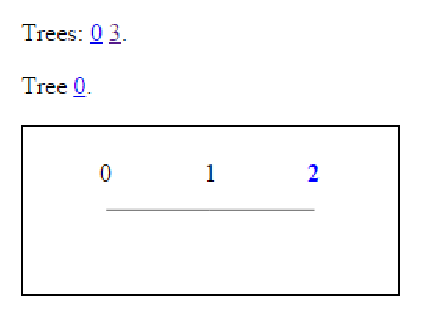
\includegraphics[scale=0.8]{ns_search_tree}
\caption[Needham-Schroeder search tree]{Search tree diagram for the
  initiator point of view in \texttt{ns.xhtml}}
\label{fig:ns init search tree}
\end{figure}

The search tree diagrams the steps in the search.  Each skeleton in
the entire graph file has a \index{label} label, a number starting
from 0.  The number associated with a tree is the label number of the
input skeleton.  The left edge of the search graph is the root of the tree:
in the case of Figure~\ref{fig:ns init search tree}, the graph does
not look very tree-like because the analysis doesn't branch.  The
numbers in the graph are the \index{label}labels of the skeletons
considered by {\cpsa} during its analysis, and clicking on a number
will direct the browser to display the corresponding skeleton.

The process by which {\cpsa} analyzes a skeleton is the repeated use
of an operation called the \index{cohort}\emph{cohort}, which takes an
input skeleton and produces a set of more refined skeletons that cover
all the possible executions the input skeleton covered.  The
relationship between a parent skeleton and a child is that a child is
included in the cohort calculated with the parent as an input.

\index{search tree}\index{search tree!colors} Numbers are normally
displayed in black, but may also be displayed in other colors.  Blue
numbers represent \emph{realized} skeletons, that is, skeletons that
may represent an actual execution.\footnote{Note that while realized
  skeletons already represent complete executions, \cpsa does further
  analysis once a realized skeleton is reached in order to
  \emph{generalize} that skeleton as much as possible.  A skeleton
  that is both realized and cannot be further generalized is a
  \index{shape}\emph{shape}.  See page \pageref{anchor:generalization}
  for more detail on generalization.}  Red numbers represent
\emph{dead} skeletons, that is, skeletons that represent partial
executions that are not part of any actual execution -- in other
words, impossible scenarios.

\index{skeleton!realized}\index{skeleton!dead} Numbers may occur in
the tree more than once, because it is possible that {\cpsa} will
discover a particular skeleton through more than one branch of the
analysis.  Green, italicized numbers represent skeletons present in
more than one branch that are not dead skeletons, while orange
italicized numbers represent dead skeletons present in more than one
branch.

Each skeleton starts with a line that indicates its label
(\texttt{item}) and the labels of its parent ((\texttt{parent}), if
any) and its children ((\texttt{child}), if any) See Fig.~\ref{fig:ns
  skel1}) The parent and child numbers link to those skeletons, while
the ``item'' number links back to the tree this skeleton is part of.

\begin{figure}
\centering
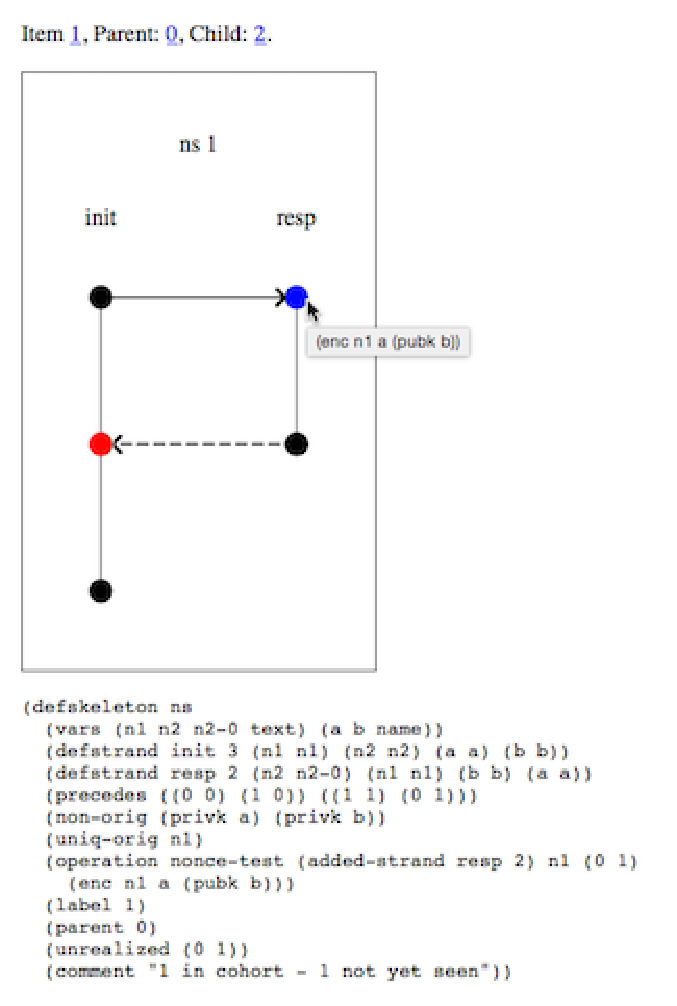
\includegraphics[height=7in]{ns_skel1_cursor}
\caption[Needham-Schroeder skeleton]{Skeleton from the initiator point
  of view in \texttt{ns.xhtml}}
\label{fig:ns skel1}
\end{figure}

Below the diagram is a \texttt{defskeleton} that fully describes the
skeleton.  This text is fully compatible with {\cpsa} input and can be
used as a skeleton input for analysis with this protocol, although
some of the fields in it are added by {\cpsa} and would be ignored
during input, for instance, the \texttt{label} and \texttt{parent}
fields.

The diagram shows the skeleton as a graph.  Strands are columns,
ordered from top to bottom.  The nodes in the graph are events,
normally transmissions or receptions of messages.  Nodes may be blue,
red, or black; a black node represents a transmission, while blue and
red nodes represent receptions.  A blue node represents an explainable
reception while a red node represents an unexplainable one.  The
left-most strands in a skeleton are normally the strands from the
input \texttt{defskeleton}.

\index{tooltip!skeleton node} The user may hover their mouse cursor
over any node and will see a display of the S-expression describing
the message at that event (see Figure~\ref{fig:ns skel1}). Here, if we
hover over the red node (as shown) we will see that this is an event where the
initiator receives the message $\enc{n1, n2}{K_a}$.  This occurs after
two transmissions: the first event in the init strand and the second
in the resp strand.  Those two transmissions are $\enc{n1, a}{K_b}$
and $\enc{n1, n2_0}{K_a}$.  Neither transmission is the expected
message, but sometimes a reception can be explained even if no regular
node sends the exact message.  Here, it is a question of what the
adversary can build given the messages available.  In this skeleton
there are \texttt{non-orig} or \texttt{uniq-orig} assumptions about
$n1, SK_a$, and $SK_b$, so since both messages are encrypted under
keys for which we have a secrecy assumption on the decryption key, the
adversary is unable to decrypt them.  The adversary is also unable to
build the required message: although the adversary is allowed access
to $n2$ and $K_a$ (since there are no restrictions on those), the
adversary does not have access to $n1$.  Hence, this node is
unexplainable.

Arrows in the diagram represent basic orderings in the skeleton;
arrows go from earlier events to later events.  An arrow is solid when
it goes from an event transmitting a message to one receiving the same
message. So the blue node in this example is obviously explained
because the exact message was transmitted by the initiator,
specifically, at the first node in the initiator strand.  The arrow
ending at the red node is dashed because the messages do not agree,
but it still represents that in this skeleton the second node of the
responder strand occurs before the second node of the initiator strand.

\section{Interpreting shapes}

Next, we turn our attention to Figure~\ref{fig:ns init shape}, which
is the one shape found by {\cpsa} during the search on the initiator
point of view.

\begin{figure}
\centering
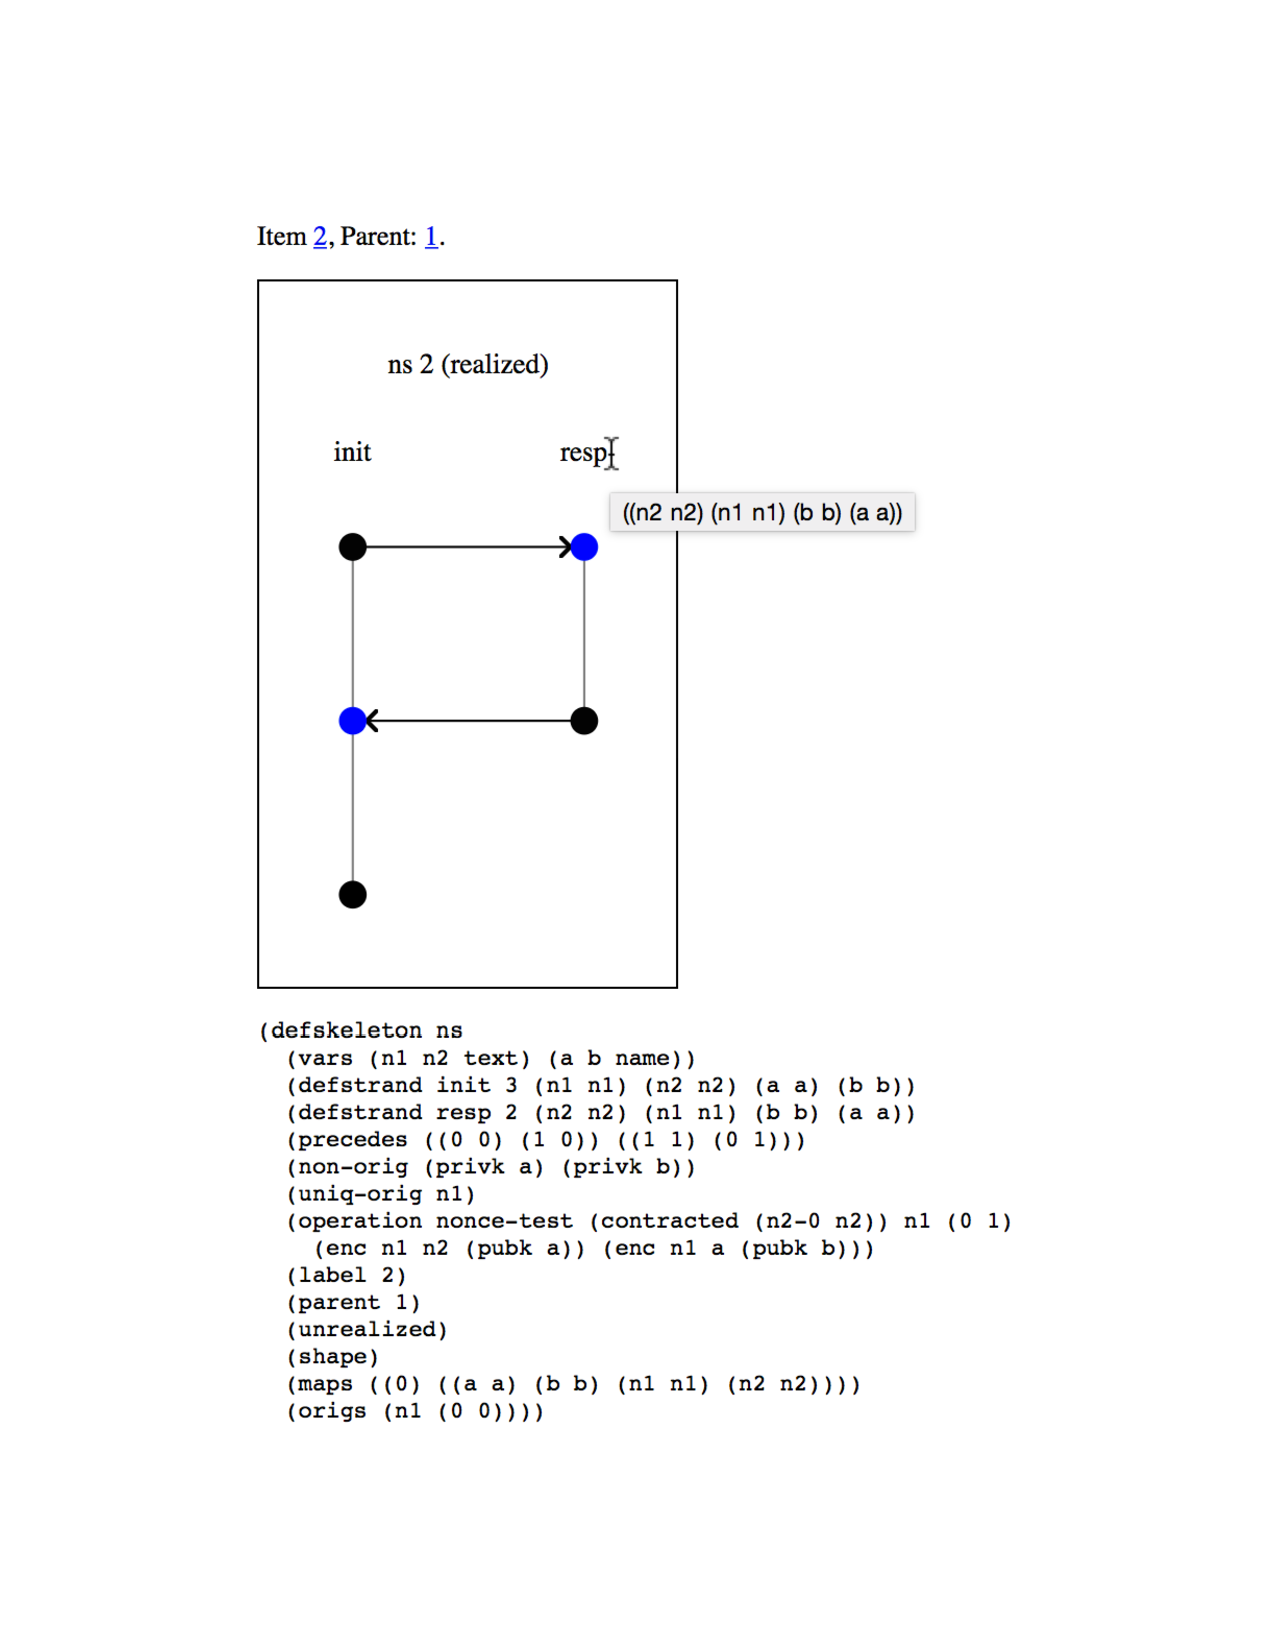
\includegraphics[height=7in]{ns_skel2_cursor}
\caption[NS shape, initiator point of view]{The only shape from the
  initiator point of view (\texttt{ns.xhtml})}
\label{fig:ns init shape}
\end{figure}

Before we get into detail on what is contained in this skeleton, note
the graph.  All the arrows are solid, and there are arrows everywhere
we expect them to be.  This describes a message being sent by an
initiator and received, unaltered, by a responder, who then sends a
message that is received, again unaltered, by the same initiator, who
then sends a message.

\index{tooltip!instance} The user can hover their mouse cursor over
the name of the role at the top of a strand in the skeleton diagram to
see the variable assignment used in that instance.  Here, hovering
over both the instances indicates that they are in agreement about the
values of $n1, n2, a$, and $b$: that is, the initiator's internal
value for each variable is the same as the responder's internal value
for the variable of the same name.

It may seem slightly odd that the initiator sends a message in its
third node that is not received by anyone, but we know that in general
it need not be received.  The adversary completely controls the network,
so it does not have to deliver that message.

\paragraph{The responder's point of view.}
The shape found during the search on the \emph{responder's} point of
view, however, includes something unusual.  See Figure~\ref{fig:ns
  resp shape}.

\begin{figure}
\centering
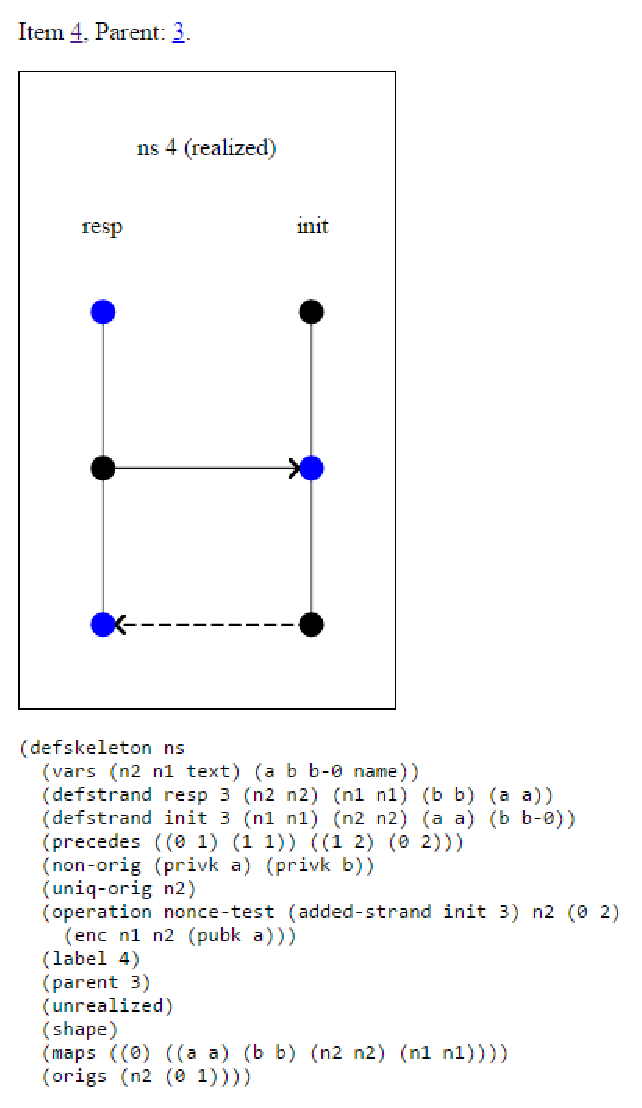
\includegraphics[scale=0.9]{ns_skel4}
\caption[NS shape for responder point of view]{The only shape in the
  responder point of view search in \texttt{ns.xhtml}}
\label{fig:ns resp shape}
\end{figure}

The graph of this shape should look less like expected behavior.  Two
things look odd, even at first glance.  Most noticeable is the dashed
arrow from the third initiator node to the third responder node.
Also, there's the fact that there is a blue node (the one in the top
left) that does not have any arrow coming in.

Inspection of the instances in this shape reveals that the initiator
and responder agree on all the values except for $b$.  This explains
the dashed arrow: the initiator sends $\enc{n2}{K_{b_0}}$ but the
responder receives $\enc{n2}{K_b}$; these messages are not the same,
which is why the arrow is not solid.  As for how the responder could
receive the proper value, note that we only assumed $SK_a$ and $SK_b$
are secure, but we did not assume $SK_{b_0}$ was secure.  It would have
been hard to do so, since $b0$ is a value we know nothing about from
the initiator's point of view. The initiator's transmission of
$\enc{n2}{K_{b_0}}$ thus does not protect $n2$ from decryption, so an
attacker could have created the responder's received message by
encrypting $n2$ under $K_b$.

The lack of an incoming arrow for the responder's first node can be
explained because of the lack of any assumption about the value $n1$.
The value $n1$ is the initiator's nonce, but this analysis does not
assume that an initiator, if present, will choose their nonce
properly.  So $n1$ could actually be a value already chosen by the
adversary, and the message $\enc{n1,a}{K_b}$ can be constructed and
delivered to the responder before the initiator even starts.

The fact that the initiator and responder do not agree on $b$ is an
interesting feature of this protocol.  We know from the initiator's
point of view that the initiator $a$, when they have completed their
execution, can infer that $b$ has taken part in the responder role
with $a$, and that they agree on both nonces.

The responder's point of view leads to less information.  The
responder $b$ knows that $a$ has taken part in the initiator role, but
does not know that $a$ intended to initate communication with $b$.
This lets us conclude that the Needham-Schroeder protocol provides
less than an ideal level of authentication.

\index{Lowe attack}
\index{Needham-Schroeder-Lowe protocol}
\begin{exercise}
  The attack described above was first identified by Gavin
  Lowe~\cite{Lowe96a}, who also proposed a fix, namely, to have the
  second message in the Needham-Schroeder protocol include the name
  $b$ of the responder.

Make a copy of the Needham-Schroeder input file and modify the
protocol so that the second message (in both roles) includes a $b$.
Run the analysis again and graph it.  You should observe that the
disagreement on $b$ from the responder's point of view is no longer
possible, and that the initiator's point of view is still good.
\end{exercise}

\section{Blanchet's simple example protocol}
\label{sec:blanchet}

\index{Blanchet protocol} \index{examples!Blanchet} Next we turn our
attention to a second protocol, which will help build the reader's
experience with {\cpsa} and also introduce some additional features.
This protocol is due to Bruno Blanchet, and has a flaw introduced by
design for the purpose of discussing protocol analysis.  In this
protocol there are again two participants: an initiator and a
responder.  However, in this protocol, we do not use names, just
public keys.  Specifically, one party has a public signing key ($a$),
while the other has a public encryption key ($b$).

The protocol is as follows, informally:

\begin{itemize}

\item The initiator chooses a fresh, random session key $s$, signs it
  with their private signing key (corresponding to the public key
  $a$), and encrypts it with the responder's public key $b$ and sends
  the result to the responder.

\item The responder receives and decrypts such a message, confirms the
  signature, and then encrypts a piece of data $d$ under $s$ and sends
  this back to the initiator.
\end{itemize}

The file \texttt{blanchet.scm} in the examples directory contains
Blanchet's simple example protocol described above.  See
Figure~\ref{fig:blanchet defprotocol} for the protocol declaration.

\begin{figure}
\centering
\begin{tabular}{l}
\verb|(defprotocol blanchet basic|\\
\verb|  (defrole init|\\
\verb|    (vars (a b akey) (s skey) (d data))|\\
\verb|    (trace (send (enc (enc s (invk a)) b))|\\
\verb|           (recv (enc d s)))|\\
\verb|    (uniq-orig s))|\\
\verb|  (defrole resp|\\
\verb|    (vars (a b akey) (s skey) (d data))|\\
\verb|    (trace (recv (enc (enc s (invk a)) b))|\\
\verb|           (send (enc d s)))|\\
\verb|    (uniq-orig d)))|
\end{tabular}
\caption{The Blanchet simple example protocol}
\label{fig:blanchet defprotocol}
\end{figure}

\ttindex{akey} \ttindex{skey} \ttindex{data} There are several
elements of this protocol input that are new.  First of all, the
Needham-Schroeder protocol used only two types: \texttt{name} and
\texttt{text}, while this protocol uses three new types.  The
\texttt{data} type is for simple values, much like \texttt{text}.  In
fact, the two types are interchangeable, but both are available for
cases where an analyst may wish to describe a protocol in which two
types of simple values exist that cannot be confused for each other.

The \texttt{akey} and \texttt{skey} types are for keys, specifically,
asymmetric and symmetric keys, respectively.  The \texttt{invk}
function symbol maps an asymmetric key to its inverse.

\index{signatures} Note that we use \texttt{(enc s (invk a))} to
represent the digital signature.  A digital signature in the {\cpsa}
message algebra is represented as an encryption under the signature
key.

\index{role declarations} A third feature is the presence of a
delcaration such as \texttt{(uniq-orig s)} within a
\texttt{defrole}.  Like the \texttt{uniq-orig} declaration that can
appear in a skeleton, this declaration indicates that the value
contained inside is freshly chosen.  When this declaration appears in
the role, however, the assumption is that the value is freshly chosen
by \emph{every} honest participant in the protocol who plays that
role.  Declarations present in a role are inherited by every skeleton
with an instance of that role.  See Chapter~\ref{ch:declarations} for
more on the declarations supported by \cpsa.

\begin{exercise}
Make a variant of the Needham-Schroeder protocol in which the
freshness of each party's nonce is assumed via a \texttt{uniq-orig}
declaration in the protocol role.  Run the analysis from each
participant's point of view.  What differs in the shapes, and why?
(There should be one difference that's noticeable in the graph of one
of the shapes.)
\end{exercise}

\begin{exercise}
Make a variant of the Needham-Schroeder protocol in which the secrecy
of each party's partner's private key is assumed via a
\texttt{non-orig} declaration in the protocol role.  Run the analysis
from each participant's point of view.

You should observe that the authentication failure is no longer
present in the shape from the analysis of the responder's viewpoint.
What conclusion can you draw about this declaration?  Did we fix the
protocol?  If not, why does the analysis seem to contain no flaws?
\end{exercise}

The \texttt{blanchet.scm} file contains four inputs to the analysis.
The first and second are just the points of view of each participant,
under typical assumptions.  But the third and fourth contain another
new element.  See Figure~\ref{fig:blanchet pov3-4} for these two
inputs.

\begin{figure}
\centering
\begin{tabular}{l}
\verb|(defskeleton blanchet|\\
\verb|  (vars (a b akey) (s skey) (d data))|\\
\verb|  (defstrand init 2 (a a) (b b) (s s) (d d))|\\
\verb|  (deflistener d)|\\
\verb|  (non-orig (invk b)))|\\\\
\verb|(defskeleton blanchet|\\
\verb|  (vars (a b akey) (s skey) (d data))|\\
\verb|  (defstrand resp 2 (a a) (b b) (s s) (d d))|\\
\verb|  (deflistener d)|\\
\verb|  (non-orig (invk a) (invk b)))|\\\\
\end{tabular}
\caption{Blanchet points of view}
\label{fig:blanchet pov3-4}
\end{figure}

\ttindex{deflistener}\index{listener} These two inputs are prepared to
ask a confidentiality question: specifically, is the value $d$ exposed
to the adversary?  A \emph{listener} is a pseudo-role that is
considered part of all protocols by {\cpsa}.  That role consists of
receiving some arbitrary message and then sending that same message.
Listeners can show up in {\cpsa} analyses, in order to handle a case
where a certain value is learnable, so that the rest of the case
breakdown can assume that value is not learnable.

\index{skeleton!dead}
In this protocol, the secret data $d$ remains private in the
initiator's point of view.  Figure~\ref{fig:blanchet tree 6} shows the
search tree for the point of view in which the initiator completes the
protocol and in which there is a listener for the same $d$ value the
initiator hears.  The fact that all the numbers are red here indicates
that all the skeletons in the search are ``dead'', meaning that they are
inconsistent with any actual executions.  In other words, there are no
executions in which $d$ is revealed given our assumption that the private
decryption key of $b$ is not compromised.

However, $d$ does not remain private in the responder's point of view.
Figure~\ref{fig:blanchet skel 13} shows the graph of a shape for the
point of view in which the responder completes the protocol and in
which there is a listener for the $d$ value the responder sends.  Note
that although $d$ is encrypted under $s$, and $s$ is freshly chosen by
an initiator, the shape shows that $s$ can leak.  We are not
guaranteed that the initiator and responder agree on $b$.  Therefore,
the initiator may have sent $s$ encrypted with $b_0$, and since the
private key corresponding to $b_0$ is not necessarily secret, $s$ may
leak.

\begin{figure}
\centering
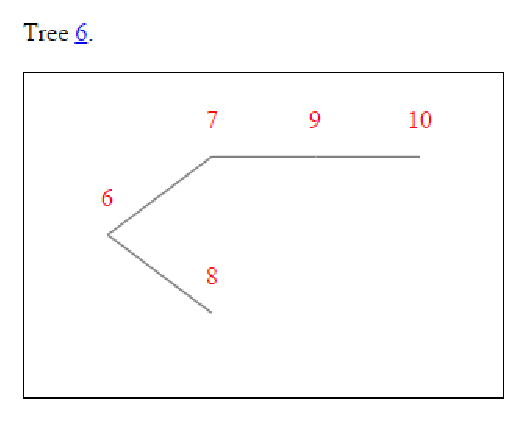
\includegraphics{blanchet_tree6}
\caption[Blanchet privacy search tree]{The search tree for the privacy
  of $d$ in the initiator's point of view in \texttt{blanchet.xhtml}}
\label{fig:blanchet tree 6}
\end{figure}

\begin{figure}
\centering
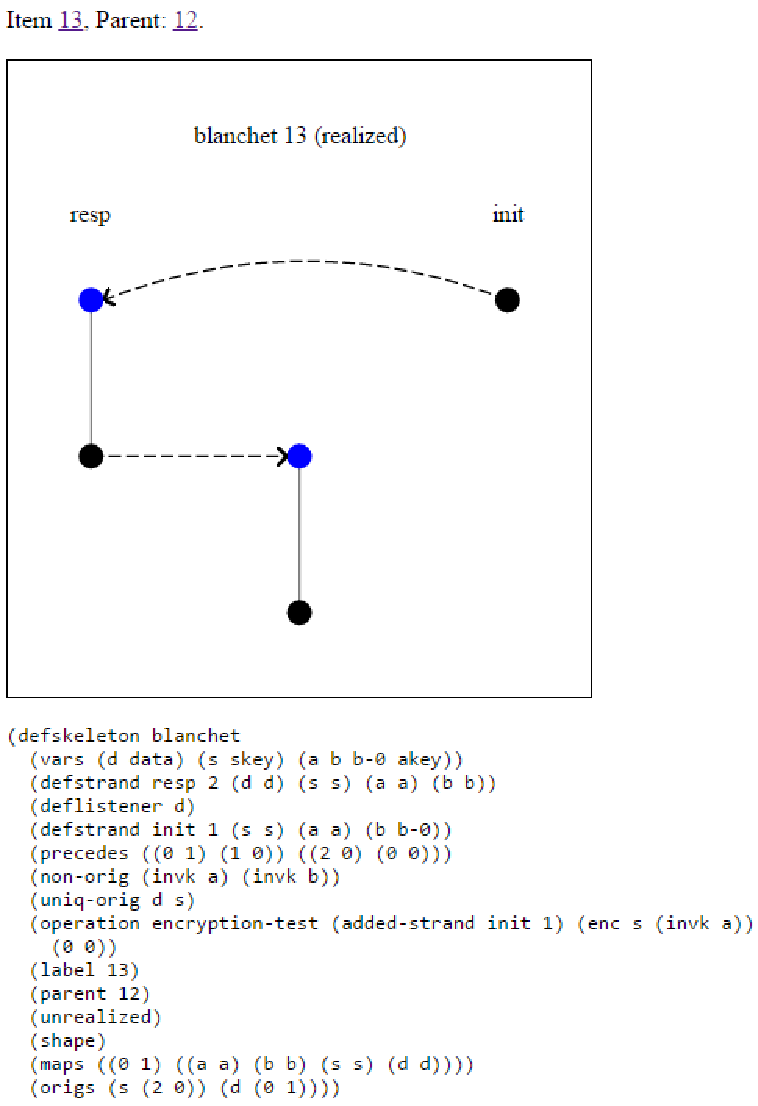
\includegraphics[scale=0.9]{blanchet_skel13}
\caption[Blanchet shape for responder's point of view]{The only shape
  in the analysis for the responder's point of view with a listener
  for $d$ in \texttt{blanchet.xhtml}.  The second strand, with no role
  name, is the listener. }
\label{fig:blanchet skel 13}
\end{figure}

The \texttt{blanchet.scm} file also contains a second protocol with
the name \texttt{blanchet-corrected} in which the flaw that allows $d$
to be learned in the responder's point of view is eliminated.

\begin{exercise}
  Modify the Blanchet protocol to add a role that is identical to the
  initiator role, except that $s$ is not declared \texttt{uniq-orig}.
  What impact does this have on the analyses?
\end{exercise}

\begin{exercise}
  If you modify the Blanchet protocol to instead add a role that is
  identical to the responder role, except that $d$ is not declared
  \texttt{uniq-orig}, what impact do you believe this will have on the
  analyses?  Make a prediction, then check your prediction.
\end{exercise}

\begin{exercise}
\label{ex:noroledecls_blanchet}
Try modifying the Blanchet protocol, removing the \texttt{uniq-orig}
declarations from the two roles.  Replace the \texttt{defskeleton}s in
the input file with the point of view skeletons for the un-corrected
version of the Blanchet protocol from \texttt{blanchet.xhtml}; these
skeletons will explicitly include declarations that would be inherited
but were lost due to the removal of the role declaration.
\end{exercise}

\begin{exercise}
Starting from your modified version of the Blanchet protocol from
Exercise~\ref{ex:noroledecls_blanchet}, add a \texttt{uniq-orig} declaration
on $s$ to the point of view with a responder instance and a listener for $d$.

This should produce an error message, because {\cpsa} expects that for
every value declared to be uniquely originating, that value originates
at some point in the skeleton.  When only the responder's strand and
the listener are present, $s$ does not originate; it is received by
the responder before being used in an outgoing message, and it does
not occur on the listener strand at all.

Now add a \texttt{defstrand} adding an instance of an initiator
(height 1), using the same $s$, and declare $s$ to be uniquely
originating.  Check that the resulting shape is the same attack shape
as in the unmodified \texttt{blanchet.xhtml}.
\end{exercise}

%  See Section~\ref{sec:role_decls2} for more about how role
%  declarations work. 

%%% Local Variables:
%%% mode: latex
%%% TeX-master: "cpsa4manual"
%%% End:

\chapter{Algebra Features of CPSA}
\label{ch:algebra}

\index{Diffie-Hellman!algebra}
The {\cpsa} distribution comes equipped with two cryptographic
alegbras, the \texttt{basic} cryptoalgebra and the
\texttt{diffie-hellman} cryptoalgebra.  The Diffie-Hellman algebra is
a pure extension of the basic algebra, so a user may always use the
Diffie-Hellman algebra to access all algebraic features.  However, the
performance of the tool is superior when using the basic algebra, so
users are advised to choose the basic algebra whenever they are not
making use of Diffie-Hellman features.

In Chapter~\ref{ch:basic}, we introduced the basic cryptoalgebra,
along with the \texttt{data, text, name, skey,} and \texttt{akey}
sorts, and the \texttt{pubk, privk, invk, enc,} and \texttt{cat}
function symbols.  In addition to these, the basic cryptoalgebra
contains the sorts \ttindex{tag} \texttt{tag} and \texttt{mesg}, and the \texttt{ltk}
and \texttt{hash} function symbols, and string constants.

The Diffie-Hellman cryptoalgebra introduces three further sorts,
\texttt{base, rndx,} and \texttt{expt}, and six new function symbols,
\texttt{bltk, exp, rec, mul, gen,} and \texttt{one}.  For performance
reasons, one should always avoid using variables of sort
\texttt{base}.  Instead, replace the variable with \texttt{(exp (gen)
  x)}, where \texttt{x} is a variable of sort \texttt{expt}.

In this chapter we will explain these additional features with
examples.  In Section~\ref{sec:kerberos}, we will discuss the
\texttt{ltk} function symbol and the use of the \texttt{mesg} sort,
worked with an example based on the Kerberos protocol.  In
Section~\ref{sec:dh}, we will discuss the tool's Diffie-Hellman
features.  In Section~\ref{sec:other_algebra}, we will discuss the
remaining features, and note examples that demonstrate their use.
For a more complete reference about the two algebras, see Section~\ref{sec:algebra_ref}.

\section{Generic messages and long-term keys}
\label{sec:kerberos}

\index{Kerberos protocol}
\index{examples!Kerberos}
Securing communications purely with symmetric keys faces an inherent
scaling problem: when there are $n$ parties that may wish to
communicate, there must be $O(n^2)$ keys shared between parties, which
gets to be too many in any system with a large number of users.

The Kerberos protocol is a well-known protocol for the distribution of
symmetric keys.  Instead of having the $n$ parties share keys with
each other party, the users share a key only with a central key server
(also known as a key distribution center).  The key server controls
key distribution within a \emph{realm} that can be thought of as the
set of users that share keys with the key server.

Suppose a user wishes to communicate securely with another user in the
same realm.  The first user would contact the key server and request a
session key for communication with the other user.  The key server
could then encrypt the session key twice, once under each user's
shared key with the server.  One encrypted key is sent back to the
user that requested the channel, and the other (called the ``ticket'')
is also sent to the requesting user, to be forwarded on to their
communication partner.

We will focus on a flawed protocol similar to the initialization
protocol used by Kerberos.  The protocol is described informally as
follows.  There are three parties, the initiator $a$, the responder
$b$, and the key server $s$.

\begin{itemize}

\item $a$ sends a message $(a, b, n)$ to the key server, where $n$ is
  a freshly chosen nonce.

\item The key server, on a message $(a, b, n)$, picks a fresh, random
  session key $k$, and sends two encryptions to $a$:
  $\enc{k,n}{SK(a,s)}$ and $\enc{k,a,b}{SK(b,s)}$.  Here, $SK(x,s)$
  refers to the shared secret between the key server and~$x$.

\item $a$ receives these two messages, decrypts the first to learn $k$
  and to check that the proper nonce $n$ was included, then sends a
  message $m$ on to the responder, encrypted under $k$, along with the
  second message (the ticket).

\item $b$ receives two encrypted messages, decrypts the second to
  learn $k$, and decrypts the first with $k$ to learn the message.
\end{itemize}

\ttindex{ltk} The \texttt{ltk} function symbol is used in {\cpsa} to
represent long-term shared keys between two specific parties, when
communication of that key is assumed out of scope of the analysis.
See Figure~\ref{fig:kerb-flawed defprotocol} for a
\texttt{defprotocol} that attempts to describe this flawed version of
the Kerberos initialization protocol.  See \texttt{kerb.scm} in the
examples directory for the input file discussed here.

\begin{figure}
\centering
\begin{tabular}{l}
\verb|(defprotocol kerb-flawed basic|\\
\verb|  (defrole init|\\
\verb|    (vars (a b s name) (m n text) (k skey))|\\
\verb|    (trace (send (cat a b n))|\\
\verb|           (recv (cat (enc k n (ltk a s)) (enc k a b (ltk b s))))|\\
\verb|           (send (cat (enc m k) (enc k a b (ltk b s)))))|\\
\verb|    (uniq-orig n))|\\
\verb|  (defrole keyserv|\\
\verb|    (vars (a b s name) (n text) (k skey))|\\
\verb|    (trace (recv (cat a b n))|\\
\verb|           (send (cat (enc k n (ltk a s)) (enc k a b (ltk b s)))))|\\
\verb|    (uniq-orig k))|\\
\verb|  (defrole resp|\\
\verb|    (vars (a b s name) (m n text) (k skey))|\\
\verb|    (trace (recv (cat (enc m k) (enc k a b (ltk b s)))))))|\\
\end{tabular}
\caption{A flawed version of Kerberos}
\label{fig:kerb-flawed defprotocol}
\end{figure}

The actual Kerberos protocol contains several additional elements that
we omit for simplicity, but the key difference is that the message
encrypted under $SK(a,s)$ should include $b$.  The message from the
initiator that requests a session key is transmitted in the clear and
can be tampered with, so the initiator needs assurance that the
session key $k$ is being exposed only to the initiator and $b$.
Otherwise, even assuming the long-term keys of both $a$ and $b$ with
the key server are secure, a third party may observe the message $m$:
all the adversary has to do is block the initial message and substitute
$b$ with another name $c$.

Will {\cpsa} find this attack?  See \texttt{kerb.xhtml} for the
results of the analysis for the point-of-view skeleton described in
Figure~\ref{fig:kerb-flawed-pov}.  Note the use of
\texttt{defstrandmax}; this is a shortcut you can use in \cpsa to
specify a full-height instance of a role.

\begin{figure}
\centering
\begin{tabular}{l}
\verb|(defskeleton kerb-flawed|\\
\verb|  (vars (a b s name) (m text))|\\
\verb|  (defstrandmax init (a a) (b b) (s s) (m m))|\\
\verb|  (deflistener m)|\\
\verb|  (non-orig (ltk a s) (ltk b s))|\\
\verb|  (uniq-orig m))|\\
\end{tabular}
\caption{Flawed Kerberos point of view}
\label{fig:kerb-flawed-pov}
\end{figure}

Interestingly, the result of the analysis does not indicate any attack
is possible!  The analysis gets stuck at a skeleton (see
Figure~\ref{fig:kerb-skel4}) where the key server does in fact
generate a session key for $a$ and $b$, and where that session key is
exposed, but it cannot be exposed if it was generated for $a$ and $b$
and if we are assuming both of their long-term keys are private.

\begin{figure}
\centering
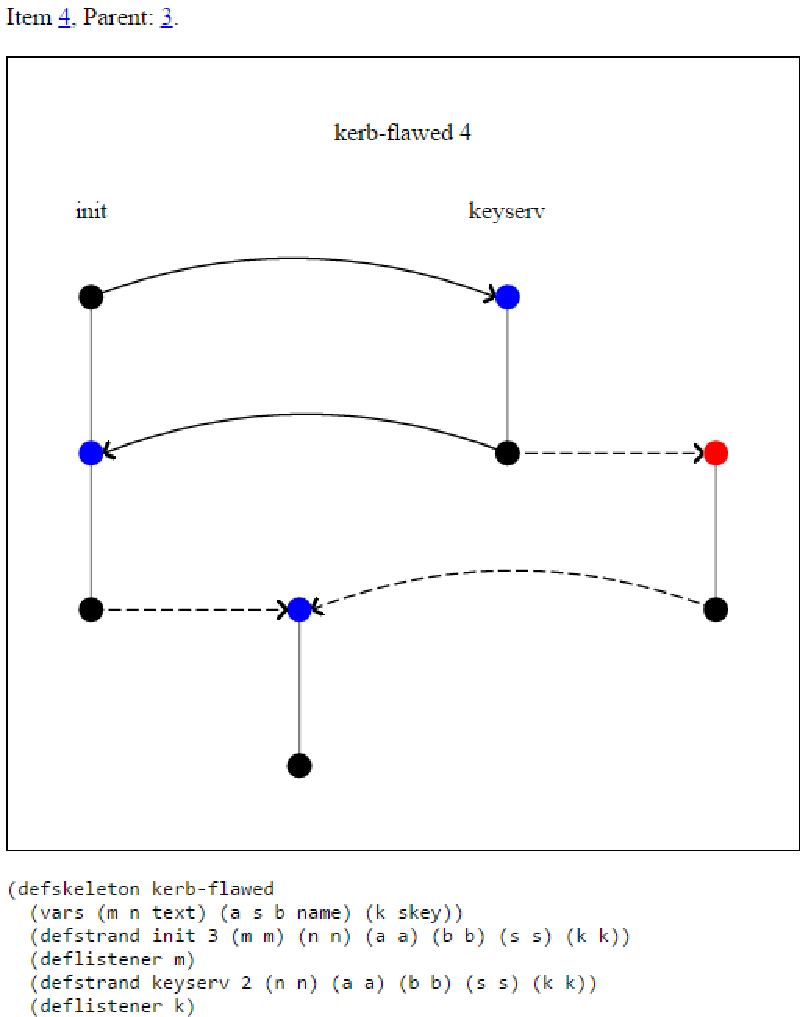
\includegraphics{kerb_skel4}
\caption[Flawed Kerberos dead skeleton]{Flawed Kerberos dead skeleton.  The use of the \texttt{mesg} sort provides a fix to this badly modeled version of the protocol.}
\label{fig:kerb-skel4}
\end{figure}

\ttindex{mesg} \index{generics} The reason {\cpsa} gets the wrong
result here is that we have inadvertently modeled our protocol
question incorrectly.  Specifically, we have described a version of
the protocol where the initiator is able to check the validity of the
ticket.  The attack we have in mind is one where the two encrypted
keys received by the initiator are prepared by a key server instance,
but one which does not agree with the initiator on $b$.  However, the
ticket would not match what the initiator expects in our expression of
the initiator role.\footnote{An alert reader may wonder how they could
  detect such an error of their own when using the tool.  We will
  return to this example in Chapter~\ref{ch:algorithm}, when we
  discuss how the {\cpsa} search process works.}

We described an initiator that will only proceed onto the third step
(sending $m$) if the ticket is of the form we specified.  In fact, the
initiator cannot do this.  The initiator cannot even verify that the
ticket is encrypted under the correct key! The solution is to use a
generic variable, one that can stand for any message, even one that a
particular participant cannot parse or understand.  The \texttt{mesg}
sort is the sort of all possible messages, so a variable of the
\texttt{mesg} sort can stand for any potential value at all.  See
Figure~\ref{fig:kerb-flawed2 defprotocol} for a version that models
the initiator's reception properly.  Note the \texttt{ticket} variable
in the initiator role, which stands for the ticket value the initiator
cannot inspect.

\begin{figure}
\begin{center}
\begin{tabular}{l}
\verb|(defprotocol kerb-flawed2 basic|\\
\verb|  (defrole init|\\
\verb|    (vars (a b s name) (m n text) (ticket mesg) (k skey))|\\
\verb|    (trace (send (cat a b n))|\\
\verb|           (recv (cat (enc k n (ltk a s)) ticket))|\\
\verb|           (send (cat (enc m k) ticket)))|\\
\verb|    (uniq-orig n))|\\
\verb|  (defrole keyserv|\\
\verb|    (vars (a b s name) (n text) (k skey))|\\
\verb|    (trace (recv (cat a b n))|\\
\verb|           (send (cat (enc k n (ltk a s)) (enc k a b (ltk b s)))))|\\
\verb|    (uniq-orig k))|\\
\verb|  (defrole resp|\\
\verb|    (vars (a b s name) (m n text) (k skey))|\\
\verb|    (trace (recv (cat (enc m k) (enc k a b (ltk b s)))))))|\\
\end{tabular}
\end{center}
\caption[Flawed Kerberos with a generic ticket]{Using a variable of
  sort \texttt{mesg} in a flawed version of Kerberos}
\label{fig:kerb-flawed2 defprotocol}
\end{figure}

This version of the flawed Kerberos protocol may also be found in the
file \texttt{kerb.scm}, and its analysis may be found in
\texttt{kerb.xhtml}.  This time, there is a shape found.  See
Figure~\ref{fig:kerb-skel7}.

\begin{figure}
\centering
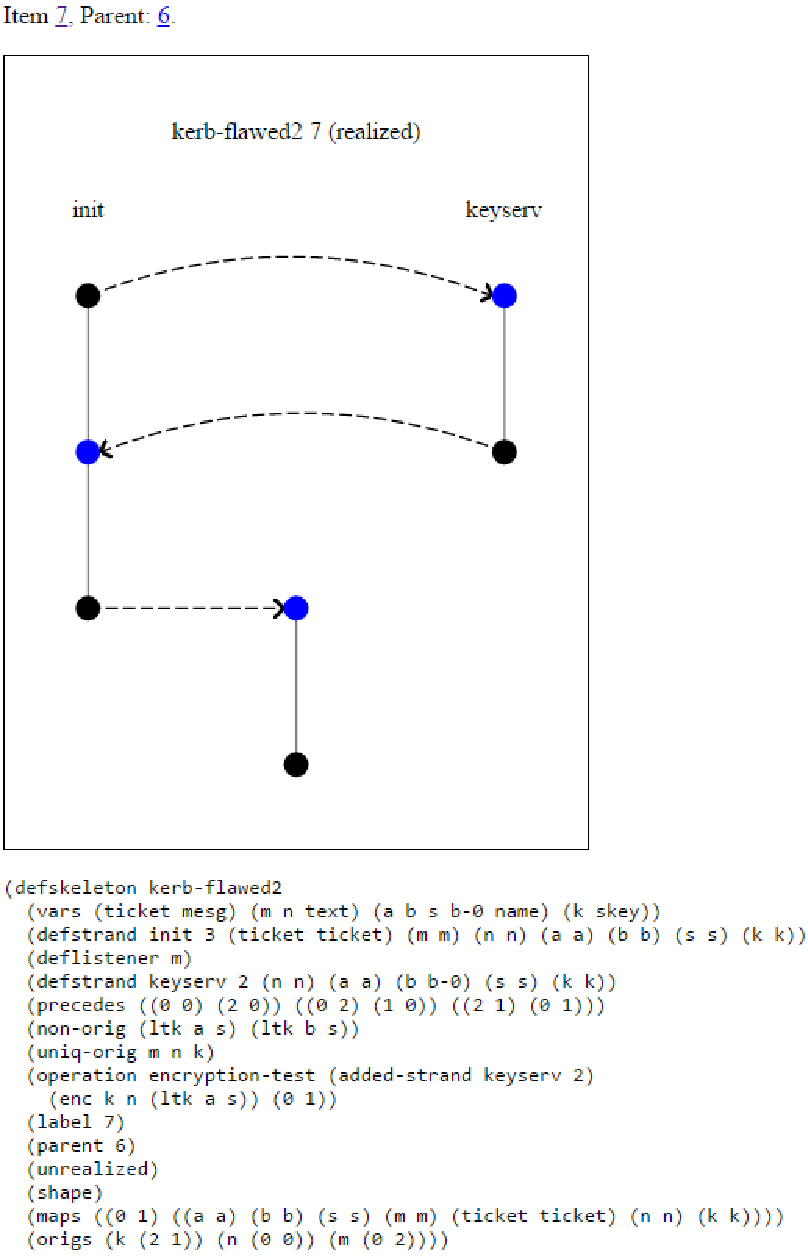
\includegraphics[scale=0.8]{kerb_skel7}
\caption[Flawed Kerberos shape]{Flawed Kerberos shape.  The use of the \texttt{mesg} variable allows us to find the attack illustrated here.}
\label{fig:kerb-skel7}
\end{figure}

\paragraph{Notes on generic variables.}
Variables of the \texttt{mesg} sort are constrained in {\cpsa}, and
may only be used when they are received before they are transmitted.
So for instance the $m$ variable in the initiator role of the flawed
Kerberos protocol cannot be of the \texttt{mesg} sort, because it
appears first in a transmission. However, if the responder is willing
to accept an encryption of any message $m$, then $m$ may declared as a
variable of the \texttt{mesg} sort within that role.

Also, variables of the \texttt{mesg} sort should never be used as a
key in any encryption.  This is because {\cpsa} uses a single function
symbol to represent both symmetric and asymmetric encryption, and when
the key is a variable of sort \texttt{mesg}, it is ambiguous which is
meant.

\paragraph{Notes on long-term keys.}
\ttindex{ltk}
Long-term keys are uni-directional: \texttt{(ltk a b)} and
\texttt{(ltk b a)} are distinct values.  In fact, {\cpsa} believes
that they cannot be the same unless $a = b$.  This is fine for
modeling protocols like Kerberos where there is a clear distinction
between client and server behavior.  Note that in our protocol
example, all long-term keys were described in all roles with a client
name in the first position and a server name in the second position.
See Section~\ref{sec:bltk} for discussion of the
\texttt{bltk} function symbol, which models \emph{bi-directional}
long-term symmetric keys.

\index{Yahalom protocol}\index{examples!Yahalom}
For another example of the use of long-term symmetric keys in a
protocol, see \texttt{yahalom.scm} in the examples directory.

\begin{exercise}
\label{ex:fix_kerberos}
Fix the flawed version of Kerberos so that the initiator can believe
their transmission is private to them and $b$.  Continue to use the
ticket variable of sort \texttt{mesg}.

Construct a \texttt{defskeleton} for the responder's point of view
for your fixed protocol, analyze it, and explain in English what
authentication property this analysis implies.
\end{exercise}

\begin{exercise}
  Construct a \texttt{defskeleton} for the initiator's point of view,
  without the listener for $m$, in the fixed version you created in
  Exercise~\ref{ex:fix_kerberos}.  Run the tool on your
  \texttt{defskeleton}.  Why are there dashed arrows in the result?
  Does this represent an insecurity in the protocol?

Whether or not you think this is an insecurity, think about how you
would alter the protocol to avoid the dashed arrows, and try out your
ideas.
\end{exercise}

\index{Otway-Rees protocol} \index{examples!Otway-Rees} The Otway-Rees
protocol is another example of very similar modeling; see
\texttt{or.scm} and \texttt{or.xhtml} if you wish to explore these
issues further on your own.

\section{Modeling Diffie-Hellman}
\label{sec:dh}

\index{Diffie-Hellman}
In their seminal 1976 paper, ``New Directions in Cryptography'',
Diffie and Hellman proposed the notion of public-key cryptography
\cite{DiffieHellman76}.  They did not have a method for public-key direct
encryption, but they did have a key exchange protocol that has become
a crucial building block in cryptographic protocols.

The Diffie-Hellman protocol works as follows.  A large prime number
$p$ is chosen and agreed upon as a parameter, and $g$ is chosen to be
some integer modulo $p$.  In order to enable secure communication
between arbitrary parties, Diffie and Hellman imagined a directory of
public values, like a phone book.  Each person who wishes to be able
to communicate securely with others will generate for themselves a
private value $x$, and publicize $g^x \bmod p$ as their public value.
If Alice's private value is $a$, and Bob's private value is $b$, then
the shared secret between Alice and Bob would be $g^{ab} \bmod p$,
which each party can calcuate from their own private value and their
partner's public value.  For instance, Alice can calculate $g^{ab}
\equiv (g^b)^a \bmod p$.

Version 3 of {\cpsa} introduces the Diffie-Hellman algebra, which
allows for analysis of protocols that incorporate Diffie-Hellman
techniques.  The Diffie-Hellman algebra includes all the function
symbols and sorts available in the basic algebra, plus three
additional sorts: two sorts (\texttt{rndx} and \texttt{expt}) for
exponents such as $x$, and \texttt{base}, for exponentiated values
such as $g^x$.  The Diffie-Hellman specific functions symbols are as
follows:

\begin{itemize}
\item \texttt{exp} represents exponentation.  For example, $h^x$ is
encoded as \\ \texttt{(exp h x)}.
\item \texttt{mul} represents multiplication of exponents.  So if $x$
is an exponent, \\ \texttt{(mul x x)} would represent the square of $x$.
\item \texttt{gen} represents the standard generator $g$.  It is
  probably best to think of \texttt{gen} as a constant, i.e. a
  function symbol with arity~0.

\item \texttt{one} represents the multiplicative identity for the group of
exponents.  Like \texttt{gen}, \texttt{one} is a 0-ary function.

{\bf Important: } \texttt{gen} and \texttt{one} are functions, so they
must be enclosed in parentheses.  So \texttt{(exp (gen) x)} represents
$g^x$, while \texttt{(exp gen x)} would represent ${gen}^x$ where
${gen}$ is expected to be a variable.  Similarly, \texttt{(mul (one)
  x)} represents $1 \cdot x$ while \texttt{(mul one x)} would
represent $one \cdot x$ where the tool expects $one$ to be an exponent
variable.

\item \texttt{rec} represents the multiplicative inverse in the group
  of exponents.  So for instance \texttt{(exp (exp (gen) x) (rec x)) =
    (exp (gen) (one)) = (gen)}.
\end{itemize}

At this time, {\cpsa} does not model addition of exponents, although
there are many examples of protocols that add or subtract exponents.
There is no way to take a product of exponentiated values either
(e.g. $g^x \cdot g^y$) since this would be equivalent to including
addition of exponents.

\index{Diffie-Hellman!unauthenticated}
\index{Diffie-Hellman!plain}
\index{examples!Diffie-Hellman}
Several examples of Diffie-Hellman protocols are available in the examples
directory of the distribution.  The \texttt{plaindh.scm} example models
a simple, unauthenticated Diffie-Hellman exchange between two parties.

The initiator and responder perform a Diffie-Hellman exchange, followed by
the initiator choosing a random nonce $n$ and sending it, encrypted with the
Diffie-Hellman key, to the responder, who decrypts $n$ and sends it back.

The analysis result can be found in \texttt{plaindh.xhtml}.  You can see
there that a shape is found where an initiator exists but no
responder; the $n$ can be decrypted because $g^{x x_0}$ can be
calculated by the adversary when $x_0$ is not assumed secret.

Two features of the {\cpsa} model of Diffie-Hellman in this protocol are
worth drawing attention to.  See Figure~\ref{fig:plaindh defprotocol}

\begin{figure}
\begin{center}
\begin{tabular}{l}
\verb|(defprotocol plaindh diffie-hellman|\\
\verb|  (defrole init|\\
\verb|    (vars (x rndx) (y expt) (n text))|\\
\verb|    (trace (send (exp (gen) x))|\\
\verb|           (recv (exp (gen) y)) |\\
\verb|           (send (enc n (exp (gen) (mul y x))))|\\
\verb|           (recv n))|\\
\verb|    (uniq-orig n)|\\
\verb|    (uniq-gen x))|\\
\verb| ...)|
\end{tabular}
\end{center}
\caption{Diffie-Hellman defprotocol}
\label{fig:plaindh defprotocol}
\end{figure}

\ttindex{rndx} \ttindex{expt}
Note that the initiator uses a variable $x$ of the \texttt{rndx} sort
to represent its own random variable, and a variable $y$ of the
\texttt{expt} sort to represent the exponent present in the base value
it receives from the initiator.  Distinct values of the \texttt{rndx}
sort model distinct independent random choices of exponents, while
\texttt{expt} values merely represent arbitrary exponents which may or
may not be calculated as some product of other known values.  Here,
since the initiator chooses their own exponent, we model $x$ as an
\texttt{rndx} value.  But since the initiator cannot know how the base value
$g^y$ was calculated, we model $y$ as an \texttt{expt} value.

Note that unlike the example in Section~\ref{sec:kerberos},
where receiving a specifically formatted encryption in a protocol role
implied the ability to decrypt and check that structure is present,
the use of a value like $g^y$ in a reception does not imply that $y$
is \emph{known}, only that $y$ is defined to be the value such that
$g^y$ is the base value received.

\ttindex{uniq-gen} Second, you may notice that $n$ is declared
\texttt{uniq-orig} while $x$ is declared \texttt{uniq-gen}.  The
difference between these declarations is rather technical: see
Section~\ref{sec:secrecy_assumptions} for details.  For the moment, it
is sufficient to say that one should use \texttt{uniq-gen} for
exponents that first occur within an exponentiation, rather than
\texttt{uniq-orig}.

\label{anchor:generalization}
\index{deletion} \index{generalization} It is also instructive to
examine the two final skeletons in the analysis that leads to the
shape; see Figure~\ref{fig:plaindh_skel4_5}.  The first realized
skeleton reached in the branch is skeleton 4, on the left, which
includes an instance of the initiator role and a listener.  But this
realized skeleton has a child: skeleton 5.  The difference is that
skeleton 5 does not include the listener.  This is an example of a
step that {\cpsa} takes called \emph{generalization}: when {\cpsa}
recognizes a realized skeleton (that is, one that has no unexplainable
receptions), it attempts to identify ways to make that skeleton more
general without losing coverage.  Here, {\cpsa} has deleted the
listener, because that actual explicit reception and re-transmission
of $g^{x x_0}$ is not strictly necessary.  When a realized skeleton
cannot be further generalized, {\cpsa} declares it a ``shape'' and
stops working in that branch of the analysis.

\begin{figure}
\centering
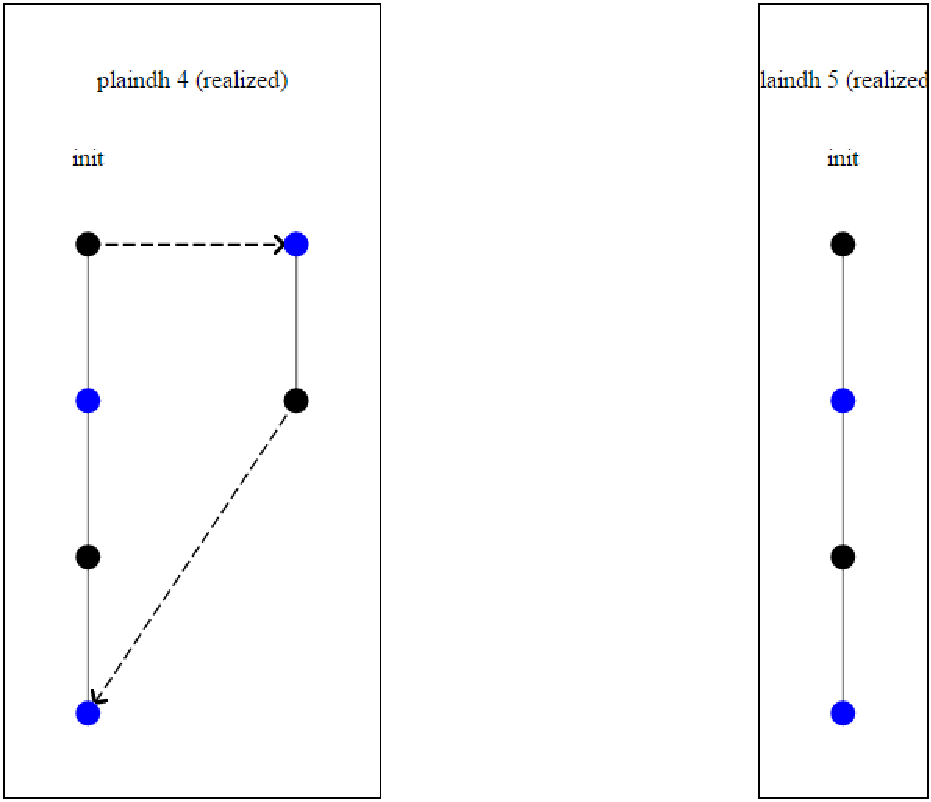
\includegraphics[scale=0.8]{plaindh_skel4_5}
\caption{Deletion of strand}
\label{fig:plaindh_skel4_5}
\end{figure}

\index{minimality of {\cpsa} output} You may notice there is another
shape in \texttt{plaindh.xhtml}, in which a responder is present.  As it
happens, the other shape is strictly less general than the shape shown
as skeleton 5.  {\cpsa} does not promise that the set of shapes it
outputs is strictly minimal, and this is one example where the output
of {\cpsa} is not minimal.

\subsection{Other examples}

\index{Station to Station protocol} \index{examples!Station to
  Station} The examples directory also contains the
\texttt{station.scm} and \texttt{station.xhtml} examples that model
the station-to-station protocol.  This protocol uses digital
signatures in order to authenticate a Diffie-Hellman exchange so that
the key established represents a secure and authenticated channel.
Two versions of the protocol are provided; in one, the Diffie-Hellman
exponents are assumed fresh in the roles, while in the other, they are
not.  The two analyses produce different results.

\index{forward secrecy}
\index{Unified Method} \index{examples!Unified Method} Another example
provided can be found in \texttt{iadh-um.scm} and
\texttt{iadh-um.xhtml}.  These inputs concern a method of determining
Diffie-Hellman session keys using both long-term and ``ephemeral''
exponents called the \emph{unified method}.  The ``ia'' in the example
name stands for \emph{implicitly authenticated}, because this method
of session key creation allows the parties to be sure that no other
party knows the key.  One interesting feature of this input is that it
contains an example of an exponent being transmitted outside of an
exponentiation.  Specifically, there is a role in which a party
generates and signs their long-term Diffie-Hellman public value, and
then compromises it by releasing the key.  The explicit compromise
allows us to test the ``forward secrecy'' property of the unified
method.

\section{Other Algebra Features}
\label{sec:other_algebra}

\subsection{Hashing}
\index{hash functions} \ttindex{hash} The {\cpsa} basic cryptoalgebra
includes a \texttt{hash} function symbol that can be used to represent
the use of a hash function.  The function takes a single input, but
\texttt{(hash t1 t2 ... tn)} is interpreted as shorthand for
\texttt{(hash (cat t1 (cat t2 ( \ldots tn) \ldots )))}.

\begin{exercise}
  The Needham-Schroeder protocol discussed in Chapter~\ref{ch:basic}
  was described as for key agreement, but no session key is apparent
  in the protocol.  The intention is to use the hash of the two nonces
  as the key.  Make a copy of the \texttt{ns.scm} example in which
  this key is explicitly used to encrypt and transmit a separate fresh
  value, and make a point of view testing the confidentiality of the
  plaintext.
\end{exercise}

\subsection{Constants}
\index{constants} \index{tags} \ttindex{tag} Numerous cryptographic
protocols make use of magic numbers or string constants to
disambiguate the purpose of various messages that occur during the
protocol.  {\cpsa} includes constant strings in the basic
cryptoalgebra.  Such constants always appear as quoted strings,
e.g. \texttt{"foo"}.  These strings do not need to be declared in a
\texttt{vars} statement because they are not variables.  Tags are
messages, so that a variable of
\verb|mesg| sort may be instantiated by a tag.

%   The sort of
%   string constants is always \texttt{tag}, which is a basic sort much
%   like \texttt{text} or \texttt{data}, however, it is strongly
%   recommended that the \texttt{tag} sort be used only for variables that
%   are intended to represent as-yet undetermined string constants.  See
%   Section~\ref{sec:distinct_decls} for strategies to avoid such
%   non-recommended uses.

\begin{exercise}
Note that in the Needham-Schroeder protocol, there seems to be no way
for an initiator to accidentally talk to another initiator, even though
the initiator both sends and receives an encrypted message with two
components in it.  Make a copy of the Needham-Schroeder protocol in which
the nonces are declared to be of sort \texttt{name} instead of \texttt{text},
so that $\enc{n_1,a}{K_b}$ and $\enc{n_1,n_2}{K_a}$ are modeled as similar
enough in format that confusing the two is possible.  What changes?

Then try adding distinct tag constants to each encrypted message, to
avoid the ambiguity we just created.  Run the analysis to see the
effect.
\end{exercise}

Constants may also be used to modify the \texttt{pubk} and
\texttt{privk} function symbols, to describe distinct keys associated
with a particular name.  For instance, one might use \texttt{(pubk
  "encrypt" a)} to describe the public encryption key of $a$, so as to
distinguish it from the public signature verification key of $a$.  Or,
one might wish to describe a certifying authority's
certificate-signing key but also a key used to sign certificate
revocation statements that might be different.

\subsection{Bidirectional Long-Term Keys}
\label{sec:bltk}
\ttindex{bltk}
\index{long-term key!bidirectional}
The \texttt{ltk} function symbol is used to describe the long-term secret
key shared between two parties.  However, the names of the two parties
are, in the function symbol, presented in a distinguished order.

In other words, {\cpsa} regards \texttt{(ltk a b)} and \texttt{(ltk b
  a)} as distinct from each other; in fact, they are only considered
equal when $a = b$.

The \texttt{bltk} function symbol is available in {\cpsa} in \emph{the
  Diffie-Hellman algebra only},\footnote{This choice may seem odd; it
  was made for performance reasons.  The presence of \texttt{bltk} or
  of Diffie-Hellman elements complicates some basic algebraic
  operations.  The \texttt{basic} cryptoalgebra is provided for
  optimized performance when analyzing protocols that do not include
  these features.} and regards the two names as equivalent in order.
In the Kerberos example discussed in Section~\ref{sec:kerberos}, we
noted that the server's name $s$ always appears second in our
\texttt{ltk} expressions.  This is fine if participants never can act
as both client and server, but if a participant can act as both, the
use of \texttt{ltk} implies that the participant maintains a strict
separation between the keys they share with other servers when acting
as a client (in which their own name appears first), and keys they
share with clients when acting as a server (in which their own name
appears second).

The use of \texttt{bltk} implies that participants can act as both
servers and clients, and that they only share one key with other
entities, and use that key both when acting as a server and when
acting as a client.

\index{Otway-Rees protocol!with bi-directional keys}
\index{examples!Otway-Rees!with bi-directional keys} See
\texttt{bltk\_or.scm} and \texttt{bltk\_or.xhtml} for modeling of the
Otway-Rees protocol with bi-directional long-term keys rather than
uni-directional ones.

\index{examples!Kerberos!with bi-directional keys}
\begin{exercise}
\label{ex:bltk_kerb}
Make a version of the flawed Kerberos input file \texttt{kerb.scm}
that uses bi-directional long-term keys instead.  Remember to switch
the algebra to Diffie-Hellman!  What differences do you observe?
\end{exercise}

\index{examples!Yahalom!with bi-directional keys}
\begin{exercise}
Repeat the Exercise~\ref{ex:bltk_kerb} but with the Yahalom protocol
(\texttt{yahalom.scm}) instead.
\end{exercise}

\section{The Lang Field:  Declaring new operators}
\label{sec:algebra:lang:field}

The signature of the message algebra used by {\cpsa} is extensible.
There are two forms of extensibility provided by {\cpsa}.  Users can
add operations for encryption, \index{tuple}tupling, and hashing; and
add sorts for atomic data.

A common extension is to add tupling operations to message algebras.
Previously, complex protocols often made use of tagged concatenation
to encode a tagged sequence of messages.  In {\cpsa}, concatenation is
implemented as sequences of pairing operations.  Thus, the expression
for a certificate body of the form
\begin{quote}
\begin{verbatim}
(cat "cert-body" dn serial-no pub-key)
\end{verbatim}
\end{quote}
is syntax for
\begin{quote}
\begin{verbatim}
(cat "cert-body" (cat dn (cat serial-no pub-key)))
\end{verbatim}
\end{quote}

Algebra extensions are declared using the \texttt{lang} key in the
protocol's association list, at the end of a protocol.  For the
certificate body example,
\begin{quote}
\begin{verbatim}
(defprotocol cert basic
  ...
  (lang (cert-body (tuple 3))))
\end{verbatim}
\end{quote}
adds one tupling operation so that the example above can be written as
\begin{quote}
\begin{verbatim}
(cert-body dn serial-no pub-key)
\end{verbatim}
\end{quote}
{\cpsa} represents this form internally as a sequence of messages with a
distinguished mark.  This representation is more efficient as compared
with the tagged concatenation representation.

\begin{table}
%\newcommand{\sym}[1]{\textup{\texttt{#1}}}
\begin{center}\scshape
\begin{tabular}{rcl}
  lang&$\leftarrow$&(\sym{lang} ldecl$\ast$)
  \\ ldecl&$\leftarrow$&(symbol+ kind)
  \\ kind&$\leftarrow$&
  $\sym{atom}\mid\sym{akey}\mid\sym{hash}\mid\mbox{(\sym{tuple}
    integer)}$
  \\ &$\mid$&$\sym{enc}\mid\sym{senc}\mid\sym{aenc}\mid\sym{sign}$
\end{tabular}
\end{center}
\caption{Lang Field Syntax}\label{tab:lang field syntax}
\end{table}

The syntax of a \index{lang field}\texttt{lang} declaration is given
in Table~\ref{tab:lang field syntax}.  There are eight kinds of ways
that {\cpsa} algebras can be extended.

\begin{itemize}

\item An atomic sort is added to the algebra when a symbol is declared
  to be of kind \texttt{atom}.  If \texttt{dollar} is declared to be
  an atomic sort, then \verb|(price dollar)| in a \texttt{var} form
  declares \texttt{price} to be of sort \texttt{dollar}.

\item An atomic sort is also added to the algebra when a symbol is declared
  to be of kind \texttt{akey}.  However, in addition to adding the
  sort, {\cpsa} adds the equation $(x^{-1})^{-1}=x$ for variables of
  the new sort.

\item A unary operation is added to the algebra when a symbol is
  declared to be of kind \texttt{hash}.  As with the default hash
  operation, the adversary cannot extract the contents of the hash.

\item An $n$-ary operation is added to the algebra when a symbol is
  declared to be of kind (\texttt{tuple} $n$).  As with concatenation,
 the adversary can construct and extract contents of tuples.
 Constraint: $n>0$.

\item A binary operation is added to the algebra when a symbol is
  declared to be of kind \texttt{enc}.  As with the default encryption
  operation, the adversary cannot extract contents of the encryption
  without access to the inverse of the key.

\item A symbol of kind \texttt{senc} is just like one of kind
  \texttt{enc} except that the key supplied when it is applied must be
  symmetric, that is, the sort of the key must not be asymmetric.

\item A symbol of kind \texttt{aenc} is just like one of kind
  \texttt{enc} except that the key supplied when it is applied must be
  asymmetric, but not the inverse applied to an asymmetric key.

\item A symbol of kind \texttt{sign} is just like one of kind
  \texttt{enc} except that the key supplied when it is applied must be
  the inverse applied to an asymmetric key.

\end{itemize}

%%% Local Variables:
%%% mode: latex
%%% TeX-master: "cpsa4manual"
%%% End:

\part{Understanding and Guiding CPSA}
\label{part:intermediate}
\chapter{The CPSA Search Algorithm}
\label{ch:algorithm}

The result of running the \texttt{cpsashape} tool is a file that
contains only ``shapes'', which include all essential structures
possible in executions of the protocol under the conditions input to
the analysis.  Although this output contains the most important
elements of the results of an analysis, it can be useful to an analyst
to examine the full result.

Consider analyzing a protocol that has a secrecy property you wish to
guarantee.  After modeling the protocol, you model a set of conditions
under which you expect the secrecy property to hold, but you include a
listener that would invalidate it.  See Section~\ref{sec:blanchet} for
an instance of the use of this technique.

Suppose the analysis confirms the secrecy property.  This would mean
that there are no shapes at all, because any shape would represent a
possible way in which the conditions were present but the secret is
revealed.  If you look only at the shapes file, you will see nothing
other than the fact that no shapes are present.  The full analysis,
however, can be used to understand the space of attacks that were
explored, which gives a much clearer sense of \emph{why} the analysis
resulted in no shapes.

It is a complicated and somewhat unnatural process modeling a protocol
and setting up the conditions for an analysis.  Human error is
possible, and when a human error occurs, it is difficult for the
analyst---most likely, the human that made the error in the first
place---to distinguish a human error from a correct analysis result.

By examining the full analysis carefully, the analyst may discover
errors of two types: segments of the analysis that seem inconsistent
with the intended scenario, or the \emph{lack} of analysis that the
user expected to be present.  The first circumstance indicates an
analysis that was \emph{under-constrained}, while the latter indicates
one that was \emph{over-constrained}.  In order to detect errors of
the second type, however, the analyst needs to understand the search
algorithm.

Another reason to understand the search algorithm is when the user has
obtained an analysis that describes a genuine attack against a
protocol.  By stepping through the path in the analysis that led to
the shape in question, a user may gain an understanding of what
features of the protocol allowed this attack to take place. This often
leads to insights about how to repair the protocol and eliminate the
attack.

\section{Solving tests}
\label{sec:tests}

\index{skeleton!realized} A \emph{realized} skeleton is one in which
every reception is explainable given the assumed restrictions on the
attacker.  The attacker is capable of producing every basic value
(that is, every possible value of the basic sorts
$\scap{data},\scap{text},\scap{name},\scap{akey},\scap{skey},$ and
$\scap{rndx}$), except for those specifically withheld from the
adversary.  The values withheld are the ones for which there is one of
the following declarations present: \texttt{uniq-orig},
\texttt{uniq-gen}, \texttt{non-orig}, or \texttt{pen-non-orig} (see
Section~\ref{sec:secrecy_assumptions} for detail).

In addition, the attacker observes all of the transmissions made in a
skeleton.  The attacker is also capable of manipulating messages in
certain specific ways -- these are the derivations present in
Table~\ref{tab:basic_algebra_signature}.

When a reception message can be constructed by the attacker from the
basic values accessible to the attacker and the transmissions that
occur prior to that reception, we say it is \emph{realized}, meaning
that this reception can be explained.

When a skeleton to be analyzed contains at least one unrealized node,
one of these nodes is selected as the ``test node'', and the
subsequent skeletons are determined based on four distinct strategies
for resolving (or at least making progress at resolving) the problem
at the test node.  The strategies focus on a \emph{critical term}, a
sub-value of the reception value that is a specific problem for
derivability.  The critical term may be a freshly generated value,
which was generated by a regular participant but is subsequently found
in a different message context than any in which it is known to have
been transmitted.  It may also be an encrypted (or digitally signed)
unit, which must be generated on some regular strand unless the
generating key is compromised.  This inference builds in the
assumption that cryptographic operators have an authentication value,
as a symmetric encryption may be an authenticated encryption.  {\cpsa}
always interprets an encryption operator as guaranteeing authenticity,
unless the key is compromised.

Only certain kinds of sub-values may be of interest as critical terms,
specifically, those which are \emph{carried} \index{carried subterm}.
The notion of a carried sub-term can be defined recursively: a term
carries itself, a pair carries either of its components, and an
encryption carries its plaintext.

The four strategies are:

\begin{itemize}

\index{augmentation!regular}\index{regular augmentation}
\item A \emph{regular augmentation}, which assumes the presence of an
  additional transmission carrying the critical term, in an entirely
  new strand,

\index{displacement}
\item A \emph{displacement}, which assumes the presence of an
  additional transmission carrying the critical term, but in an
  already existing strand,

\index{contraction}
\item A \emph{contraction}, which assumes that the critical issue
  can be resolved with some more refined version of the current
  transmissions that carry the critical value, and

\index{listener augmentation} \index{augmentation!listener}
\item A \emph{listener augmentation}, which assumes that some key
  not known to be derivable is in fact derivable.

\end{itemize}

When examining a skeleton and one of its children in full {\cpsa}
analysis it is often simple to determine which sort of strategy was
used.  If a child has one more strand than its parent then it was
produced by either augmentation (if the extra strand is a role
instance) or listener augmentation (if the extra strand is a
listener).  If a child has the same number of strands but additional
nodes, it is the result of a displacement.  When a child has the same
number of nodes and strands, it may be the result of a displacement or
a contraction, but either way the only thing that has changed is a
map of terms.

\section{Flawed Kerberos, revisited}
\label{sec:kerberos2}
In Section~\ref{sec:kerberos}, we worked through an example -- a
flawed version of the Kerberos protocol.  The first attempt at
modeling the protocol was flawed in a way that would prevent the tool
from discovering the attack against the protocol.

\index{Kerberos protocol}
\index{examples!Kerberos}
See Figure~\ref{fig:kerb-flawed defprotocol} for the flawed model of
the protocol.  Recall that the initiator is $a$, the server is $s$,
and the responder is $b$.  See Figure~\ref{fig:kerb-flawed2
  defprotocol} for the corrected model; the difference is that in the
corrected version, the initiator uses a variable of sort $\scap{mesg}$
to represent the ticket the initiator receives, since the initiator is not
able to check the internal format of the ticket.

\subsection{The operation field}
\label{sec:operation}
\index{operation field} Examining the full {\cpsa} analysis is
essential to detecting the mistake.  Each skeleton has an
\texttt{operation} field describing how it was derived from its
parent, with one exception: when the input skeleton does not meet all
the requirements for a skeleton, the first child will be the minimal
skeleton incorporating the input.

In \texttt{kerb.xhtml}, tree 0 is the flawed model.  Item 0 is the input
point of view and Item 1 is the completion of that input into a
skeleton; notice that the skeleton below Item 1 has no S-expression of
the form \texttt{(operation ...)} in it.

\ttindex{added strand} Item 2 is a child of Item 1 that adds a key
server instance.  This was a regular augmentation, because a new
protocol role instance was added.  The operation field will include
\texttt{added-strand} whenever the skeleton was produced by regular
augmentation.  The full operation field in Item 2 is:

\begin{center}
\verb|(operation encryption-test (added-strand keyserv 2)|\\
\verb|        (enc k n (ltk a s)) (0 1))|
\end{center}

The first argument to the operation field is the general type of
operation performed.  Typically this will be one of the following
three possibilities:

\begin{itemize}
\item \texttt{encryption-test} indicates that the critical term at the
  test node was an encryption.
\item \texttt{nonce-test} indicates that the critical term at the test
  node was an atom, not an encryption.
\item \texttt{channel-test} indicates that the critical term at the test
  node was an authenticated channel message.
\item \texttt{generalization} indicates that the skeleton was realized
  and the tool is trying to make it more general without making it
  unrealized.
\end{itemize}

The second argument describes the operation; here, the operation is
\texttt{added-strand} (regular augmentation), where the new instance
is an instance of \texttt{keyserv} and is of length 2.  The third
argument is the criticial term; here it was \texttt{(enc k n (ltk a s))},
the portion of the server's message intended for the initiator.  The
last argument is a node, normally the test node, so in this case, the
\texttt{(0 1)} refers to strand 0, node 1 -- the second node of the
initiator strand in Item 1.

Returning to our example, Item 2's critical term is the encryption
$\enc{k,n}{SK(a,s)}$.  The regular augmentation creates a new
transmission of that encryption in some carried form; in this case, it
is a transmission by the key server.  Note that the key server
instance in Item 2 agrees with the initiator on $a$ but not on $b$.

See Figure~\ref{fig:kerb-skel3} for Item 3 in the analysis.  It is
this step at which the analyst should notice there was a mistake of
some sort.  If the analyst is trying to understand why it should be
impossible for the secret $m$ to leak, thus far the reasoning is that
if the initiator proceeds to its third event, there is a key server
that agreed with the initiator on $a, s$, and $n$.  But since the
second initiator node is red, this indicates there is still something
unexplained in the execution.

\begin{figure}
\begin{center}
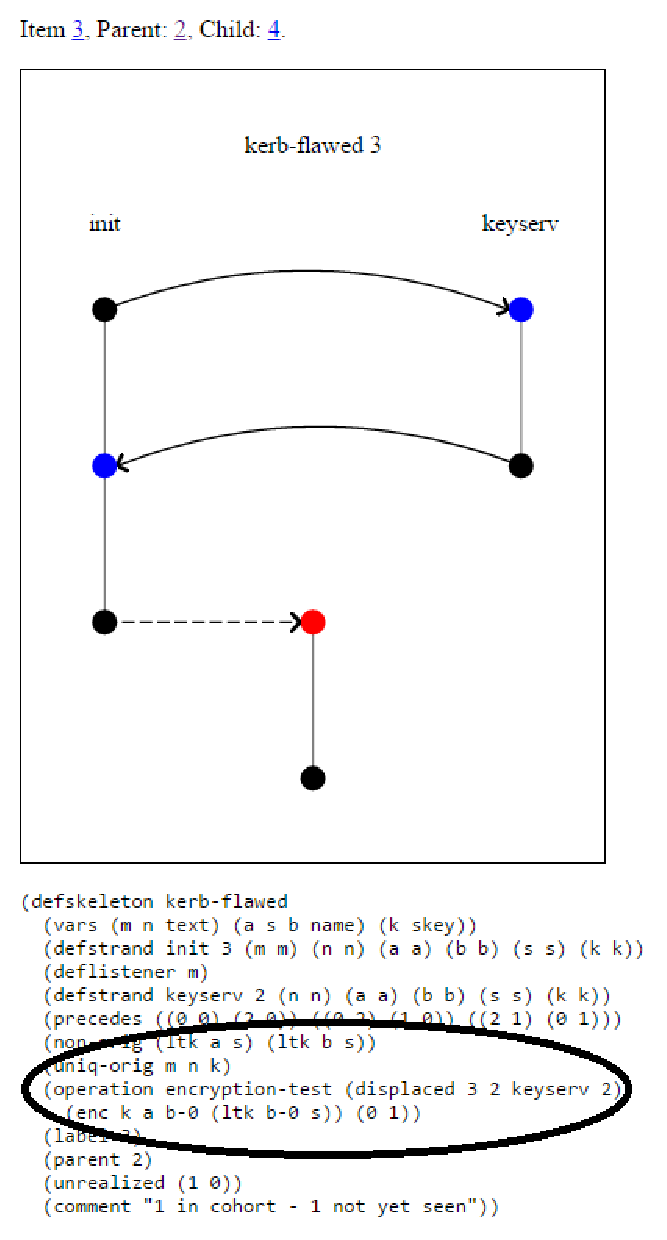
\includegraphics[scale=0.8]{kerb_skel3_operation_circled}
\end{center}
\caption{Flawed Kerberos key moment in analysis}
\label{fig:kerb-skel3}
\end{figure}

The operation field of Item 3 is telling:

\begin{center}
\verb|(operation encryption-test (displaced 3 2 keyserv 2)|\\
\verb|        (enc k a b-0 (ltk b-0 s)) (0 1))|
\end{center}

The critical term here is the encryption $\enc{k,a,b0}{K(b0,s)}$.
Thus, the ticket portion of the initiator's reception is driving this
step in the analysis.\footnote{Note that the specific encryption
  $\enc{k,a,b0}{K(b0,s)}$ is not actually present in Item 2 or in Item
  3, it is a side effect of the internal way {\cpsa} represents
  variables and determines how to display them.  Still, only the
  ticket portion of the node \texttt{(0 1)} is of this kind of format,
  so the conclusion in the text is correct.}  After the displacement
(which, you may notice, adds no new nodes), the key server agrees with
the initiator on $b$.

In other words, the tool reasons first that the presence of the
``authenticator'' portion of the reception guarantees there is a key
server instance that believes it is responding to a request initiated
by $a$, but may or may not believe the request initiated by $a$ was
for communicating with $b$.  The ticket portion makes the guarantee,
but that's strange because the ticket is for $b$ and not $a$ to
examine.  To believe this reasoning implies that the initiator really
is checking the format of the ticket, which the analyst should realize
is not the way the protocol is intended to work.

If you next examine the properly modeled protocol, you will find that
Items 5, 6, and 7 follow a very similar path.  Item 6 makes Item 5 into
a skeleton, while Item 7 adds a key server instance in which the key
server agrees with the initiator on $a$ but not on $b$.  But Item 7 is
a realized skeleton, while Item 2 is not realized.

%%% Local Variables:
%%% mode: latex
%%% TeX-master: "cpsa4manual"
%%% End:

\chapter{Constraining CPSA's search}
\label{ch:declarations}

If you have read Chapters~\ref{ch:basic} and~\ref{ch:algebra}, you
have seen the \texttt{uniq-orig} and \texttt{non-orig} features, which
are the first representatives of a large class of features called
\emph{declarations}.  These ``declare'' certain assumed properties about
an execution in order to constrain the tool's search.  In this chapter,
we will describe more precisely the notion of execution that motivates
the {\cpsa} analysis, and precisely define these and other declarations
available for use in the tool.

\section{Bundles: A Strand-Based Execution Model}
\label{sec:bundles}

\index{strand spaces} \index{event} The {\cpsa} tool is based on
strand space theory~\cite{DoghmiGuttmanThayer07}.  A strand is simply
a sequence of \emph{events}, which are transmissions or receptions of
messages.

A bundle is a set of strands, along with a satisfaction relation
$\rightarrow$ from transmissions to receptions, where for every
reception event $e_1$ of a message $m$, there is a unique transmission
event $e_0$ of $m$ such that $e_0 \rightarrow e_1$, and such that the
graph formed on the events of the strands with edges defined by
$\rightarrow$ and strand succession is acyclic.

Bundles express an explanatory framework in which a set of sequential
viewpoints of transmissions and receptions is self-contained.  Although
bundles do not totally order the events, they express the orderings that
are essential due to causality.

The most basic notion of a protocol is simply a set of roles which are
each themselves strands representing a template of behavior.  A bundle
is a bundle \emph{of a protocol} $P$ if every strand in the bundle is
either an instance of a role in $P$ or an instance of a penetrator
role.  There are two types of penetrator roles: derivation roles and
the ``create'' role.  The derivation roles are determined by the
message model; one matches each derivability rule in the algebra used.
The create role consists of a one-event strand in which certain basic
values may be transmitted.  This always includes all constants (such
as tag constants or the generator $g$ in the Diffie-Hellman algebra),
and also includes all values of basic sorts: the sorts other than
$\scap{mesg}$ in the basic algebra, and those sorts plus the
$\scap{rndx}$ sort in the Diffie-Hellman algebra.

\section{Secrecy assumptions}
\label{sec:secrecy_assumptions}
A priori, the analysis of (say) the initiator's point of view in
Needham-Schroeder is tasked with exploring all bundles of the
Needham-Schroeder protocol in which an initiator instance of
sufficient length is included.  As it turns out, there is a most
general shape, namely, the full-length initiator instance, alone.
However, the bundle this shape describes is not of great interest,
because the nonce chosen by the initiator appears in a ``create''
instance.

An assumption of secrecy is, in essence, a statement that the analyst
is interested only in certain bundles.  In the case of this nonce, for
instance, we assume the nonce is secret and are thus uninterested in
bundles in which that nonce appears in a ``create'' instance.

There are four declarations that may be used in {\cpsa} to represent
a secrecy assumption, but these assumptions are distinct from each other
and each have a particular semantic and syntactic meaning.

\index{carried subterm}
To describe these assumptions, we first need some terminology.  We
use ``carried'' to refer to subterms of a term that can potentially be
obtained from that term via decomposition. A pair carries each of its
elements, and an encryption carries its plaintext.  We extend this
notion transitively, so for instance $\enc{n1, n2}{K(a)}$ carries $n1$
since it carries the plaintext $(n1, n2)$ which in turn carries $n1$.

\index{origination} We say that a value \emph{originates} on a strand
when its first \emph{carried} occurrence is in a transmission.
\index{generation} We say that a value \emph{generates} on a strand
when its first occurrence (whether carried or not) in that strand is
in a transmission.

\begin{itemize}
\index{origination!unique}
\item A value \emph{uniquely originates} in a bundle if it originates
  on exactly one strand.  Note that if the unique origination point of
  a value is on a regular strand, then it cannot be produced in a
  ``create'' instance because that would constitute a second point of
  origination.

\index{origination!non-origination}
\item A value is \emph{non-originating} in a bundle if it does not
  originate on any strands.  A simple lemma can show that a value is
  non-originating only if it is not carried in any message in the
  bundle.

\index{origination!penetrator non-origination}
\item A value is \emph{penetrator non-originating} in a bundle of
  a protocol if it does not originate on any penetrator strands.
  Clearly, such a value cannot be produced in a ``create'' instance.
\end{itemize}

\ttindex{uniq-orig} \ttindex{non-orig} \ttindex{pen-non-orig} The
presence of a \texttt{uniq-orig}, \texttt{non-orig}, or
\texttt{pen-non-orig} declaration of a value is a statement by the
user that they are only interested in bundles in which the declared
value uniquely originates, is non-originating, or is penetrator
non-originating, respectively.

\ttindex{uniq-gen} The fourth declaration that imposes a secrecy
assumption is the \texttt{uniq-gen} declaration.  The presence of a
\texttt{uniq-gen} declaration of a value equates to a restriction to
bundles in which the declared value generates on only one strand.
Note that if a value that generates uniquely generates on a regular
strand, it cannot be produced in a ``create'' instance.

The \texttt{uniq-orig} (resp. \texttt{uniq-gen}) declaration can only
be used in {\cpsa} input for values that do originate (resp. generate)
on the role or in the skeleton in which the declaration appears.  This
forces the use of such declarations to create a secrecy assumption.

Because ``generation'' covers a wider set of occurrences than
``origination,'' a value that originates uniquely on one strand may
still generate on a different strand.  For instance, it may be used to
encrypt a message on that strand.  This means that one can model a key
(for instance) that is distributed from a point of unique origination,
and subsequently used to encrypt messages on other strands, without
modeling a particular mechanism for storing it in the recipient's
device.  This property of origination and generation can, however,
cause surprises if the key could surface unexpectedly in other
strands.  See Chapter~\ref{chap:channels:state} to understand how to
store values explicitly, when that is desired.

In fact, because ``generation'' covers a wider set of occurrences than
``origination,'' when a value $v$ originates on a strand, declaring
$v$ \texttt{uniq-gen} is actually stronger than declaring it
\texttt{uniq-orig}.  The \texttt{uniq-gen} declaration prohibits
unexplained key usage, as opposed to the \texttt{uniq-orig}
declaration that permits it.  

\begin{exercise}
Experiment with variants of your favorite simple protocol in which you
try replacing \texttt{uniq-orig} with \texttt{uniq-gen} and/or
\texttt{non-orig} with \texttt{pen-non-orig}.  What do you find?
\end{exercise}

\begin{exercise}
Suppose a protocol you wish to model involves key management, and
includes keys being encrypted and transmitted and received in
encrypted form.  What declaration should you use to model a long-term
(not recently chosen) key as secret, if you are concerned about the
actual possibility of that key leaking?
\end{exercise}

Note: these four declarations (\texttt{uniq-orig, non-orig,
  pen-non-orig,} and \texttt{uniq-gen}) may only be applied to basic
values.  One of the main purposes of such declarations is to restrict
the use of the ``create'' role in bundles, so such declarations on
values that cannot be produced in the ``create'' role is undesirable.

\section{Diffie-Hellman declarations}
A declaration arises as a part of the algorithm {\cpsa} uses for
Diffie-Hellman protocols.  Like other declarations, these may be
provided as part of a protocol or skeleton input.

\begin{itemize}

  \item \ttindex{absent} The \texttt{absent} declaration specifies
    that a particular \scap{rndx} variable does not occur in a base or
    exponent expression.  This declaration is automatically added to
    specify $x$ is absent within $y$ whenever $y$ is a base or
    exponent expression that occurs in a strand in which $x$ is
    declared \texttt{uniq-gen} before the point where $x$ is
    generated.  This declaration is also added by the algorithm in
    rare circumstances.
%z
\end{itemize}

\iffalse

\section{Distinctness assumptions}
\label{sec:distinct_decls}

\index{inequality declarations}
\index{distinctness declarations}
One inconvenient consequence of representing protocol roles as strands
is that certain kinds of checks are not easy to represent.  The
structure of received terms implies that the participant executing the
protocol is capable of parsing and checking such formats.  However,
there is no way, with format, to represent a check that two values are
unequal.

The tool includes four special declarations that may be used to
describe distinctness of values.

\begin{itemize}

\ttindex{neq}
\item A pair of values may be declared unequal with the \texttt{neq}
  declaration.  For instance, \texttt{(neq (a b))} restricts the
  analysis to consider bundles in which $a \neq b$.  See
  \texttt{neq\_test.scm} in the examples directory for examples of use.

\ttindex{neqlist}
\item A larger list of values may be declared distinct with the
  \texttt{neqlist} declaration.  For instance, \texttt{(neqlist (a b c
    d))} adds a requirement that $a, b, c$, and $d$ all be distinct
  from one another.  This may be useful as shorthand, rather than the more
  cumbersome \texttt{(neq (a b) (a c) (a d) (b c) (b d) (c d))}.

\ttindex{subsort}
\item The $\scap{data}$ and $\scap{text}$ sorts are identical to one
  another, but they are distinct and thus allow a user to separate the
  purpose of certain parameters from others, and exclude analyses in
  which parameters are confused across types.  The \texttt{subsort}
  declaration may be used to sub-categorize values into disjoint
  classes, which may never be confused for each other.  For instance,
  an e-commerce protocol may involve prices, quantities, item numbers,
  et cetera.  Each subsort is named with a string.  For instance,
  \texttt{(subsort ("A" a1 a2 a3) ("B" b1 b2))} defines two classes of
  values, ``A'' and ``B'', and requires that no ``A'' value be equal
  to any other value with a subsort other than ``A''.  So in
  particular, all the $a$ variables are distinct from the $b$
  variables and vice versa, but the $a$ variables are not required to
  be distinct from each other.  See \texttt{subsort\_test.scm} in the
  examples directory for examples of use.

\ttindex{lt}
\item Finally, one particular reason two values may be unequal is if
  they are compared and put in an order.  For instance, in an auction,
  a bid may be rejected only if another bid is strictly higher.  Or, a
  value in a protocol model may be intended to represent time, and
  some of these may be strictly orderable with respect to each other.
  The \texttt{lt} declaration (short for ``less than'') asserts a
  strict comparability between two values in a partial order.  For
  instance, \texttt{(lt (a b))} declares that $b$ is less than $a$.
  The presence of \texttt{lt} declarations on pairs of values
  restricts the tool to bundles in which the implied orderings form no
  cycles.  See \texttt{lt\_test.scm} in the examples directory for
  examples of use.
\end{itemize}

For each of these declarations, {\cpsa} checks the conditions required
at every skeleton it considers.  Those skeletons for which any
required condition is violated are discarded.  You will never see a
skeleton with (for instance) \texttt{(neq (a a))} in it.

\section{Functional dependence assumptions}

Another disadvantage of the lightweight way {\cpsa} represents
protocols is that it does not understand the relationships between
values involved in messages.  For instance, an e-commerce protocol
may involve both identifiers for merchandise and prices.  An honest
merchant would assign a consistent price to any particular item,
but protocol roles and secrecy or distinctness assumptions cannot
describe this particular scenario.

\ttindex{fn-of} \index{functional dependence}
For this purpose, {\cpsa} allows the declaration of a functional
dependence using the \texttt{fn-of} declaration (short for ``function
of'').  Like the \texttt{subsort} declaration, a subtag is required
to identify the function, so that multiple independent functions could
be described if necessary.  An example:

\begin{center}
\verb|(fn-of ("f" (y x) (z w)))|
\end{center}

This declaration says that there is a function $f$ such that $y=f(x)$
and $z=f(w)$.  In the e-commerce example, if $f$ was the ``price of''
function, then $x$ and $w$ would be items and $y$ and $z$ would be
their respective prices.  The presence of a set of \texttt{fn-of}
declarations restricts the tool's search so that in this case, if
$x = w$ then $y = z$.

\index{Yahalom protocol}\index{examples!Yahalom}
The \texttt{fn-of} declaration is a powerful tool that can emulate
function symbols in the algebra.  See \texttt{yahalom.scm} in the
examples repository for an example protocol involving the \texttt{ltk}
function symbol.  We can totally emulate the use of this function symbol
via the \texttt{fn-of} declaration: see \texttt{fnof\_yahalom.scm} for how
this is done.

\index{init@\texttt{init}!use for introducing variables} It is important to note
that one limitation of the \texttt{fn-of} declaration is that it
cannot introduce variables not used in a skeleton or role.  The
emulation of the \texttt{ltk} symbol in \texttt{fnof\_yahalom.scm}, for
instance, requires three variables (the long-term key variable and the
two names) where there were formerly only two.  {\cpsa} will ignore
declarations involving variables not present anywhere, so in order to
make sure these declarations are not ignored, we need to use the
variables in the trace.  We use the \texttt{init} event (see
Chapter~\ref{chap:channels:state}) to introduce these variables, since we know
that without state events this will have no effect on the penetrator's
abilities.

\subsection{Equality constraints}

\index{equality} \ttindex{eq} The \texttt{fn-of} declaration allows a
user to express functional dependence relationships between values.
In simpler inputs, it may be desirable to simply declare that two
values are equal; this is particularly useful for Diffie-Hellman
protocols, for instance, to declare that two separate parties agree on
a session key.  The \texttt{eq} declaration simply declares that two
values must be equal.  An example:

\begin{center}
  \verb|(eq ((exp (gen) (mul x y)) (exp (gen) (mul z w))))|
\end{center}

This declaration guarantees that $g^{xy} = g^{zw}$.

\section{Role declarations and conditional role declarations}
\label{sec:role_decls2}

\index{role declarations} When a declaration is present in a
\texttt{defskeleton} in an input file, the constraint is applied to
all analyses that descends from that skeleton.  In
Section~\ref{sec:blanchet} we discussed the notion of a role
declaration and how such a declaration differs in meaning from a
skeleton declaration.

Here we discuss more precisely when a role declaration affects a
skeleton.  Skeletons are made up of \emph{instances}, which follow
the structure of a role, but instances do not have to be full-length.
The declarations inherited in an instance of a role from the role
may vary based on the length of the instance.

Declarations are, most importantly, declarations on a term or list of
terms.  A declaration is not inherited in an instance of height $h$
(that is, an instance of the first $h$ events in the role) unless all the
variables present in terms in the declaration are present in the first $h$
events in the role's trace.

The tool also regards declarations as about a node or list of nodes,
although in most cases that list is empty.  There are two exceptions.
\ttindex{uniq-gen} \ttindex{uniq-orig} The \texttt{uniq-gen} and
\texttt{uniq-orig} declarations refer to the node at which the
declared value generates or originates, but in an automatic and
hidden way.

Role declarations refer to a node which is a particular event in the
role's trace.  In addition to the rule about variables in a
declaration's terms, a declaration is only inherited if all its nodes
are present in the instance.

\index{role declarations!conditional} All the declarations natively
included in the tool may include a node when used in a role.  This
allows the user to describe declarations that are conditional on
sufficient progress being made through the role's trace.  This may
be appropriate when, for instance, a participant receives a certificate
and comes to trust a party it has already started communicating with.

A declaration is made conditional by replacing a term (or list of
terms) with a list whose first element is the term (or list of terms)
and whose second element is the node.  Most {\cpsa} declarations allow
many declarations to be made in one S-expression; for instance
\texttt{(non-orig k1 k2 k3)} is actually three distinct declarations
rather than one.  To make the $k1$ declaration conditional on reaching
node 3, we would write \texttt{(non-orig (k1 2) k2 k3)}.  See
Table~\ref{tab:decl_syntax} for full detail on the syntax for
conditional declarations.

\section{Diffie-Hellman declarations}
There are two declarations that arise as a part of the algorithm
{\cpsa} uses for Diffie-Hellman protocols.  Like other declarations,
these may also be provided as part of a protocol or skeleton input.

\begin{itemize}

  \item \ttindex{absent} The \texttt{absent} declaration specifies
    that a particular \scap{rndx} variable does not occur in a base or
    exponent expression.  This declaration is automatically added to
    specify $x$ is absent within $y$ whenever $y$ is a base or
    exponent expression that occurs in a strand in which $x$ is
    declared \texttt{uniq-gen} before the point where $x$ is
    generated.  This declaration is also added by the algorithm in
    rare circumstances.

  \item \ttindex{precur} The \texttt{precur} declaration specifies
    that a particular node is present in the skeleton to be the
    ``precursor'' for some other value.  This is used to prevent
    {\cpsa} from failing to terminate in certain cases.
\end{itemize}

\section{Other declarations}
\label{sec:other_decls}

The tool makes use of declaration-like syntax for several other
purposes.

\paragraph{Precedes.}
\ttindex{precedes} In {\cpsa} text output, you may notice an
S-expression that starts with \texttt{precedes}.  This is how {\cpsa}
records the orderings present in a skeleton, before it is graphed.
You may also use precedes declarations within a \texttt{defskeleton},
to set up orderings between strands.

\ttindex{leadsto}
\paragraph{Leadsto.}  Similarly, the \texttt{leadsto} field of
a \texttt{defskeleton} specifies state causality orderings.  See
Chapter~\ref{chap:channels:state} for more detail on what this means.

\paragraph{Priority.}
\ttindex{priority} The tool contains an ability to declare a priority
for certain receptions that differs from the default.  Priority takes
precedence over all other search orderings.  See
Section~\ref{sec:decl_syntax} for the format requirements for
declaring priorities, and the \texttt{priority\_test.scm} example in the
examples directory.

Note that the default priority is 5, and priority 0 indicates that the
tool should never bother solving tests at those nodes.  This may be of
use, for instance, if solving one particular node leads to infinite
analysis, but other nodes would result in a quick determination that a
skeleton is dead.

\paragraph{User-defined declarations.}
The final type of declaration supported by {\cpsa} is totally general,
but does not affect the search.  Instead, this type of declaration is
merely kept around as a note about the skeleton in question, but a
note that is aware of its use of algebra variables and nodes and
evolves as the skeleton evolves.

\index{user-defined declarations} \ttindex{decl} This feature is meant
for advanced users only, who may wish to write their own custom
post-processing tools.  For this reason we do not give an example
involving user-defined declarations; for the proper syntax, consult
Table~\ref{tab:decl_syntax}.  The keyword to identify a user-defined
declaration is \texttt{decl}.

\fi

\section{A Caution about typos}
Declarations are typically found syntactically in ``association
lists'' which include declarations and may also include other fields,
whether in protocol declarations, role declarations within them, or in
skeleton query declarations.  For instance, the {\cpsa} tool creates
associations in its \texttt{defskeleton} outputs specifying things
like the algorithmic method used to produce this skeleton, or the
label of the parent, etc.  {\cpsa} handles comments in the same way.
Any association list entry \verb|(header| \dots
\emph{stuff}\dots\verb|)| in which the header is unrecognized is
treated as a comment, and preserved in the output.  This is convenient
not just for documenting your specifications, but also for defining
material to be used not by {\cpsa} itself but by downstream tools.

Be careful when using declarations that you do not mis-spell the
keywords!  If you do, they will typically be treated just like a
comment and ignored, so they will not have the effect you intended.

%%% Local Variables:
%%% mode: latex
%%% TeX-master: "cpsa4manual"
%%% End:

\part{Advanced features of CPSA}
\label{part:advanced}
\chapter{Logical Security Goals and Rules}
\label{ch:goals}

\newtheorem{axiom}{Trust Assumption}

How easy is it to read off authentication and secrecy properties?
What precisely is it that an expert sees?  This chapter describes
{\cpsa}'s support for reasoning about security goals using first-order
logic.  With security goals expressed in first-order logic, intuition
is replaced by determining if a formula is true in all executions of
the protocol.

% \emph{Something about the benefits of first-order logic goes here.}

This treatment of security goals relies heavily on a branch of
first-order logic called model theory.  It deals with the relationship
between descriptions in first-order languages and the structures that
satisfy these descriptions.  In our case, the structures are skeletons
that denote a collection of executions of a protocol.  This chapter
describes the language of security goals and its structures without
requiring the reader to have studied model theory.

The model theoretical foundation of this approach to security goals
appears in~\cite{Guttman14}.  A practical use of security goals in
protocol standardization is described
in~\cite{guttman2014security,RoweEtAl2016}.  The precise semantics of
the goal language is in~\cite{Ramsdell12}.  The syntax of
security goals appears in Table~\ref{tab:goal_syntax}.

\begin{table}
\begin{center}\scshape
  \begin{tabular}{rcl}
 goal&$\leftarrow$&(\sym{defgoal} id sentence+ alist)
\\ sentence&$\leftarrow$&(\sym{forall} (gvdecl$\ast$) implication)
\\ gvdecl&$\leftarrow$&(id+ sort)~$\mid$~(id+ \sym{strd})~$\mid$~(id+ \sym{indx})
\\ implication&$\leftarrow$&(\sym{implies} conjunction conclusion)
\\ conjunction&$\leftarrow$&atomic~$\mid$~(\sym{and} atomic+)
\\ conclusion&$\leftarrow$&(\sym{false})~$\mid$~existential
\\ &$\mid$& (\sym{or} existential+)
\\ existential&$\leftarrow$&conjunction~$\mid$~(\sym{exists} (gvdecl$\ast$) conjunction)
\\ atomic&$\leftarrow$&(\sym{p} string strdvar integer)
\\ &$\mid$&(\sym{p} string string strdvar term)
\\ &$\mid$&(\sym{prec} strdvar index strdvar index)
\\ &$\mid$&(\sym{leads-to} strdvar index strdvar index)
\\ &$\mid$&(\sym{non} term)~$\mid$~(\sym{pnon} term)
\\ &$\mid$&(\sym{uniq} term)~$\mid$~(\sym{uniq-at} term strdvar index)
\\ &$\mid$&(\sym{ugen} term)~$\mid$~(\sym{ugen-at} term strdvar index)
\\ &$\mid$&(\sym{=} strdvar strdvar)~$\mid$~(\sym{=} term term)
    \\ &$\mid$&(\sym{fact} id term*)
                %~$\mid$~(\sym{absent} (term term)+)
\\ strdvar&$\leftarrow$&symbol
\\ index&$\leftarrow$&symbol~$\mid$~integer
  \end{tabular}
\end{center}
\caption[Goal syntax]{Goal syntax.  See Tables~\ref{tab:basic_term}
  and~\ref{tab:dh_term} for the algebra syntax, which defines the
  $\scap{term}$ and $\scap{sort}$ symbols.}
\label{tab:goal_syntax}
\end{table}

\ttindex{defgoal}\ttindex{forall}\ttindex{implies}\ttindex{false}\ttindex{exists}
\ttindex{and}\ttindex{or}

The {\cpsa} distribution contains, in its examples directory, the
input file \texttt{goals.scm}.  The reader is encouraged to run the
examples and examine the output while reading this chapter.

%% Use a margin width of 62 for S-expressions

\begin{figure}
\begin{center}
\includegraphics{cpsadiagrams-0.mps}\hfil
\includegraphics{cpsadiagrams-1.mps}\\
\end{center}
\begin{center}
\begin{minipage}{3in}
\begin{verbatim}
(defprotocol ns basic
  (defrole init
    (vars (a b name) (n1 n2 text))
    (trace
     (send (enc n1 a (pubk b)))
     (recv (enc n1 n2 (pubk a)))
     (send (enc n2 (pubk b)))))
  (defrole resp
    (vars (b a name) (n2 n1 text))
    (trace
     (recv (enc n1 a (pubk b)))
     (send (enc n1 n2 (pubk a)))
     (recv (enc n2 (pubk b))))))
\end{verbatim}
\end{minipage}
\end{center}
\caption{Needham-Schroeder Initiator and Responder Roles}
\label{fig:ns roles 2}
\end{figure}

\begin{figure}
\begin{verbatim}
(defgoal ns                ; Goal
  (forall ((b name) (n1 text) (z0 strd))
    (implies
     (and (p "init" z0 3)
      (p "init" "n1" z0 n1) (p "init" "b" z0 b)
      (non (privk b)) (uniq n1))
     (exists ((z1 node))
      (and (p "resp" z1 2) (p "resp" "b" z1 b))))))

(defskeleton ns            ; Point of view skeleton
  (vars (a b name) (n1 n2 text))
  (defstrand init 3 (a a) (b b) (n1 n1) (n2 n2))
  (non-orig (privk b))
  (uniq-orig n1))
\end{verbatim}
{\centering
\includegraphics{cpsadiagrams-9.mps}}
\begin{verbatim}
(defskeleton ns            ; Shape
  (vars (n1 n2 text) (a b name))
  (defstrand init 3 (n1 n1) (n2 n2) (a a) (b b))
  (defstrand resp 2 (n2 n2-0) (n1 n1) (b b) (a a))
  (precedes ((0 0) (1 0)) ((1 1) (0 1)))
  (non-orig (privk b))
  (uniq-orig n1)
  (satisfies yes))
\end{verbatim}
\caption{Needham-Schroeder Initiator Point of View}
\label{fig:ns init}
\end{figure}

\index{Needham-Schroeder!logical goals in}
\index{examples!Needham-Schroeder!logical goals in}
In this chapter we return to the Needham-Schroeder protocol discussed
in Chapter~\ref{ch:basic}.  The roles are displayed in
Figure~\ref{fig:ns roles 2}.

The protocol is analyzed from the point of view of a complete run of
one instance of the initiator role.  The input security goal, followed
by the point of view skeleton it generates and the shape produced by
{\cpsa}, are shown in Figure~\ref{fig:ns init}.  The syntax and
semantics of the goal will be explained later.  Roughly speaking, it
asserts that if a realized skeleton contains a full length initiator
strand, its private key is uncompromised, and it uniquely generates
\texttt{n1}, then the skeleton will contain a responder strand that
agrees with the initiator on the name \texttt{b}.  The shape produced
by {\cpsa} contains the annotation \texttt{(satisfies yes)}.  This
indicates that its structure satisfies the description given by the
security goal.  It will be explained later why the properties of
{\cpsa} allows us to conclude that this goal is true in all executions
of the protocol, and therefore conclude that the Needham-Schroeder
protocol achieves this authentication goal.

\section{Overview}\label{sec:goalsoverview}

In addition to \texttt{defskeleton} S-expressions, a {\cpsa} input
file may contain \texttt{defgoal} S-expressions.  Like a
\texttt{defskeleton}, a \texttt{defgoal} takes as its first parameter
the name of a protocol which the tool expects has been previously
defined in the input file.  The second parameter to a \texttt{defgoal}
is a \emph{geometric} sentence in first-order logic.  A geometric
sentence contains one implication.  The antecedent is a conjunction
of atomic formulas.  The free variables that occur in the antecedent
are universally quantified.  The conclusion is a disjunction of
existentially quantified conjunctions of atomic formulas.

Alternately, a \texttt{defskeleton} can be augmentend with a
\texttt{goal}, which may specify one or more geometric
formulas to check.

When the tool is run, a \texttt{defgoal} is converted to a
\texttt{defskeleton} that represents as narrowly as possible the
left-hand side of the implication and has a \texttt{goal} recorded for
the right-hand side.  The tool then analyzes \texttt{defskeleton}s as
usual, but realized skeletons found during the course of analysis of a
\texttt{defskeleton} with a \texttt{goal} are augmented with
a \texttt{satisfies} S-expression indicating whether the goal is met or
not.

The tool \texttt{cpsagoalsat} will examine the output from a {\cpsa}
run, and, for each goal formula, will determine whether the analysis
ensures that the goal is met.  If not, it identifies the labels of all
the skeletons that furnish counterexamples to the goal.  See
Section~\ref{ch:tools}.

The remainder of this chapter is devoted to explaining the semantics
of this feature in greater detail.

\section{Semantics}\label{sec:semantics}

In a \texttt{defgoal} sentence, the antecedent specifies the point of
view skeleton.  We focus on the antecedent.  In the example,

\begin{quote}
\begin{verbatim}
(defstrand init 3 (a a) (b b) (n1 n1) (n2 n2))
\end{verbatim}
\end{quote}
is extracted from
\begin{quote}
\begin{verbatim}
(and (p "init" z0 3)
  (p "init" "n1" z0 n1) (p "init" "b" z0 b)).
\end{verbatim}
\end{quote}
Notice that {\cpsa} adds a binding for \texttt{a} and \texttt{n2} just
as it does had
\begin{quote}
\begin{verbatim}
(defstrand init 3 (b b) (n1 n1))
\end{verbatim}
\end{quote}
been given as input.

Our aim now is to specify how to decide if a security goal is true in
all possible executions of a protocol.  A skeleton defines a set of
executions that contain the skeleton's structure.  We say a skeleton
\emph{satisfies} a formula if the skeleton contains all of the
structure specified by the formula.  To decide if a skeleton
satisfies a formula, we decide if it satisfies each of its atomic
formulas, and combine the results using the rules of first-order
logic.

Atomic formula \texttt{(p "init" z0 3)} is called a role strand length
formula.  A skeleton~$k$ satisfies the formula if \texttt{z0} maps to
a strand~$s$ in~$k$ such that
\begin{enumerate}
\item the trace of strand~$s$ in~$k$ has a length greater than 2, and
\item the trace when truncated to length 3 is an instance of the init
  role.
\end{enumerate}
Consider the shape in Figure~\ref{fig:ns init}.  It satisfies
\texttt{(p "init" z0 3)} when \texttt{z0} maps to~0.

Atomic formula \texttt{(p "init" "n1" z0 n1)} is called a role
parameter formula.  A skeleton~$k$ satisfies the formula if
\texttt{z0} maps to strand~$s$ in~$k$, \texttt{n1} first occurs in at
position~$i$ in the trace of the init role, and \texttt{n1} maps to a
message algebra term~$t$ in~$k$ such that
\begin{enumerate}
\item the trace of strand~$s$ in~$k$ has a length greater than~$i$,
\item the trace truncated to length $i+1$ is an instance of the
  init role, and
\item the truncated trace is compatible with mapping the init role's
  \texttt{"n1"} role variable to~$t$.
\end{enumerate}
The shape in Figure~\ref{fig:ns init} satisfies \texttt{(p "init" "n1"
  z0 n1)} when \texttt{z0} maps to~0 and \texttt{n1} maps to the
message algebra term \texttt{n1}.

Collectively, a skeleton satisfies the formula
\begin{quote}
\begin{verbatim}
(and (p "init" z0 3)
     (p "init" "a" z0 a) (p "init" "b" z0 b)
     (p "init" "n1" z0 n1) (p "init" "n2" z0 n2))
\end{verbatim}
\end{quote}
if the skeleton contains the structure specified by
\begin{quote}
\begin{verbatim}
(defstrand init 3 (a a) (b b) (n1 n1) (n2 n2)).
\end{verbatim}
\end{quote}

The antecedent in Figure~\ref{fig:ns init} contains two origination
assertions.  The formula \texttt{(non (privk b))} is extracted as
\texttt{(privk b)}.  A skeleton~$k$ satisfies the formula if
\texttt{b} maps to a message algebra term~$t$ in~$k$ such that~$k$
assumes that~$t$ is non-originating.  The unique origination formula for
\texttt{n1} is similarly extracted.

Putting it all together, the mapping
\[\{\mathtt{n1}\mapsto\mathtt{n1},
\mathtt{n2}\mapsto\mathtt{n2}, \mathtt{a}\mapsto\mathtt{a},
\mathtt{b}\mapsto\mathtt{b},\mbox{\tt z0}\mapsto0\}\] shows that
the shape in Figure~\ref{fig:ns init} satisfies the antecedent of the
security goal.

The \texttt{prec} predicate is used to assert a node precedes another
node.  The conclusion in Figure~\ref{fig:ns init} with \texttt{(prec
  z1 1 z0 2)} added is satisfied by the shape using the mapping
$\mbox{\tt z0}\mapsto0$ and $\mbox{\tt z1}\mapsto1$.

The \texttt{uniq-at} predicate is used to assert not only that an atom
uniquely originates, but also the node at which it originates.  In the
Figure~\ref{fig:ns init} goal, the \texttt{(uniq n1)} formula could
have been replaced by \texttt{(uniq-at n1 z0 0)}.  The extracted point
of view skeleton is the same.

The \texttt{ugen} and \texttt{ugen-at} predicates are similar, except
that they refer to an earliest outbound occurrence, whether carried or
not.  If an atom is an asymmetric key, it and its inverse are
generated together at the first outbound occurrence of either one.

\iffalse{
    %
    In the Diffie-Hellman algebra (see Section~\ref{sec:input:dh}), a
    random exponent $x\colon\sym{rndx}$ is \texttt{absent} from a term
    $t\colon\sym{expt}$ if the latter is a monomial in which $x$ is of
    degree 0.  Homomorphisms must preserve this positive formula,
    meaning that, given a skeleton satisfying
    $\texttt{absent}(x,\alpha)$, a map such as $\alpha\mapsto xy$ is
    not a homomorphism instantiating $\alpha$.  It would map $\alpha$
    to a monomial in which $x$ has degree 1.  }
  %
\fi

Recall that our aim in analyzing a protocol is to find out what
security goals are true in all of its possible executions.  We are
interested in runs of {\cpsa} that show that when every shape
satisfies a goal, it is true in every execution.

When {\cpsa} performs a shape analysis, every shape it generates
refines the input skeleton.  Skeleton refinement is defined
in~Chapter~\ref{ch:algorithm}.  The definition makes precise the
notion of structure containment, as skeleton~$A$ refines skeleton~$B$
if and only if~$A$ contains the structure of skeleton~$B$.

The skeleton~$k_0$ extracted from the antecedent of a security goal
has the property that a skeleton refines~$k_0$ if and only if it
satisfies the antecedent.  A skeleton with this property is called the
\emph{characteristic skeleton} of the antecedent.

Given a goal~\(\Phi\), consider a shape analysis starting from the
characteristic skeleton~$k_0$ of its antecedent.  Assume {\cpsa} finds
shapes $k_1,\ldots,k_n$ and that {\cpsa} determines that each~$k_i$
satisfies~$\Phi$.  Consider the executions that contain the structure
in~$k_0$.  {\cpsa} tells us that each execution is in the executions
that contain the structure of some~$k_i$.  Furthermore, because~$k_0$
is a characteristic skeleton, each~$k_i$ satisfies the antecedent
of~$\Phi$.  Executions that do not contain the structure in~$k_0$ do
not satisfy the antecedent.  Therefore,~$\Phi$ is true in all
executions of the protocol and maximally informative.

\section{Examples}\label{sec:examples}

This section contains examples of both authentication and secrecy
goals.  The first example shows the feedback the user receives when a
shape does not satisfy a security goal.  The second example shows how
to use a listener to state a secrecy goal.

\subsection{Needham-Schroeder Responder}\label{sec:ns resp}

\begin{figure}
\begin{verbatim}
(defgoal ns                ; Goal
  (forall ((a b name) (n2 text) (z0 strd))
    (implies
      (and (p "resp" z0 3) (p "resp" "n2" z0 n2)
        (p "resp" "a" z0 a) (p "resp" "b" z0 b)
        (non (privk a)) (uniq n2))
      (exists ((z1 strd))
        (and (p "init" z1 2) (p "init" "b" z1 b))))))

(defskeleton ns            ; Point of view skeleton
  (vars (a b name) (n1 n2 text))
  (defstrand resp 3 (a a) (b b) (n1 n1) (n2 n2))
  (non-orig (privk a))
  (uniq-orig n2))
\end{verbatim}
\begin{center}
\includegraphics{cpsadiagrams-10.mps}
\end{center}
\begin{verbatim}
(defskeleton ns            ; Shape
  (vars (n1 n2 text) (a b b-0 name))
  (defstrand resp 3 (n2 n2) (n1 n1) (b b) (a a))
  (defstrand init 3 (n1 n1) (n2 n2) (a a) (b b-0))
  (precedes ((0 1) (1 1)) ((1 2) (0 2)))
  (non-orig (privk a))
  (uniq-orig n2)
  (satisfies (no (a a) (b b) (n2 n2) (z0 0))))
\end{verbatim}
\caption{Needham-Schroeder Responder Point of View}
\label{fig:ns resp}
\end{figure}

Figure~\ref{fig:ns resp} contains an analysis of Needham-Schroeder
from the point of view of a complete run of the responder under the
assumption that the responder's private key is uncompromised and the
nonce it generates uniquely originates.

The conclusion of the goal asserts that in an execution compatible
with the point of view, there must be an initiator strand that agrees
with the responder strand on the name \texttt{b}.  The shape produced
by {\cpsa} is a counterexample to this assertion.  Because of this,
{\cpsa} annotates the shape with
\begin{quote}
\begin{verbatim}
(satisfies (no (a a) (b b) (n2 n2) (z0 0))).
\end{verbatim}
\end{quote}
The annotation includes a variable mapping for the shape that
satisfies the antecedent of the goal but does not satisfy its
conclusion.  The reason the shape does not satisfy the goal is because
the mapping \texttt{(b b)} maps the initiator's \texttt{b} parameter
to \texttt{b}, not \texttt{b-0} as is required to model the shape.

Galvin Lowe identified this authentication failure in
Needham-Schroeder and provided a fix.  In the Needham-Schroeder-Lowe
Protocol, the name \texttt{b} is included within the encryption in second
message of both roles.  With this modification, the shape found by
{\cpsa} satisfies the security goal in Figure~\ref{fig:ns resp}, so
Needham-Schroeder-Lowe achieves this authentication goal.

\subsection{A Needham-Schroeder Secrecy Goal}\label{sec:secrecy goal}

\begin{figure}
\begin{quote}\small
\begin{verbatim}
(defgoal ns
  (forall ((a b name) (n1 text) (z0 z1 strd))
    (implies
      (and (p "init" z0 3) (p "init" "n1" z0 n1)
        (p "init" "a" z0 a) (p "init" "b" z0 b)
        (p "" z1 1) (p "" "x" z1 n1)  ; Listener
        (non (privk a)) (non (privk b))
        (uniq n1))
      (false))))
\end{verbatim}
\end{quote}
\caption{Needham-Schroeder Secrecy Goal}\label{fig:ns secrecy}
\end{figure}

Figure~\ref{fig:ns secrecy} contains an analysis of Needham-Schroeder
from the point of view of a complete run of the initiator under the
assumption that the responder's and its peer's private keys are
uncompromised and the nonce~\texttt{n1} it generates uniquely
originates.  Futhermore, the point of view asserts that the nonce is
leaked using a listener.
\begin{quote}
\begin{verbatim}
(p "" z1 1) (p "" "x" z1 n1)    ; Listener
\end{verbatim}
\end{quote}

{\cpsa} finds no shapes, so Needham-Schroeder achieves this secrecy
goal and does not leak~\texttt{n1}.

\section{The Rest of the Story}\label{sec:whole story}

The examples in the previous section demonstrate the typical way
security goals are analyzed with {\cpsa}.  However, there are more
features that may be useful.

A \texttt{defgoal} form may contain more than one sentence.  See
Figure~\ref{fig:ns init goals} for an example.  When presented with
more than one sentence, {\cpsa} extracts the point of view skeleton
from the first sentence.

It is wise to ensure that the antecedent in every sentence is
identical.  When {\cpsa} performs satisfaction-checking on
sentence~$\Phi$, it only determines if each shape it finds is
satisfied.  If the point of view skeleton is not the characteristic
skeleton of the antecedent of~$\Phi$, the fact that all skeletons
satisfy~$\Phi$ cannot be used to conclude that~$\Phi$ is true in all
executions of the protocol.

\begin{figure}
\begin{quote}\small
\begin{verbatim}
(defgoal ns
  (forall ((a b name) (n text) (z0 strd))
    (implies
      (and (p "init" z0 2) (p "init" "n1" z0 n)
        (p "init" "a" z0 a) (p "init" "b" z0 b)
        (non (privk a)) (non (privk b)) (uniq n))
      (exists ((z1 strd))
        (and (p "resp" z1 2) (p "resp" "b" z1 b)))))
  (forall ((a b name) (n text) (z0 strd))
    (implies
      (and (p "init" z0 2) (p "init" "n1" z0 n)
        (p "init" "a" z0 a) (p "init" "b" z0 b)
        (non (privk a)) (non (privk b)) (uniq n))
      (exists ((z1 strd))
        (and (p "resp" z1 2) (p "resp" "a" z1 a))))))
\end{verbatim}
\end{quote}
\caption{Two Initiator Authentication Goals}\label{fig:ns init goals}
\end{figure}

{\cpsa} performs satisfaction-checking when an input skeleton in annotated
with one or more security goals.  The annotation uses the
\texttt{goals} key.

\begin{quote}
  \begin{alltt}
(defskeleton
   \ldots
   (goals \textsc{sent\ensuremath{+}}))
  \end{alltt}
\end{quote}

The program \texttt{cpsasas}, discussed in the next section, can be
used to generate a formula with an antecedent such that the input
skeleton is the characteristic skeleton of the antecedent.

\subsection{Shape Analysis Sentences}\label{sec:sas}

A shape analysis sentence expresses all that can be learned from a run
of {\cpsa} as a security goal.  If a security goal can be derived from
a shape analysis sentence, then the protocol achieves the security
goal, that is, the goal is true in all executions of the protocol.

The program \texttt{cpsasas} extracts shape analysis sentences from
the output of {\cpsa}.  Consider the first example in this paper
(Figure~\ref{fig:ns init}), which is in the sample file
\texttt{goals.scm}.  To generate a maximally informative security goal
from the initiator point of view with \texttt{ghci} and
\texttt{Make.hs}, type
\begin{quote}
\begin{verbatim}
$ ghci Make.hs
*Make> sas "goals"
\end{verbatim}
\end{quote}
When using GNU make, type ``\texttt{make goals\_sas.text}''.  The
resulting shape analysis sentence is displayed in Figure~\ref{fig:ns
  sas}.

\begin{figure}\small
\begin{verbatim}
(defgoal ns
  (forall ((n1 n2 text) (b a name) (z strd))
    (implies
      (and (p "init" z 3) (p "init" "n1" z n1)
        (p "init" "n2" z n2) (p "init" "a" z a)
        (p "init" "b" z b) (non (privk b)) (uniq-at n1 z 0))
      (exists ((n2-0 text) (z-0 strd))
        (and (p "resp" z-0 2) (p "resp" "n2" z-0 n2-0)
          (p "resp" "n1" z-0 n1) (p "resp" "b" z-0 b)
          (p "resp" "a" z-0 a) (prec z 0 z-0 0)
          (prec z-0 1 z 1))))))
\end{verbatim}
\caption{Initiator Shape Analysis Sentence}\label{fig:ns sas}
\end{figure}

A shape analysis sentences asserts that either a realized skeleton
does not satisfy its antecedent or it satisfies one or more of the
disjuncts in its conclusion.  {\cpsa} has been designed so that this
assertion is true.  Therefore, every shape analysis sentence is true
in all executions.

A security goal is true in all executions if it can be derived from a
shape analysis sentence~\cite{Ramsdell12}.  In practice,
theorem-proving using shape analysis sentences is rarely employed.
It's clumsy and it requires too much expertise.  The main use of
\texttt{cpsasas} is for generating a formula that is edited to become
a desired security goal.

\section{Rules}\label{sec: rules}

Support for rules was introduced in version 3.6.0 of {\cpsa}.

Each protocol includes a small collection of rules.  A rule is a
sentence in the goal language presented in Section~\ref{sec:goalsyntax}.
Rules are defined after the roles of a protocol are defined.  The
syntax of a rule follows.

\begin{center}\scshape
  \begin{tabular}{rcl}
    rule&$\leftarrow$&(\sym{defrule} name sent comments)
  \end{tabular}
\end{center}

A rule is an axiom added to a protocol.  {\cpsa} uses the axiom as a
rewrite rule to derive zero or more new skeletons from a skeleton
produced during a step.  An example of a protocol with a rule is in
Figure~\ref{fig:doorsep} on Page~\pageref{fig:doorsep}.

The trust rule states that when CPSA finds a person strand of length
at least one, and the inverse of it's \texttt{p} parameter is
non-originating, CPSA should assume the inverse of it's \texttt{d}
parameter is non-originating.

\subsection{Facts}\label{sec:facts}
Each skeleton includes a small database of facts.  A fact is a named
relation among fact terms.  A fact term\index{fact term} is either a
strand of the skeleton or an algebra term.  A set of facts is defined
anywhere after strands are defined using the \sym{facts} form.  The
syntax of facts follows.

\begin{center}\scshape
  \begin{tabular}{rcl}
    facts&$\leftarrow$&(\sym{facts} fact$\ast$) \\
    fact&$\leftarrow$&(symbol fterm$\ast$) \\
    fterm&$\leftarrow$&mesg $\mid$ nat
  \end{tabular}
\end{center}

For example, in a skeleton, a user may want to note that strand 0 owns
the private key for~\texttt{a} by assuming.

\begin{center}
  \verb|(facts (owns 0 (privk a)))|
\end{center}

Facts are most useful when combined with rules.  Here is an example of
their combination.  Suppose a point of view skeleton has two names,
\texttt{a} and~\texttt{b}, and the problem is modeling a situation in
which the two names are known to differ.  To enforce this constraint, add
\begin{center}
  \verb|(facts (neq a b))|
\end{center}
to the point of view skeleton.  CPSA contains a rule governing
\texttt{neq} rule stating essentially:

%below, eliminates skeletons that
%violate the constraint.
\begin{quote}
\begin{verbatim}
(defrule neq
  (forall ((a mesg))
    (implies
      (fact neq a a)
      (false))))
\end{verbatim}
\end{quote}

\subsection{DoorSEP}

\begin{sloppypar}
As a motivating scenario consider the Door Simple Example Protocol
(DoorSEP), derived from an expository protocol that was designed to
have a weakness.  Despite this, the protocol achieves the needs of an
application, given a trust assumption.
\end{sloppypar}

Imagine a door~$D$ which is equipped with a badge reader, and a
person~$P$ equipped with a badge.  When the person swipes the badge,
the protocol executes.  Principals such as doors or persons are
identified by the public parts of their key pairs, with \iv{D} and
\iv{P} being the corresponding private keys.  We write \enc{M}{K} for
the encryption of message~$M$ with key~$K$.  We represent digital
signatures $\enc{M}{\iv{P}}$ as if they were the result of encrypting
with $P$'s private key.

$P$ initiates the exchange by creating a fresh symmetric key~$K$,
signing it, and sending it to the door $D$ encrypted with the door's
public key.  $D$ extracts the symmetric key after checking the
signature, freshly generates a token~$T$, and sends it---encrypted
with the symmetric key---back to $P$.  $P$ demonstrates they are
authorized to enter by decrypting the token and sending it as
plaintext to the door.  The two roles of DoorSEP are shown in
Fig.~\ref{fig:doorsep protocol}, where each vertical column displays
the behavior of one of the roles.  The {\cpsa} encoding of the roles is
in Figure~\ref{fig:doorsep}.

\begin{figure}[tb]
  \[\begin{array}[c]{rc@{\qquad\qquad}cl}
      & \mbox{person}
      &\mbox{door}
      &\\
      \begin{array}[c]{r} ~ \\ ~ \\
        \mbox{Fresh: $K$}
      \end{array}
      & \xymatrix@R=2mm@C=7em{
      \bullet\ar@{=>}[d]\ar[r]^{\enc{\enc{K}{\iv{P}}}{D}}
      &\\
      \bullet\ar@{=>}[d]& \ar[l]_{\enc{T}{K}}\\
      \bullet \ar[r]^T & }
      &
        \xymatrix@R=2mm@C=7em{
        \ar[r]^{\enc{\enc{K}{\iv{P}}}{D}}    &\bullet\ar@{=>}[d]\\
      &\bullet\ar@{=>}[d] \ar[l]_{\enc{T}{K}}\\
      \ar[r]^T      &\bullet}
      &
        \begin{array}[c]{r} ~ \\ ~ \\
          \mbox{Fresh: $T$}
        \end{array}
  \end{array}\]
  \caption{DoorSEP Protocol}\label{fig:doorsep protocol}
\end{figure}

%   \[
%   \begin{array}{l@{{}:{}}l}
%     P\to D & \enc{\enc{K}{\iv{P}}}{D}\\
%     D\to P & \enc{T}{K}\\
%     P\to D & T.
%   \end{array}
%   \]

{\cpsa} finds an undesirable execution of DoorSEP.  Assume the
person's private key \iv{P} is uncompromised and the door has received
the token it sent out.  Then {\cpsa} finds that~$P$ freshly created
the symmetric key~$K$.  However, nothing ensures that the person meant
to open door $D$.  If $P$ ever initiates a run with a compromised
door~$C$, the adversary can perform a man-in-the-middle attack,
decrypting using the compromised key $C^{-1}$ and re-encrypting with
$D$'s public key, as elided in the $\cdots$ in Fig.~\ref{fig:doorsep
  first shape}.  To verify this result with {\cpsa}, remove the trust
axiom in the doorsep protocol in \texttt{examples/rules.scm} and run
{\cpsa}.
%
\begin{figure}[tb]
  \[\xymatrix@R=2mm@C=7em{
    \txt{\strut person}&&\txt{\strut door}\\
    \bullet \ar[r]^{\enc{\enc{K}{\iv{P}}}{C}} & \cdots\ar[r]^{\enc{\enc{K}{\iv{P}}}{D}} &
    \bullet\ar@{=>}[d] \\
    & \null &   \bullet\ar@{=>}[d]\ar[l]_{\enc{T}{K}}\\
    &\null\ar[r]^T & \bullet}\]
  \begin{center}
    Uncompromised: $P\quad$ Fresh: $K, T$
  \end{center}
  \caption{DoorSEP Weakness}\label{fig:doorsep first shape}
\end{figure}
%
%   \[
%   \begin{array}{l@{{}:{}}l}
%     P\to A & \enc{\enc{K}{\iv{P}}}{C}\\
%     A\to D & \enc{\enc{K}{\iv{P}}}{D}\\
%     D\to A & \enc{T}{K}\\
%     A\to D & T.
%   \end{array}
%   \]
%
Thus, without additional assumptions, the door cannot authenticate the
person requesting entry.

\begin{figure}\small
\begin{verbatim}
(defprotocol doorsep basic
  (defrole person
    (vars (d p akey) (k skey) (t text))
    (trace
     (send (enc (enc k (invk p)) d))
     (recv (enc t k))
     (send t)))
  (defrole door
    (vars (d p akey) (k skey) (t text))
    (trace
     (recv (enc (enc k (invk p)) d))
     (send (enc t k))
     (recv t)))
  (defrule trust
    (forall ((z strd) (p d akey))
            (implies
             (and (p "person" z 1)
                  (p "person" "p" z p)
                  (p "person" "d" z d)
                  (non (invk p)))
             (non (invk d))))
    (comment "The trust rule"))
  (comment "Doorsep protocol using unnamed asymmetric keys"))

(defskeleton doorsep
  (vars (p akey))
  (defstrand door 3 (p p))
  (non-orig (invk p))
  (comment "Analyze from the doors's perspective"))
\end{verbatim}
\caption{Door Simple Example Protocol}\label{fig:doorsep}
\end{figure}

But possibly we can trust the person to swipe her badge only in front
of doors our organization controls.  And we can we ensure that our
doors have uncompromised private keys.  If so, then the adversary
cannot exercise the flaw.

We regard this as a \emph{trust assumption}, and we can express it as
an axiom:
%
\begin{axiom}\label{axiom:trust assumption}
  If an uncompromised signing key ${\iv{P}}$ is used to prepare an
  instance of the first DoorSEP message, then its owning principal has
  ensured that the selected door $D$ has an uncompromised private key.
\end{axiom}
%
The responsibility for ensuring the truth of this axiom may be split
between $P$ and the organization controlling $D$.  $P$ makes sure to
swipe her badge only at legitimate doors of the organization's
buildings.  The organization maintains a security posture that
protects the corresponding private keys.

\medskip\noindent\textbf{Is DoorSEP good enough}, assuming the trust
axiom?  Add the trust axiom back to the doorsep protocol in
\texttt{doc/rules.scm} and see.  You should find that the protocol
does its job; namely, ensuring that the door opens only when an
authorized person requests it to open.

\subsection{Generated rules}
\label{sec:goals:rules:gen}

{\cpsa} generates certain rules either automatically in all cases or
else as a consequence of user inputs.  The rules generated for a given
protocol input may be found in the printed output for that protocol;
these are the formulas appearing in \texttt{defgenrule} forms in the
\texttt{.txt} and \texttt{.xhtml} files.

\paragraph{Negated equalities.}  Since negated equalities are often
needed to express assumptions users are interested in, {\cpsa}
generates three rules with the body:
%
\begin{verbatim}(implies (fact neq x x)
         (false))
\end{verbatim}
%
This rule has the effect of terminating a branch of analysis if two
expressions that the user has stipulated should not be equal become
unified to the same value.  Three rules are generated since the
variable \verb|x| may be of sort \verb|mesg|, or of sort \verb|strd|
for a strand in the skeleton, or of sort \verb|indx| meaning the index
of a node along a strand.  To stipulate a negated equality between two
expressions $e_1,e_2$, the user may write in the input file:
%
\begin{tabbing}
\texttt{(de}\=\texttt{fskeleton protocol}  \\
  \>\dots strand declarations, etc. \dots \\
  \>\texttt{(facts (neq} $e_1$ $e_2$\texttt{)))}
\end{tabbing}
%
Negated equality assertions may also appear in the conclusions of
user-defined rules, or anywhere else that an atomic formula may
appear.

A good number of additional rules are generated to implement {\cpsa}
4's model of state (see Section~\ref{sec:channels:state:state},
esp. Figs.~\ref{fig:leads:to}--\ref{fig:derived:state:rules} and
pp.~\pageref{state:gen:rules:start}--\pageref{state:gen:rules:end}).

\paragraph{``Assume'' declarations.}
%
\index{assume declarations}
%
A formula may be provided after the \verb|trace| declaration in a
\verb|defprotocol| declaration in an \verb|assume| clause.  For
instance:\footnote{See the file \texttt{dhcr\_um\_expt\_assume.scm} in
  the manual examples directory.}
%
\begin{verbatim}(defrole init
    (vars ...)
    (trace ...)
    ...
    (assume (fact neq (exp (gen) upsilon) (gen))))
\end{verbatim}
%
In this case, the {\cpsa} loader checks that all of the free variables
(just \verb|upsilon| here) appear in the trace.  If $i$ is the first
height at which all of the variables have occurred, {\cpsa} generates
a rule stating that any instance of the rule of height $\ge i$
satisfies this property of the instances of the role parameters.  In
this case, $i=4$, so the generated formula states:
%
\begin{verbatim}(defgenrule assume-init-0
    (forall ((z strd) (upsilon expt))
      (implies (and (p "init" z 4) (p "init" "upsilon" z upsilon))
        (fact neq (exp (gen) upsilon) (gen)))))
\end{verbatim}
%
Here, the assumption is the uninterpreted predicate symbol \verb|neq|
applied to two expressions.  However, the assumption may also involve
conjunction and existential quantifiers.  {\cpsa} also permits
disjunctions, but these typically cause unreasonable branching and bad
performance.

In case the assumption is a fact, such as the \verb|neq| assertion
above, one can write
%
\begin{verbatim}(defrole init
    (vars ...)
    (trace ...)
    ...
    (facts (neq (gen) (exp (gen) upsilon))))
\end{verbatim}
%
instead of writing the assume annotation above.  Many facts may be
listed as clauses here, with the effect of a conjunction.  The keyword
here is the plural \verb|facts|, and the singular \verb|fact| does not
appear in the individual clauses.

The \verb|facts| annotation may also appear in a \verb|defskeleton|
query.
%
\begin{verbatim}(defskeleton dhcr-um
  (vars (a b name) (beta expt))
  (defstrand init 5 (a a) (b b) (beta beta))
  (non-orig (privk "sig" b))
  (facts (neq a b) (undisclosed beta)))
\end{verbatim}
%
Currently, {\cpsa} does not recognize the \verb|assume| keyword in
\verb|defskeleton| queries.

\subsection{Rules generated for trace annotations}
\label{sec:goals:rules:gen:trace}
%
{\cpsa} now allows a few types of annotations to be interspersed
within the trace declaration within a role.  These are:
%
\begin{description}
%     \item[cheq,] used to ensure that two values are equal in any
%     instance of the role that progresses beyond this point;
  \item[rely,] \index{rely declarations} used after a reception to
  declare a formula containing only free variables appearing up to and
  including this reception.  Every instance of the role long enough to
  include a successful instance of this reception must satisfy the
  formula;
  \item[guar,] \index{guarantee declarations} used before a
  transmission to declare a formula containing only free variables
  appearing up to and including the following transmission.  Every
  instance of the role long enough to include an instance of the
  following transmission must satisfy the formula.
\end{description}
%
All of these trace annotations will cause similar rules to be
generated.  However, when Zappa compiles role definitions to Rust
code, they are compiled to have different operational effects.  Trace
annotations do not add to the height of the trace.  They simply
express constraints on what happens in the ``real'' events around
them.

\iffalse
{\paragraph{Checking equality.}  Many protocols use \emph{commitments}
  % 
  \begin{figure}\small
\begin{verbatim}(defrole auctioneer
    (vars (a b name) (n data) (quote outcome text) (sealed mesg))
    (trace
     (recv (enc "bid" sealed (privk "sig" a)))
     (send (enc "receipt" sealed (privk "sig" b)))
     (recv (cat n quote))
     (cheq sealed (hash a b n quote))
     (send (enc "result" a b n quote outcome (privk "sig" b)))))\end{verbatim}

   \caption[Decommitment with \texttt{cheq}]{A role that accepts a
     commitment and decommits it with \texttt{cheq}}
   \label{fig:commit:cheq}
 \end{figure}
 % 
 that are messages that the recipient obtains early in a session, but
 cannot fully destructure.  Subsequent messages may \emph{decommit} by
 providing information that allows the recipient to further destructure
 an earlier message.  A \emph{check-equality} annotation, written:
 % 
\begin{verbatim}  (cheq var term)\end{verbatim}
% 
may be used in these situations.

For instance, in Fig.~\ref{fig:commit:cheq}, an auctioneer receives a
sealed bid in its first event.\footnote{See the file
  \texttt{commitment.scm} in the manual examples directory.}
% 
\begin{figure}\small
  % 
\begin{verbatim}  (defgenrule cheq-auctioneer-4
    (forall ((z strd) (quote text) (n data) (b a name) (sealed mesg))
      (implies
        (and (p "auctioneer" z 4) (p "auctioneer" "quote" z quote)
          (p "auctioneer" "n" z n) (p "auctioneer" "b" z b)
          (p "auctioneer" "a" z a) (p "auctioneer" "sealed" z sealed))
        (= sealed (hash a b n quote)))))
\end{verbatim}
  % 
  \caption[Generated rule, \texttt{cheq}]{Generated rule for the
    auctioneer's \texttt{cheq}}
  \label{fig:commit:cheq:rule}
\end{figure}
% 
If, after returning a receipt for the bid, the auctioneer
subsequently---presumably, when the auction has closed---receives a
nonce and a quote, and checks that the sealed bid is a hash reflecting
these values.  If so, it delivers an outcome, e.g.~a contract if this
is the winning bid or a message of regret otherwise.

{\cpsa} generates a rule that states that ``long-enough'' instances of
the auctioneer role will satisfy the equality expressed in
Fig.~\ref{fig:commit:cheq:rule}, for that instance's values of the
role parameters.  In this case, ``long enough'' instances are of
height 4, since the final send is the fourth event; the \verb|cheq|
annotation does not count as an event.  The relevant role parameters
are the ones named \verb|"sealed"|, \verb|"a"|, \verb|"b"|,
\verb|"n"|, and \verb|"quote"|.
}
\fi 

\paragraph{Expressing rely and guarantee statements.}  In work on
trust management, and on compiling cryptographic
protocols~\cite{GuttmanEtAl04,GuttmanEtAl05,McCarthyEtAl07}, we
introduced the idea of a \emph{rely formula} that expresses what a
principal learns when a message is received, possibly assuming that
certain peers are uncompromised.  We also introduced the idea of a
(dual) \emph{guarantee formula} that must be true in order for a
principal to transmit a message.  In particular, if a message sent by
a principal $A$ has a particular guarantee formula $\phi$, and a peer
$B$ receives it and authenticates its origin with $A$ in this step of
the protocol, then $B$ may rely on a formula with the meaning, $A$
\emph{says} $\phi$.

This example will be \emph{sound} in the sense that the authentication
property ensures that $A$ really did say (i.e.~guarantee) $\phi$ in
any execution in which $B$ relies on the claim.  The soundness of rely
statements may be checked by analyzing the protocol with the rely
statements are omitted, and querying them as goal statements under the
relevant non-compromise assumptions.  We will now assume that this
soundness checking has been done, and that any relevant non-compromise
assumptions are made in the protocol definition.

Thus, a \emph{rely} formula definitely holds true whenever the
principal successfully completes the preceding receive event.  Indeed,
the operational interpretation of a \emph{rely} formula is that the
principal will add an assertion to a database of its knowledge.
{\cpsa} transforms a \emph{rely} formula after a reception which is at
height $i$ in a trace into a rule stating:  ``long-enough'' instances
of the role will satisfy the formula, for that instance's values of
the role parameters.

This transformation is similar to what {\cpsa} does for a \texttt{cheq}
annotation, except that instead of an equation, the conclusion may
involve other atomic formulas, conjunctions, and existential
quantifiers.  Disjunctions are permitted, but will usually lead to
intractable {\cpsa} analysis.

A \emph{guarantee} formula has a dual relation with a subsequent
transmission.  Just as the received message may determine the
instances of parameters appearing in a rely formula, a guarantee
formula may dually select instances of parameters that will appear in
the subsequent transmission.  As a rely formula is interpreted
operationally as an assert to a database held by the principal, a
guarantee formula is interpreted operationally as a query against that
database.  Hence, assertions caused by previous rely formulas may
influence the parameter instances selected by subsequent guarantee
formulas.

\paragraph{A rely-guarantee example.}  Consider a protocol in which a
customer will interact with a merchant and a bank to purchase an item
at a cost; the merchant will be paid by a debit from the customer's
account at the bank.  Each participant should obtain evidence that the
expected peers are participating in a corresponding session.
Moreover, the merchant does not need to know the customer's account
number, and therefore should not see this information.  The bank does
not need to know what item the customer is buying, and therefore
should not see that.  Outsiders should not see the details at all.
How best to achieve this goal?

Each party will need to generate a digital signature, since in case of
dispute a third party must be able to reconstruct who committed to
paying whom, and to sending what merchandise.  Moreover, public key
encryption will be needed, at least for a handshake, since the parties
must protect secrets from the outsiders and from the third party.
Thus, there is no way to avoid having three digital signatures
generated, along with a similar number of public key encryptions, with
corresponding verification and decryption actions.  A protocol that
achieves this goal is found in~\texttt{examples/minipay.scm}.

Each party is making assertions, in effect.  The customer asserts his
desire to buy the item for the cost.  The bank asserts that it will
transfer the funds to the merchant.  The merchant asserts that it will
ship the item.  Moreover, the protocol should ensure that each party
knows that the others have made these commitments.  For instance, the
merchant is willing to ship the goods because it knows that the bank
will transfer the payment.  Thus, each party makes a \emph{guarantee},
and each party learns that it may \emph{rely} on its peers having made
their guarantee.  A fine point is the bank's rely formula; it learns
that the customer has requested \emph{some} item in exchange for the
cost, but not which one.  Thus, the item is existentially bound in the
bank's rely formula.

This yields the rely and guarantee formulas displayed in
Fig.~\ref{fig:minipay:rely:guar}; the protocol with these trust
annotations may be found in~\texttt{examples/minipay-rely-guar.scm}.
%
\begin{figure}\small
\begin{verbatim}  (defrole cust (vars ...)
    (trace
      (guar (fact buy-via c m b item cost n))
      (send ...)
      (recv ...)           ; from bank
      (rely (fact will-transfer c m b cost n mtr btr))
      (recv ...)           ; from merchant
      (rely (fact will-ship c m b item mtr))))

  (defrole merc (vars ...)
    (trace
      (recv ...)           ; from customer
      (send ...)
      (recv ...)           ; from bank
      (rely (and (fact buy-via c m b item cost n)
                 (fact will-transfer c m b cost n mtr btr)))
      (guar (fact will-ship c m b item mtr))
      (send ...)))

  (defrole bank (vars ...)
    (trace
      (recv ...)
      (rely (exists ((item merchandise))
                    (fact buy-via c m b item cost n)))
      ;; Do not proceed unless customer signature trustworthy.
      ;; Given that, now commit to transferring the funds
      (guar (and (non (privk "sig" c))
                 (fact will-transfer c m b cost n mtr btr)))
      (send ...))) \end{verbatim}

  \caption[Minipay rely/guarantee formulas]{Rely and gauantee formulas
    in \texttt{minipay.scm}}
  \label{fig:minipay:rely:guar}
\end{figure}
%
The principals in a particular session are required not to proceed
past a guarantee formula unless the instances of the variables are
known to satisfy the property claimed.  The rely formulas summarize
what they have learned in the preceding reception.

But:  How do we know these formulas are in fact true in every
execution that includes the preceding reception, or at least every
execution satisfying some reasonable assumptions about uncompromised
keys?

We can use goal formulas to check this.  In a separate file,
\texttt{examples/minipay-guar.scm}, we define the protocol with the
same message structure and guarantee formulas, but with no rely
formulas.  We now pose goal statements for {\cpsa} to resolve; these
are shown in
Fig.~\ref{fig:rely:goals:cust}--\ref{fig:rely:goals:others}.  In these
formulas, the conclusions are the rely statements that must be
justified.  The hypotheses say that there is a strand $z$
instantiating the relevant role long enough to reach the rely
statement position.  They also connect the variables in the rely
formula with the parameters of $z$.  Moreover, each customer goal
assumes only the relevant peer's signature key to be non-compromised.
The merchant assumes only the bank's signing key non-compromised,
which is desirable since it may have no long-term association with the
customer.  The bank presumably has an association with the customer,
established when the customer opened the account; the customer's
signing key could be established at that time.

The goals may be constructed from the generated rules {\cpsa} provides
when processing~\texttt{examples/minipay-rely-guar.scm}, essentially
adding the non-compromise assumptions.
%
\begin{figure}\small
\begin{verbatim}(defgoal minipay-guar
  (forall
   ((z strd) (c m b name) (cost amount) (n data) (mtr btr text))
   (implies
    (and (p "cust" z 2)
         (p "cust" "c" z c)
         (p "cust" "m" z m)
         (p "cust" "b" z b)
         (p "cust" "cost" z cost)
         (p "cust" "n" z n)
         (p "cust" "mtr" z mtr)
         (p "cust" "btr" z btr)
         (non (privk "sig" b)))
    (fact will-transfer c m b cost n mtr btr))))

(defgoal minipay-guar
  (forall
   ((z strd) (c m b name) (item merchandise) (n data) (mtr btr text))
   (implies
    (and (p "cust" z 3)
         (p "cust" "c" z c)
         (p "cust" "m" z m)
         (p "cust" "b" z b)
         (p "cust" "item" z item)
         (p "cust" "n" z n)
         (p "cust" "mtr" z mtr)
         (p "cust" "btr" z btr)
         (non (privk "sig" m)))
    (fact will-ship c m b item mtr))))
\end{verbatim}
  \caption[Goal statements, 1]{Goal statements to validate customer's rely formulas}
  \label{fig:rely:goals:cust}
\end{figure}

\begin{figure}\small
\begin{verbatim}(defgoal minipay-guar
  (forall
   ((z strd) (c m b name) (item merchandise) (cost amount) (n data) (mtr btr text))
   (implies
    (and (p "merc" z 3)
         (p "merc" "c" z c)
         (p "merc" "m" z m)
         (p "merc" "b" z b)
         (p "merc" "item" z item)
         (p "merc" "cost" z cost)
         (p "merc" "n" z n)
         (p "merc" "mtr" z mtr)
         (p "merc" "btr" z btr)
         (non (privk "sig" b)))
    (and (fact will-transfer c m b cost n mtr btr)
         (fact buy-via c m b item cost n)))))

(defgoal minipay-guar
  (forall
   ((z strd) (c m b name) (cost amount) (n data))
   (implies
    (and (p "bank" z 1)
         (p "bank" "c" z c)
         (p "bank" "m" z m)
         (p "bank" "b" z b)
         (p "bank" "cost" z cost)
         (p "bank" "n" z n)
         (non (privk "sig" c)))
    (exists ((item merchandise))
            (fact buy-via c m b item cost n))))) \end{verbatim}
  \caption[Goal statements]{Goal statements to validate other rely formulas}
  \label{fig:rely:goals:others}
\end{figure}
%
Since {\cpsa} validates these goal formulas in the
\texttt{minipay-guar} protocol that contains the guarantee formulas
but not the rely formulas, the generated rules introduced by the rely
formulas are also sound subject to the stated non-compromise
assumptions.

We regard this rely-guarantee method as a systematic way to formalize
the trust assumptions, and the effects, of protocols that accomplish
real-world tasks, in this case purchase and payment.

%%% Local Variables:
%%% mode: latex
%%% TeX-master: "cpsa4manual"
%%% End:


\chapter{Channels and State}
\label{chap:channels:state}

Suppose that we are developing a protocol.  We may well want to work
out the overall message flow, and understand the consequences of
different choices, before we figure out how---concretely---to protect
particular messages.  For instance, we may know that the sender of a
particular message will want to ensure that its contents will remain
confidential, without selecting a particular mechanism for doing so.
Having worked out the overall structure of the protocol, it may later
be clear how to discharge the assumption that the contents remain
confidential.  Or in other cases, we may know that we will use the
same main message flow in several contexts, and in each of those
contexts there may be different mechanisms that would make sense.

In those kinds of development, {\cpsa} allows us to assume that
messages are transmitted over \emph{channels} that are assumed to
offer security guarantees to the messages they carry.  The treatment
of channels also helped determine an approach to representing
long-term, cross-session mutable state in {\cpsa}.  The goal of this
chapter is to explain how to use the {\cpsa} channel mechanism, and to
build on that understanding to work with long-term mutable state.
\index{channel}

\paragraph{Channel security guarantees.}  The most important
guarantees are \emph{authenticated} channels and \emph{confidential}
channels.  They stipulate actions that must be taken by some instance
of a role of the protocol, rather than by the adversary.
%
\begin{itemize}
  \item An authenticated channel guarantees to the recipient of a
  message that this message was sent by some instance of a role of the
  protocol.
  \index{channel!authenticated}
  \item A confidential channel guarantees to the sender that this
  transmission will not be received by the adversary, i.e.~that any
  recipient is an instance of a role of the protocol.  Hence, any
  disclosure of not-yet-public parts of the message occur only if the
  message is received and acted on by one or more instances of
  protocol roles.  \index{channel!confidential}

\end{itemize}
%
A channel that is both \emph{authenticated} and \emph{confidential} is
sometimes called a \emph{secure} channel.

Later, when we have developed an adequate protocol using the channel
properties, we can refine it to one or more protocols that use
specific cryptographic mechanisms to achieve the properties we need.
For instance, digital signatures or Message Authentication Codes can
achieve authenticity, public-key encryption can achieve
confidentiality, and symmetric encryption (e.g.~an authenticated
encryption mode) can implement a secure channel.

Likewise, specific TLS modes can be used to implement authentic,
confidential, and secure channels.  For instance, a typical
unilaterally authenticated TLS connection provides the client an
authenticated channel for messages from the server, while it provides
a confidential channel for messages to the server.  In itself, the TLS
unilateral handshake provides no guarantee to the server.

Other properties of channels are sometimes of interest, but are not
directly implemented by {\cpsa}.  For instance, a \emph{fair} channel
ensures that a message transmitted onto it will eventually be
delivered to some instance of a role of the protocol.  A
\emph{deliver-once} channel ensures that a message transmitted onto it
will be delivered at most once to any instance of a role of the
protocol.  \emph{In-order delivery} is another possible channel
property.  Some of these may be represented indirectly in {\cpsa}
specifications~\cite{Guttman12}.  However, authenticated and
confidential channels are often useful in protocol design, and fit
smoothly into the {\cpsa} authentication test method.

In Section~\ref{sec:channels:state:ch}, we describe how to use the
{\cpsa} channel mechanism.

\paragraph{Channels and long-term state.}  In
Section~\ref{sec:channels:state:state}, we also describe a model of
protocols that rely on long-term, cross-session state, which is based
on the channel mechanism.  Here we consider a regular principal that
interacts privately with a device containing some registers that
maintain state.\footnote{By a \emph{regular} principal for a protocol
  $\Pi$, we mean a non-adversarial principal, i.e.~one that acts only
  in accordance with the protocol $\Pi$.}
%
The principal may read values out of the state registers and write
back other values, often related values; these actions determine the
state transitions the device can undergo when used in this protocol.

The connection with channels is this.  When a regular protocol
participant writes a value into a state register, this is akin to
sending a message to oneself at a future moment.  What one relies on,
when using this mechanism, is that the recipient of this
message---one's future self---is still a regular participant, so that
any future disclosure to the adversary will be due to some other
action.  That is, writing to a state register is sending a message on
a confidential channel.

When reading from a state register, there are two possibilities.  One
is that one's past self wrote this value into the state register
previously.  In this case, reading from the state register is like
receiving a message on an authenticated channel.  However, there is
another case also, in which the value read may simply have been an
initial state, available from the state register at power-up, so to
speak.  We call a state value a \emph{generated state value} when the
second case cannot apply to it, i.e.~it is a value that may have been
written into the register but was definitely not available simply as
an initial, power-up value.  We summarize the idea by saying that
reading a generated state value from a state register is receiving a
authenticated value from a channel.

Thus, state registers offer a confidentiality property for written
values, and an authenticity property for read values, if they are
generated values.  Thus, for state registers, the duality of
confidentiality and authenticity holds in a limited form, i.e.~for
generated values.  This is the reason why {\cpsa} implements state via
the same ideas as confidential and authenticated channels, although
state requires some additional properties that will be described below
in Section~\ref{sec:channels:state:state}.

\section{Channels}
\label{sec:channels:state:ch}

The {\cpsa} model of authenticated or confidential channels requires
only a small amount of syntax.  First, variables of sort \verb|chan|
may be declared to range over channels, for instance:
%
\begin{verbatim}
    (vars ... (ch-name-1 ch-name-2 chan) ...)
\end{verbatim}
%
Second, a transmission event or reception event may have an additional
component that is a variable of sort \verb|chan|, taking the forms:
%
\begin{verbatim}
    (send ch-name-1 sent-msg)
    (recv ch-name-2 recvd-msg)
\end{verbatim}
%
Finally, we may assert the \emph{authenticated} or \emph{confidential}
property of a channel, using the annotations:
%
\begin{verbatim}
    (auth ch-name-1 ch-name-2)
    (conf ch-name-2)
\end{verbatim}
%
\index{channel!annotations}
\ttindex{auth}
\ttindex{conf}


As with annotations such as \verb|uniq-orig| and \verb|non-orig|,
these can appear either within a \verb|defskeleton| query form or
within a \verb|defrole| role declaration.  As in the previous cases,
the semantics for an annotation in a particular query is that the
annotation holds only for that specific instance.  An annotation in a
role declaration is a much stronger assumption.  It instructs {\cpsa}
to add the instance of the assumption \emph{every time} it adds an
instance of that role.  Since it is a much stronger assumption, it
yields less precise analyses.

\subsection{Yahalom with Channels}
\label{sec:channels:state:ch:yahalom}

We provide two examples of the channel mechanism, both based on the
Yahalom protocol.  They both use channels with annotations to explain
the security properties needed for interaction with the key server.
An explicit encryption is present only for the last message, in which
the initiator encrypts and returns the responder's nonce, establishing
that the session key has been received and accepted, and was indeed
requested by the initiator when starting the session.

In the first version (Section~\ref{sec:channels:state:ch:role:level}),
we ``take the easy way out,'' and incorporate the channel annotations
into the role definitions, meaning that {\cpsa} will introduce a new
instance of the assumption for every instance of a role that it
considers.

In the second version, we use the slower mechanism, and introduce each
individual channel property in a declaration in the \verb|defskeleton|
query forms.  From the latter we learn a kind of
\emph{session-independence\/}:  The security properties of a
particular session of the protocol depend only in the channels that
should be used in that protocol session, and the messages cannot leak
from one session to undermine the security goals of another session.

It is perfectly reasonable in a development process to explore the
protocol design choices with the channel annotations as assumptions at
the role definition level first.  When analysis shows that a version
is acceptable, then one can remove the role definition annotations,
and add assumptions strand-by-strand during a stepwise analysis.

If this analysis yields an acceptable result, for instance the
session-independence property, one can then further refine the
protocol by incorporating cryptographic mechanisms to ensure the
channel properties are met.  In the original Yahalom protocol (see
e.g.~\cite{Paulson97c}), the channels are implemented via symmetric
cryptography.  If the initiator and responder each share an
uncompromised long term key with the server, then an authenticated
encryption mode certainly satisfies the channel properties.  However,
other mechanisms are also possible, e.g.~asymmetric primitives or,
indeed, TLS.

Indeed, a choice of a particular primitive early in the design process
obscures what actual properties are needed for the protocol to achieve
its goals.

\paragraph{Yahalom:  Protocol idea.}  In the Yahalom protocol, the
initiator $A$ provides a nonce $N_A$ to the responder $B$, who passes
that along with its own nonce $N_B$ and both names $A,B$ to a key
server.  The server then creates a fresh session key $K$ for $A$ and
$B$, packaging it separately for $A$ and for $B$ with their names; the
package for $A$ also contains $N_A,N_B$.  $A$ completes the exchange
by encrypting $B$'s nonce $N_B$ with the session key $K$.

\paragraph{Yahalom:  Channel assumptions.}  In any session, the server
needs a confidentiality guarantee for the packages it sends in order
to protect the session key $K$ in that session.  So that requires the
channel confidentiality property for the outbound channels from the
server.  Moreover, the initiator and responder each need an
authentication guarantee for the packages it receives, so as to know
that the key is safe to use.

\subsection{Yahalom with Channels, 1:  Role-level assumptions}
\label{sec:channels:state:ch:role:level}

We first codify the confidentiality and authenticity channel
properties using annotations in the role declarations.  This
corresponds to the stronger assumption that compliant principals
\emph{always} use channels that successfully achieve those security
properties.  Since the assumption is stronger, any conclusions we
reach will be \emph{weaker} conclusions: they are implications that
depend on a stronger hypothesis.  In
Section~\ref{sec:channels:state:ch:strand:level}, we will show how,
with a bit of extra work, we can find the tightest relevant
hypotheses.

In Fig.~\ref{fig:yahalom:ch:role} we show the three roles of the
protocol with the behavior and channel assumptions mentioned at the
end of Section~\ref{sec:channels:state:ch:yahalom}.  {\cpsa} will
automatically instantiate the channel assumptions for each role every
time it incorporates an instance of the role.
%
\begin{figure}\small
%
\begin{verbatim}(defprotocol yahalom basic
  (defrole init
    (vars (a b c name) (n-a n-b text) (k skey) (ch3 chan))
    (trace (send (cat a n-a))
           (recv ch3 (cat a b k n-a n-b))
           (send (enc n-b k)))
    (auth ch3))

  (defrole resp
    (vars (b a c name) (n-a n-b text) (k skey) (ch1 ch2 chan))
    (trace (recv (cat a n-a))
           (send ch1 (cat a b n-a n-b))
           (recv ch2 (cat a b k))
           (recv (enc n-b k)))
    (auth ch2))

  (defrole serv
    (vars (c a b name) (n-a n-b text) (k skey) (ch1 ch2 ch3 chan))
    (trace (recv ch1 (cat a b n-a n-b))
           (send ch3 (cat a b k n-a n-b))
           (send ch2 (cat a b k)))
    (conf ch3 ch2)
    (uniq-orig k)))\end{verbatim}
  \caption[Yahalom (role decls.)]{Yahalom protocol with channel
    assumptions in role declarations}
  \label{fig:yahalom:ch:role}
\end{figure}

We can now ask {\cpsa} a succession of queries about this protocol.
First, if the responder has a complete, four-step local session, then
there are corresponding server and initiator runs
(Fig.~\ref{fig:yahalom:ch:resp:pov}).  All participants agree on the
identities $A,B$, the responder's nonce $N_b$, and the session key
$K$.  Moreover, the server and initiator agree on the initiator's
nonce $N_A$, but the responder does not need to.
%
\begin{figure}
  \centering
  \begin{minipage}[c][2.5in][c]{.4\linewidth}
    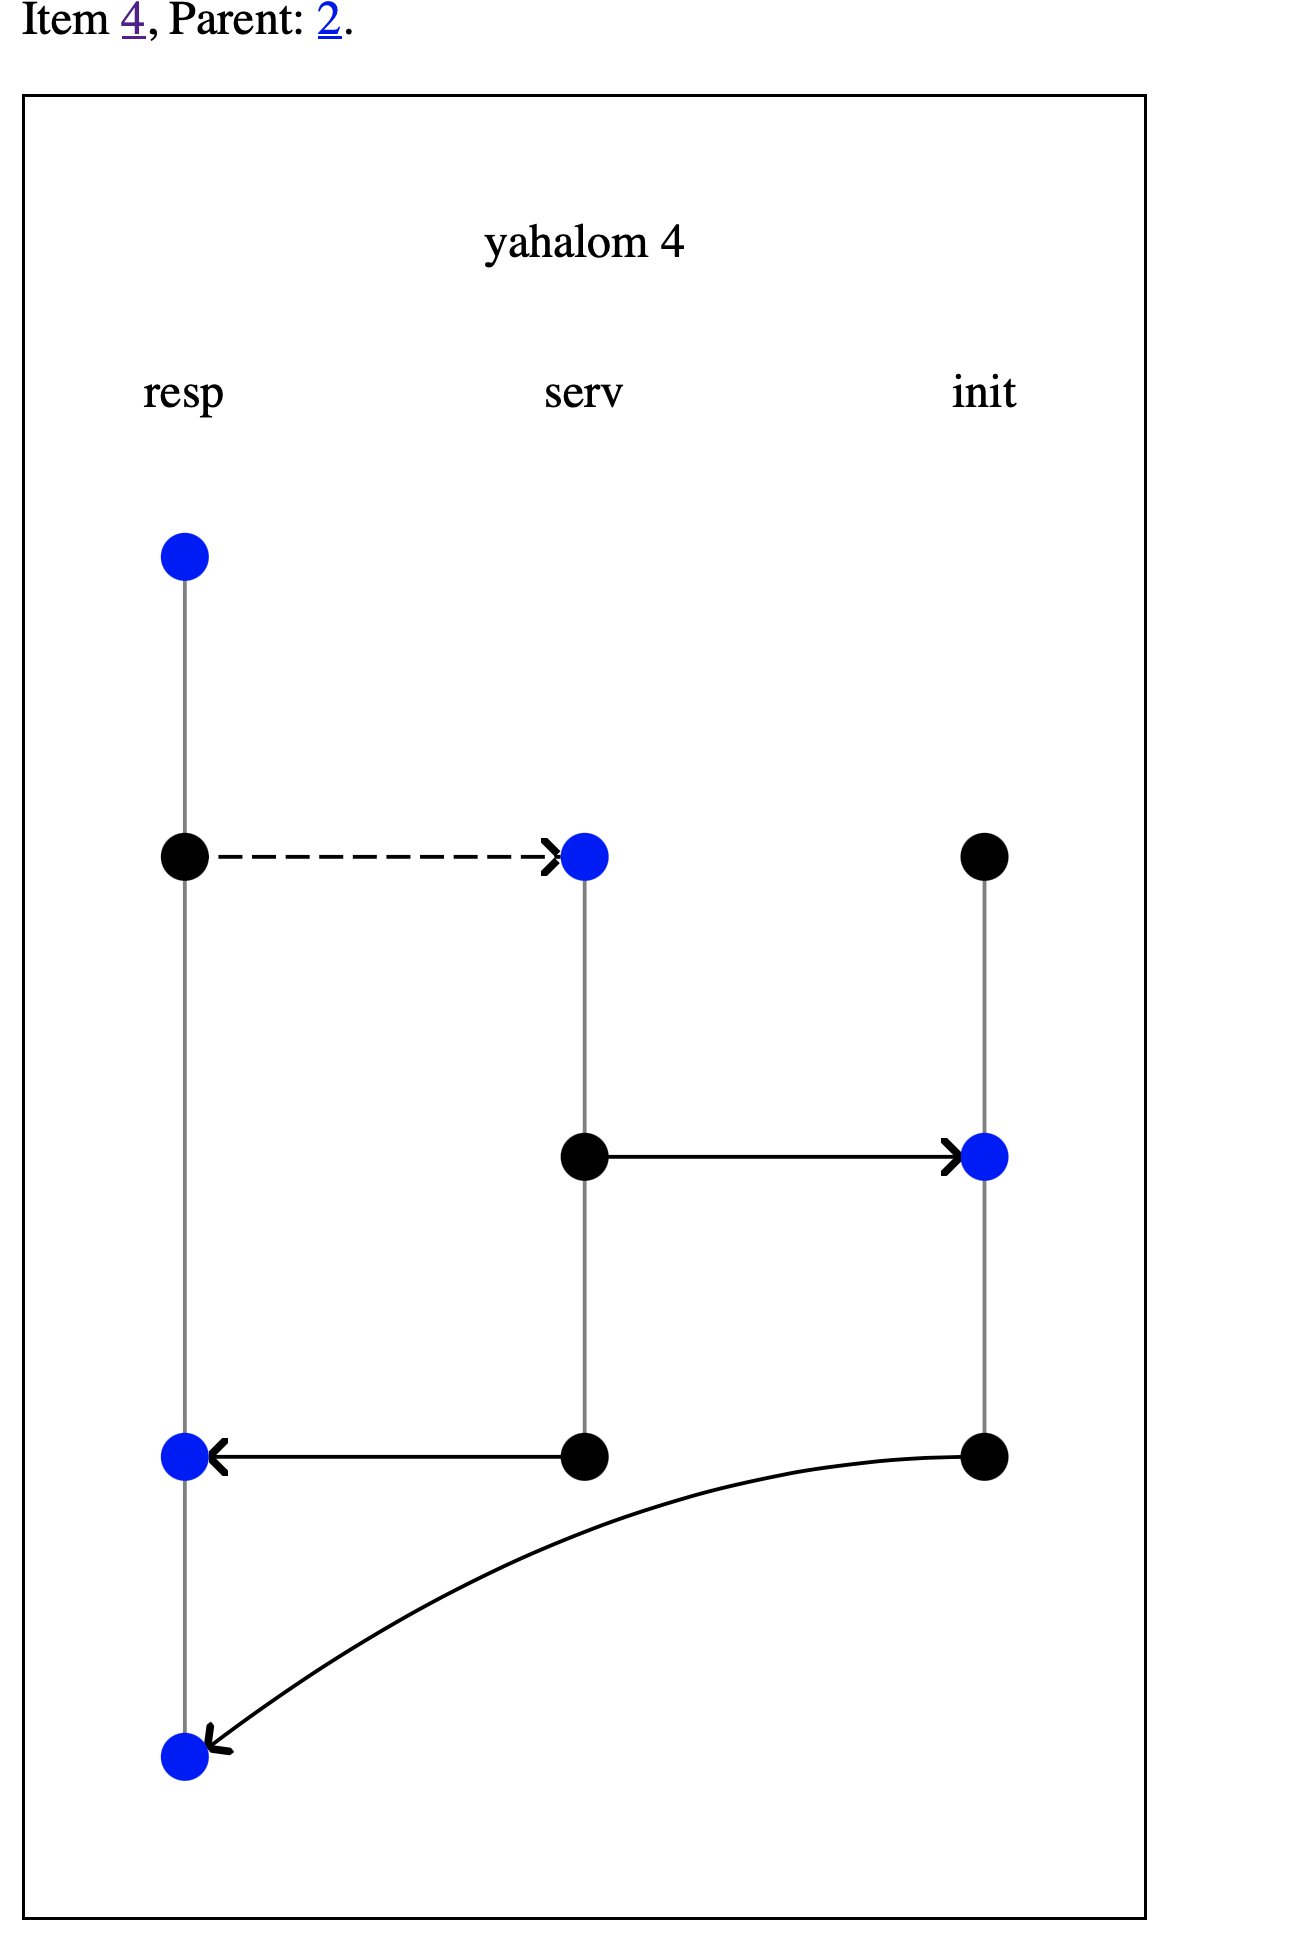
\includegraphics[height=2.5in]{yahalom_ch_resp_pov.png}
  \end{minipage}
  \begin{minipage}[c][2.5in][c]{.5\linewidth}\small
\begin{verbatim}(defstrand resp 4 (k k) (n-a n-a)
           (n-b n-b) (b b) (a a) ...)

(defstrand serv 3 (k k) (n-a n-a-0)
           (n-b n-b) (a a) (b b) ...)

(defstrand init 3 (k k) (n-a n-a-0)
           (n-b n-b) (a a) (b b) ...)
\end{verbatim}
  \end{minipage}
  \caption{The responder's point of view}
  \label{fig:yahalom:ch:resp:pov}
\end{figure}
%
{\cpsa} also validates that the session key $K$ cannot be disclosed.

When we ask what follows if the initiator has a full local session,
the result is more limited.  The initiator authenticates a server
session of at least length two, agreeing on the identities $A,B$, the
two nonces, and the session key $K$.  Again, {\cpsa} validates that
$K$ cannot be disclosed.

Observe that if any initiator and responder have local sessions
involving a shared key $K$, then at least the result of
Fig.~\ref{fig:yahalom:ch:resp:pov} must hold, and they agree on each
other's identities $A,B$.

The server receives no authentication guarantees from the protocol as
defined here, but is guaranteed that the shared key $K$ will remain
undisclosed.  This is undesirable from one point of view, as it may
cost resources for the key server to generate a new key and package
it.  Thus, an adversary can force this to occur as desired.  This is
(presumably) the reason why the original Yahalom protocol encrypts the
message from the responder to the server (the arrow that appears
dashed in Fig.~\ref{fig:yahalom:ch:resp:pov}).  We may achieve the
desired effect by stipulating that the server's channel \verb|ch1| is
authenticated.  Our analysis shows that there is no benefit to
confidentiality on that channel.

One might, however, doubt whether there is much benefit to the
\texttt{(auth ch1)} stipulation, since the adversary can still arrange
for messages from legitimate responders to be delivered repeatedly.

We can infer from this analysis that symmetric authenticated
encryption long term key shared between the key server and each client
is a good way to implement the channels \verb|ch2| and \verb|ch3|,
since the key server relies on their confidentiality property and the
clients rely on their authentication property.

\subsection{Yahalom with Channels, 2:  Per-strand assumptions}
\label{sec:channels:state:ch:strand:level}

We now remove the role definition annotations, i.e.~we omit the
\texttt{(conf ch3 ch2)} annotation from the declaration of the server,
and we omit the \texttt{(auth ch2)} and \texttt{(auth ch3)}
annotations from the responder and initiator declarations, resp.  We
will now ask a succession of queries, each eliciting some more
information, and allowing us to add small assumptions at each stage to
identify the individual channel properties that matter.  First, we
ask:
%
{\small
\begin{verbatim}(defskeleton yahalom
  (vars (a b c name) (n-b text) (ch1 ch2 chan))
  (defstrand resp 4 (a a) (b b) (n-b n-b) (ch1 ch1) (ch2 ch2))
  (auth ch2)
  (uniq-orig n-b))\end{verbatim}}
%
This yields the output in Fig.~\ref{fig:yahalom:q:resp:pov:1}.
%
\begin{figure}
  \begin{minipage}[c][2in][c]{.25\linewidth}
    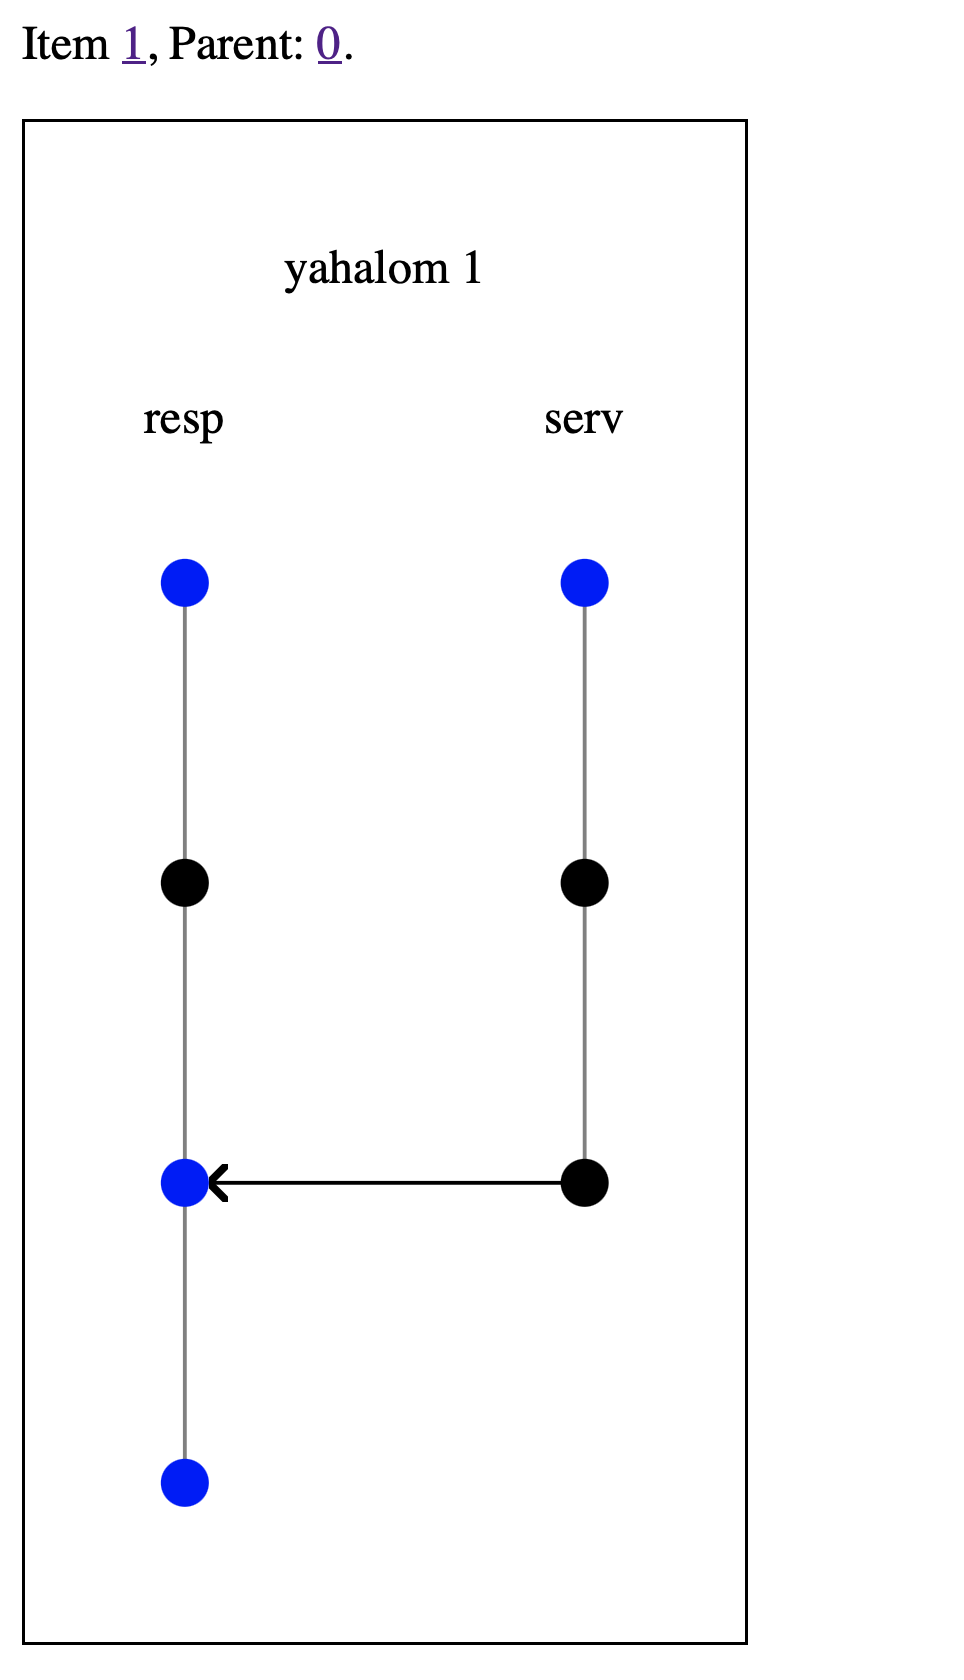
\includegraphics[height=2in]{yahalom_q_resp_pov1.png}
  \end{minipage}
  \begin{minipage}[c][2in][c]{.7\linewidth}\small
\begin{verbatim}(defskeleton yahalom
  (vars (k skey) (n-b n-a n-a-0 n-b-0 text)
                 (a b name) ...)
  (defstrand resp 4 (k k) (n-a n-a) (n-b n-b)
                    (b b) (a a) ...)
  (defstrand serv 3 (k k) (n-a n-a-0) (n-b n-b-0)
                    (a a) (b b) ...)
  (precedes ((1 2) (0 2)))
  (uniq-orig k n-b)
  (auth ch2) ...) \end{verbatim}
  \end{minipage}
  \caption{Responder's first guarantee}
  \label{fig:yahalom:q:resp:pov:1}
\end{figure}

Now that we have ascertained a server run occurred with the same
identities $A,B$ and session key $K$, we may resubmit this output to
{\cpsa} with the added annotation \texttt{(conf ch2 ch3)}, saying that
we will assume that \emph{this} server session successfully used
channels with the confidential property.  At this point, {\cpsa}
completes the analysis with the same shape shown in
Fig.~\ref{fig:yahalom:ch:resp:pov}.

This establishes that no other channel assumptions could be relevant
to the conclusion.  This was not evident from
Fig.~\ref{fig:yahalom:ch:resp:pov}, since other channel assumptions
may have led {\cpsa} to discard some branches of analysis as
impossible, which might then never be displayed.

The analysis from the initiator's point of view can then follow the
same pattern.

\section{State}
\label{sec:channels:state:state}

{\cpsa} models situations in which regular principals control devices
with state registers or storage locations---we will henceforth use the
term \emph{location} for all such pieces of memory---that allow long
term storage and coordination among different local protocol sessions.%
%
\footnote{Allowing the Dolev-Yao adversary to have devices does not
  strengthen its powers, as it can already remember unbounded numbers
  of messages and perform all the reasonable operations on them.  This
  is why our model highlights devices under the control of the regular
  principals.}
%
Each protocol role determines when a regular principal reads from a
device location; what it does with the value read from it, and the
parts of the value; and when it writes a new value into a location.

\paragraph{Locations and channels.}  As we mentioned at the start of
the chapter, {\cpsa} relies on the analogy between reading from
locations and receiving messages from channels, and between writing to
locations and sending messages onto channels.  In particular, writing
to a location is like sending to a confidential channel, as we are
modeling regular principals in control of the devices.  And reading a
state value is partly like receiving from an authenticated channel:
Unless the value read might be the result of device initialization, it
must have been written by a previous write action by a regular
principal.  We say that a value is a \emph{generated state value} when
we model it as not a possible result of device initialization.  When
{\cpsa} knows of a value read from a location that it is a generated
state value, it treats this as an authenticated channel reception.  It
then investigates the possible ways that regular principals may
previously have written this state value to the location.

\paragraph{Contrast:  Locations are mutable.}  Channels can deliver
the same message more than once, and, since redelivery is never ruled
out, effectively always remember their previous contents.  However,
locations are mutable.  After a transition event observes the value in
a location and writes a new (possibly related) value into the
location, subsequent reads are guaranteed to deliver the new value,
not its predecessor.  Although any number of read events may observe
the same value, a transition event ensures that the new value is the
only value available from this location.  This fact---that transitions
erase the past---is the essential characteristic of mutable state.
\index{mutable state}
\index{state}


\paragraph{``Leads to.''}  When a state transition event $n_0$ writes
a value $v$ into a state location $\ell$, and a later observation or
transition event $n_1$ obtains this value $v$ from $\ell$, without any
other transitions having occurred to $\ell$ in between, we say that
$n_0$ \emph{leads to} $n_1$, and we write $n_0\leadsto n_1$.
\index{leads-to relation}


Thus, when $n_0\leadsto n_1$ the following conclusions hold:
\begin{renumerate}
  \item $n_0$ and $n_1$ are events on the same location $\ell$;
  \item  $n_0$ is a transition event;
  \item $n_0$ precedes $n_1$, also written $n_0\prec n_1$; and
  \item $n_1$ receives the value that $n_0$ has written into $\ell$.
\end{renumerate}
%
The event $n_1$ may just be a state observation rather than a state
transition.  In the former case, it is a pure read against $\ell$.  In
the latter case, it is the beginning of a transition event, which we
think of as consisting of a read of the old value in $\ell$ followed
by a write of the new value into $\ell$.

Internally, {\cpsa} represents a state event as transmitting or
receiving a pair $t=(p,v)$.  The second component is the state value
$v$ being read or written.  The first component is a special value
which is thought of as a spacetime point $p$.  If the event is a write
event, then {\cpsa} assumes $p$ to be uniquely originating.  {\cpsa}
defines $n_0\leadsto n_1$ to hold iff (i) $n_0$ is a state node; (ii)
$n_0\prec n_1$, and (iii) for some message $t$, $n_0$ transmits $t$
and $n_1$ receives $t$.

This {\cpsa} representation lets us add to (1)--(4) another
conclusion:  When $n_0\leadsto n_1$,
%
\begin{renumerate}
  \item if also $n_2\leadsto n_1$, then $n_0=n_2$.
\end{renumerate}

\subsection{The axioms of state}
\label{sec:channels:state:axioms}

The mutating, past-erasing property of transitions is expressed in two
basic properties of the leads-to relation.  They say in essence that
leads-to is \emph{discrete} for transitions events on any one
location.

We write them diagrammatically in Fig.~\ref{fig:leads:to}, using a
boxed variable $\xymatrix@1{*+[F]{\,m\,\strut}}$ to represent a
transition event, and a plain variable $m$ to represent an event that
may be either a transition or a pure observation.  We use a wavy arrow
to represent leads-to; a dotted arrow to represent the precedence
ordering $\prec$; and $\preceq$ to express the weak ordering,
i.e.~$n_0\preceq n_1$ holds if and only if $n_0\prec n_1$ or
$n_0=n_1$.
%
\begin{figure}
  \centering
  %
  \[(i)\qquad
    \xymatrix@R=1mm@C=4mm{&
      *+[F]{n}\ar@{~>}[ddl]\ar@{.>}[ddr]^{\prec} & & & &
      *+[F]{n}\ar@{~>}[ddl]\ar@{.>}[ddr]^{\prec} \\
      & & & \Longrightarrow &    \\
      *+[F]{m_0} & & *+[F]{m_1} & &
      *+[F]{m_0} & \textcolor{red}{\preceq} & *+[F]{m_1} }
    %
  \]\vspace{3ex}
  %
  \[(ii)\qquad
    \xymatrix@R=1mm@C=4mm{*+[F]{m_0}\ar@{.>}[ddr]_{\prec} & &
      *+[F]{m_1}\ar@{~>}[ddl] & &
      *+[F]{m_0}\ar@{.>}[ddr]_{\prec} &\textcolor{red}{\preceq} &
      *+[F]{m_1}\ar@{~>}[ddl]\\
      & & & \Longrightarrow   \\
      & n && && n}
  \] 
  \caption[Leads-to axioms]{Two axioms about state events on the same
    location $\ell$}
  \label{fig:leads:to}
\end{figure}
%
\index{mutable state!axioms}

In each case, the events $n,m_0,m_1$ are all state events on the same
location $\ell$.
%
\begin{description}
  \item[Axiom (i)] states that when $n\leadsto m_0$ and $n\prec m_1$,
  all of these being transition events on $\ell$, then
  $m_0\preceq m_1$.  Thus, the leads-to relation is a discrete step,
  and if $m_0\not= m_1$, then the latter comes definitely later.

  We call axiom (i) the \textbf{discrete-after} axiom, since it forces
  $m_1$ to come after a transition that is the target of the
  $\leadsto$ edge.
  \item[Axiom (ii)] states that when $m_0\prec n$ and $m_1\leadsto n$,
  each $m_i$ being a transition on $\ell$, then $m_0\preceq m_1$.
  Again, the leads-to relation is a discrete step, and if
  $m_0\not= m_1$, then the former comes definitely earlier.

  We call axiom (ii) the \textbf{discrete-before} axiom, since it
  forces $m_0$ to come before a transition that is the source of the
  $\leadsto$ edge.
\end{description}
%
The symmetry between these two principles is better brought out if we
omit to state, in (i), that $n$ is a transition.  The source of a
leads-to edge is always a transition.  The common idea is that a weak
ordering holds between $m_0$ and $m_1$, whenever one is a connected to
$n$ by $\leadsto$ and the other by $\prec$.  They jointly say:  a
transition ordered with respect to one end of a leads-to arrow has the
corresponding weak ordering with respect to the other end.

%   Their concrete form may be found in the output of {\cpsa}
%   specifications using state, such as~\texttt{examples/open-closed.tst},
%   although {\cpsa} refers to them as the \texttt{shearsRule} and
%   \texttt{invShearsRule}, resp.

\subsection{Consequences of the axioms}
\label{sec:channels:state:consequences}

What is distinctive of state---over and above channel confidentiality
and channel authenticity for generated state values---is captured in
the \emph{discrete-after} and \emph{discrete-before} axioms.  However,
each of them has a disjunction as its conclusion, namely either
$m_0=m_1$ or $m_0\prec m_1$.  Disjunctions are logically less
convenient than non-disjunctive conclusions, since separate
possibilities must each be explored.
%
\begin{figure}
  \centering\[ \xymatrix@R=1mm@C=1mm{&
      *+[F]{n}\ar@{~>}[ddl]\ar@{~>}[ddr] & \\
      & & & \Longrightarrow &  \textcolor{red}{m_0=m_1}  \\
      *+[F]{m_0} & & *+[F]{m_1}} \qquad\qquad
    %
    \xymatrix@R=1mm@C=1mm{&
      *+[F]{n_0}\ar@{~>}[ddl]\ar@{.>}[ddr]^{\prec} & \\
      & & & \Longrightarrow &  \textcolor{red}{\mathsf{false}}  \\
      *+[F]{n_1} &\succ & *+[F]{m}}
    %
  \]
  \[ \xymatrix@R=1mm@C=4mm{&
      *+[F]{n_0}\ar@{~>}[ddl]\ar@{~>}[ddr] & \\
      & & & \Longrightarrow &  \textcolor{red}{\mathsf{false}}  \\
      *+[F]{n_1} &\prec & {m}}
    %
  \]
  \caption{Three derived rules for state:  Scissors, no interruption,
    and cake}
  \label{fig:derived:state:rules}
\end{figure}
%
Hence, {\cpsa} also formalizes three consequences of the discreteness
axioms.  One of them has the conclusion $m_0=m_1$, and the other two
have the conclusion \emph {false}.  Again assuming that the state
events concern the same location $\ell$, the rules are:
%
\begin{description}
  \item[Scissors rule,] which says that when a given node $n$ leads to
  transition nodes $m_0,m_1$, the latter two are equal.

  Equivalently, a single node leads to at most one transition node.
  \item[No interruption,] which says that a transition node $m$ is
  never properly between transition nodes $n_0$ and $n_1$ when
  $n_0\leadsto n_1$.

  Thus, a transition node $m$ cannot ``interrupt'' the leads-to edge.
  \item[Cake rule,] which says that if a node $n_0$ leads to two other
  nodes, and one of them is a transition $n_1$, then the other one $m$
  does not follow the transition.

  Thus, it says that a transition $n_1$ caps off the period when other
  events $m$ (which are pure observations by the scissors rule) may
  result from $n_0$.
\end{description}
%
We present these diagrammatically in
Fig.~\ref{fig:derived:state:rules}.  The two leads-to edges of the
\emph{scissors rule} are like the blades, which the equation
${m_0=m_1}$ snaps shut.  The cake rule formalizes the fact that you
can't eat your cake at $n_1$ and have it too at $m$, at least not if
$m$ follows $n_1$.

Again, their concrete form may be found in the output of {\cpsa}
specifications using state, such as~\texttt{examples/open-closed.tst}.

\paragraph{Why these rules are consequences.}  Each of these rules is
easily justified from the discrete-after and discrete-before rules,
using the facts that $n\leadsto m$ implies $n\prec m$ and that
$\preceq$ is a (weak) partial order.

\begin{description}
  \item[Scissors rule:]  The scissors rule follows by two applications
  of the discrete-after axiom.  Specifically, since $n\leadsto m_1$
  implies $n\prec m_1$, we can apply the discrete-after axiom to infer
  that $m_0\preceq m_1$.  Symmetrically, observing thay
  $n\leadsto m_0$ implies $n\prec m_0$, we can again apply the
  discrete-after axiom to infer that $m_1\preceq m_0$.

  The antisymmetry of $\preceq$ implies that $m_0=m_1$.
  \item[No interruptions rule:]  For the no interruptions rule, apply
  discrete-after to infer that $n_1\preceq m$.  But since
  $m \prec n_1$ is also assumed, this would yield a cycle.
  \item[Cake rule:]  For the cake rule, apply discrete-before,
  instantiating its variable $m_0$ as $m$, its $m_1$ as $n_0$, and its
  $n$ as $n_1$.  Thus, it follows that $m\preceq n_0$, but the
  leads-to edge $n_0\leadsto m$ implies $n_0\prec m$, yielding a
  contradiction.
\end{description}

\subsection{Syntax for state}
\label{sec:channels:state:syntax}

In defining the syntax for modeling state, we first describe state
events and the state segments that they can build up.  We then
describe how to specify generated state values---which were mentioned
at the beginning of the chapter---and critical sections---which are
atomicity assumptions about state segments.

\paragraph{State events and state segments.}  In addition to the
\verb|chan| sort discussed in Section~\ref{sec:channels:state:ch},
there is a sort \verb|locn|.  A variable \verb|lv| declared of sort
\verb|locn| via a declaration such as \verb|(lv locn)| may be used as
the target of \verb|load| and \verb|stor| events; these events
indicate that a value is to be read from a location or written to it.
Thus, Fig.~\ref{fig:dev:open}, which uses a number of operators from a
\texttt{lang} field,%
\footnote{See Section~\ref{sec:algebra:lang:field}.  In this example,
  \texttt{dev-key-state}, \texttt{open-req}, \texttt{door-state}, and
  \texttt{opened} are tuple operators, and \texttt{hash-dk} is a hash
  operator, in essence a key derivation function.  This example is
  found in~\texttt{examples/open-closed.scm}.}
%
shows a role that manipulates two variables \texttt{lk, ls} of sort
\verb|locn|.  Its intent is to open a door in response to a suitable
encrypted command, conforming its action.
%
\ttindex{locn} 
%
\begin{figure}\small
  %
\begin{verbatim}(defrole dev-open
    (vars (k skey) (n nb text) (any mesg) (d o b name) (lk ls locn))
    (trace
     (load lk (dev-key-state d o k))
     (recv (cat b n (enc (open-req b d o nb n) (hash-dk (cat b nb n k)))))
     (load ls (door-state d any))
     (load lk (dev-key-state d o k))         ; check k unchanged
     (stor ls (door-state d (opened b nb n)))
     (send (hash (open-req b d o nb n))))
    (gen-st (dev-key-state d o k))
    (facts (same-dev ls lk)))\end{verbatim}
  %
  \caption{Device-open role causing door to open}
  \label{fig:dev:open}
\end{figure}
%
The form \texttt{(lk ls locn)} declares the variables of sort
\verb|locn|.  The form \texttt{(load lk (dev-key-state d o k))} loads
a tuple including a key \verb|k| from the \verb|locn| \verb|lk|, which
must contain a tuple of this kind for the event to occur.  After
receiving a message that contains a request to open the door, it loads
the current door state from the other location \verb|ls|, after which
it stores back the ``open'' value.  These events might be implemented
by a sensor and an actuator in a real device.  Finally, it confirms
success by sending the hash of the open request.

A \verb|load| or \verb|stor| event always contains a location variable
followed by a message term, just like a channel \verb|send| or
\verb|recv| (Section~\ref{sec:channels:state:ch}).
\ttindex{load}
\ttindex{stor}


Observe that the \verb|stor| event immediately follows a \verb|load|
event, and this is in fact always the case.  Since together they
represent a transition that consumes an old value that will no longer
be available after the the transition, the \verb|stor| event always
follows a paired \verb|load| event.  Together, they form a \emph{state
  segment}.  However, state segments may be longer than a single pair
of events.

In general, a state segment consists of one or more \verb|load|
events followed by zero or more \verb|stor| events, subject to the
requirements that:
%
\begin{enumerate}
  \item no two \verb|load| events in this state segment load from the
  same location;
  \item no two \verb|stor| events in this state segment store into the
  same location;
  \item each \verb|stor| event stores into a location from which a
  value was \verb|load|ed in this state segment.
\end{enumerate}
%
A particular state segment is a \emph{transition for} a location
$\ell$ iff there is a \verb|stor| into $\ell$ in this state segment.
It is a \emph{(pure) observation for} $\ell$ iff there is a
\verb|load| from $\ell$ but no \verb|stor| into $\ell$ in this state
segment.

We use state segments of length greater than two to represent events
that involve multiple locations.  If a transition for location
$\ell_1$ depends on the value present in $\ell_2$, then a state
segment can load $v_1$ and $v_2$ from $\ell_1$ and $\ell_2$
(resp.)~and then store a new value dependent on $v_1,v_2$ into
$\ell_1$.  In this case, the state segment is a transition for
$\ell_1$ but a pure observation for $\ell_2$.  If instead new values
are stored into both $\ell_1$ and $\ell_2$, then the state segment is
a transition for both.  In other cases, a state segment loads from
both $\ell_1$ and $\ell_2$, but instead of storing back to either of
them, it simply uses those values to control future message
transmissions and receptions.  In the latter cases, the state segment
is a pure observation for both $\ell_1$ and $\ell_2$.

\paragraph{Rules for protocols with
  state.}  \label{state:gen:rules:start} {\cpsa} generates three types
of rules for protocols that manipulate state, in addition to the two
axioms of Section~\ref{sec:channels:state:axioms} and the three
consequences of Section~\ref{sec:channels:state:consequences}.%
%
\footnote{See Section~\ref{sec: rules} for rules in {\cpsa}.}

The first kind are the \emph{transition rules}, and these are
generated entirely automatically by {\cpsa}.  The axioms and rules of
Sections~\ref{sec:channels:state:axioms}--\ref{sec:channels:state:consequences}
depend on which events are transition events, the boxed events in
Figs~\ref{fig:leads:to}--\ref{fig:derived:state:rules}.  Moreover, the
syntax of the state segments determines which these are.  Thus,
{\cpsa} generates rules that imply that an event is a transition event
if:
%
\begin{enumerate}
  \item it is a \verb|stor| event; or
  \item it is a \verb|load| event, and the strand is long enough also
  to have a \verb|stor| event from this state segment for the same
  location $\ell$.
\end{enumerate}
%
These are the transition rules.
\ttindex{trans}

The second kind are the \emph{generated state value rules}.  As we
mentioned at the start, a generated state value is a value $v$ that is
definitely non-initial.  Thus, if a \verb|load| event reads a
generated state value $v$ from a location $\ell$, then $\ell$ is
acting like an authenticated channel for $v$.  In particular {\cpsa}
will consider which instances of the roles could previously have
stored $v$ into $\ell$; one of those must be present.
\index{generated state value}

A generated state assumption may be introduced as a per-strand
assumption, akin to the declarations discussed in
Section~\ref{sec:channels:state:ch:strand:level}.  In that case it is
syntactically present in a {\cpsa} \texttt{defskeleton} query such as:
%
{\small
\begin{verbatim}(defskeleton open-closed
  (vars (k skey) (d o name))
  (defstrand dev-pass 4 (k k) (d d) (o o))
  (gen-st (dev-key-state d o k)))
\end{verbatim}}
%
This \texttt{gen-st} declaration says that the particular tuple
\texttt{(dev-key-state d o k)} using the values of the variables that
appear in this strand forms a generated state value.
\ttindex{gen-st}


A generated state assumption may be introduced as a role-level
assumption, akin to the declarations discussed in
Section~\ref{sec:channels:state:ch:role:level}.  In this case, the
specifier wants to tell {\cpsa} that the declared value is a generated
state value whenever an instance of the role is long enough to furnish
values for the variables that appear in it.  Fig.~\ref{fig:dev:open}
contains a role-level generated state assumption, namely
\texttt{(dev-key-state d o k)}.  Since the trace of the
\texttt{dev-open} rule loads a value of this form as its first action,
these variables have values in every instance of height $\ge 1$.

{\cpsa} enforces this role-level assumption by generating a rule
stating:
%
{\small
\begin{verbatim}(defgenrule gen-st-dev-open-0
    (forall ((z strd) (k skey) (o d name))
      (implies
        (and (p "dev-open" z 1) (p "dev-open" "k" z k)
             (p "dev-open" "o" z o) (p "dev-open" "d" z d))
        (gen-st (dev-key-state d o k)))))
\end{verbatim}
}
%
\noindent{\cpsa} uses the \texttt{defgenrule} form to distinguish
rules it has generated automatically from rules that were explicitly
written by the specifier, as described in Section~\ref{sec: rules}.

Finally, the third kind of rule concerns \emph{critical sections}.
%
\begin{figure}\small
%
\begin{verbatim}(defrole dev-up
    (vars (k skey) (d o name) (old old1 mesg) (ch chan) (lk ls locn))
    (trace
     (recv ch (cat "power-up" d o k))
     (load lk old)
     (load ls old1)
     (stor lk (dev-key-state d o k))
     (stor ls (door-state d (closed o)))
     (send (enc "up" k)))
    (auth ch)
    (critical-sections (1 4))
    (facts (same-dev ls lk)))
\end{verbatim}
%
  \caption{Critical section declaration}
  \label{fig:critical:section}
\end{figure}
%
%
\begin{figure}\small
  %
\begin{verbatim}  (defgenrule cau-dev-up-2
    (forall ((z z1 strd) (i indx))
      (implies
        (and (p "dev-up" z 3) (prec z1 i z 2))
        (or (= z z1) (prec z1 i z 1)))))

  (defgenrule eff-dev-up-3
    (forall ((z z1 strd) (i indx))
      (implies
        (and (p "dev-up" z 4) (prec z 3 z1 i))
        (or (= z z1) (and (p "dev-up" z 5) (prec z 4 z1 i))))))\end{verbatim}
%
  \caption{Critical section:  Generated rules}
  \label{fig:critical:section:rules}
\end{figure}
%
A critical section declaration in the definition of a role takes the
form \texttt{(critical-sections (i j))}, where the trace must have a
state segment that starts at or before event \emph{i} and ends at or
after event $j$, where these are 0-based indices.  It implies that any
node that precedes one of the load events must precede all of them.
Any node that follows one of the store events must follow all of them.
Thus for instance in Fig.~\ref{fig:critical:section}, the load events
at indices 1, 2 and the store events at indices 3, 4 occur with
transaction-like atomicity.  This declaration would cause {\cpsa} to
generate the rules in Fig.~\ref{fig:critical:section:rules}.  They are
of value only when the state segment has multiple loads or multiple
stores.  In this particular example, the critical section declaration
does not in fact make a difference to the analysis. 
%
\label{state:gen:rules:end}

\subsection{Channels and state:  Summary}
\label{sec:channels:state:summary}

A core idea is that receptions may have \emph{authenticity}, meaning
that the adversary has not delivered the message; thus, {\cpsa}
explores what regular strands may have transmitted it.  Dually, a
transmission may have \emph{confidentiality}, meaning that the
adversary will not receive the message directly.  Thus, any parts of
the transmitted message that appear in new forms subsequently will
require some regular strand to have received it and transformed these
parts.

In the {channel} mechanism, {\cpsa} allows these properties to be
directly associated with channels, providing a useful technique for
protocol design.  In the state mechanism, {\cpsa} models the
\emph{confidentiality} of storing a value into a device controlled
locally by the regular principal(s).  Moreover, \emph{stored} state
values with the \texttt{gen-st} property satisfy the
\emph{authenticity} condition also.

Besides these properties, mutable state also requires modeling the
fact that an old state value can no longer be observed in a location
after that location has undergone a transition.  We express these in
the two axioms of Fig.~\ref{fig:leads:to}; {\cpsa} also uses their
three consequences as shown in Fig.~\ref{fig:derived:state:rules} for
efficiency.

The modeling distinguishes between \emph{transitions} on a location,
which are expressed in state segments that contain a \verb|stor| to
it, and \emph{observations}, expressed in state segments that contain
a \verb|load| but no \verb|stor| to it.  {\cpsa} determines which
events are transitions on a location automatically, and generates
rules to keep track of this information.  Rules are also available to
determine which state values are \emph{stored} state values, and these
are generated from \texttt{gen-st} declarations.

{\cpsa}'s job is to enumerate shapes.  When a specification
distinguishes a kind of value that can only appear in an initial
\verb|load|, and transitions that do not produce these values, but
always produce \emph{stored} state values with the \texttt{gen-st}
property, then a run can typically have 0, 1, 2, \dots, $n$
transitions, and these will have no homomorphisms between them.  Hence
there will be infinitely many distinct shapes to enumerate, and
{\cpsa} will not terminate, although its partial outputs are often
informative.  The craft of using {\cpsa} to understand state in
protocols is often to restrict the \texttt{gen-st} declarations so
that {\cpsa} does not distinguish among state histories of
(irrelevantly) different lengths.

%%% Local Variables:
%%% mode: latex
%%% TeX-master: "cpsa4manual"
%%% End:

%
\chapter{Trace constraints}
\label{chap:trace:constraints}

In some cases, one wants to declare properties that all of the
``real'' instances of a role must satisfy.  For instance, possibly two
parameters will never receive the same value, e.g.~because a server is
required to check that the client name in a transaction is different
from its own name.  {\cpsa} presents several ways of ensuring such
constraints, some of which may be logically indistinguishable as far
as {\cpsa} is concerned, while representing different operational
consequences for other tools, such as the Zappa {\cpsa}-to-Rust
compiler.

%%  Must include:  rely; guarantee; cheq  



%%% Local Variables:
%%% mode: latex
%%% TeX-master: "cpsa4manual"
%%% End:


\part{Reference material}
\label{part:reference}
\chapter {Troubleshooting}
\label{ch:troubleshooting}

The {\cpsa} tool is a complicated one and many errors are possible in
its use.  In this chapter we discuss these errors, from the simplest
to the most complex, and offer suggestions as to how to resolve them.

\section{Non-termination}
\label{sec:bounds}

The {\cpsa} tool is not guaranteed to complete its search on all
well-formed inputs.  The problem space {\cpsa} attempts to perform
includes some Turing-undecidable problems.

Because of this, the tool has two bail-out conditions that users should be
aware of:

\begin{itemize}

\index{strand bound}
\item The {\bf strand bound} causes the tool to abort its analysis if any
skeleton it analyzes has more strands than the bound.  By default, the strand
bound is 12.

\index{step limit}
\item The {\bf step limit} causes the tool to abort its analysis if during
the analysis of a single input \texttt{defskeleton} or \texttt{defgoal}, the
number of skeletons it processes exceeds the limit.  By default, the step limit
is 2000.

\index{depth limit}
\item The {\bf depth limit} causes the tool to not analyze skeletons
  more steps away from the initial point of view than the bound.
  There is no depth limit by default.  Skeletons that are unrealized and not
  analyzed due to the depth limit are marked with ``\texttt{(fringe)}''.

\end{itemize}

If you execute an analysis and the tool says ``Strand bound exceeded''
or ``Step limit reached,'' then that bail-out condition has come into play.
This may indicate an analysis that would never terminate, but it may also be
the case that the strand bound or step limit is too small, and a larger one will
enable the analysis to complete.

Unlike the strand bound and the step limit, the depth limit never
triggers an error condition, and can thus be useful for multi-skeleton
analyses in which one of the earlier skeletons would otherwise have a
non-terminating analysis.

The step limit, depth limit, and strand bound can be adjusted through the
\texttt{limit}, \texttt{depth}, and \texttt{bound} options, respectively.  See
Section~\ref{sec:options}.

\index{interrupting}
Note that sometimes, a user may become impatient waiting for an
analysis to either complete or bail out.  When this happens, the user should
not hesitate to interrupt the tool; the tool will output a partial result that can
be graphed so the user can examing the analysis done so far.

An analysis that doesn't terminate does not necessarily represent an
insecure protocol, it may just indicate a protocol where a more clever
analysis is required than {\cpsa}'s automated one.

\subsection{Tweaking the search}
There are cases in which the default {\cpsa} analysis does not
terminate, but a non-default analysis would terminate.  The tool has
several settings that influence the search but can be tweaked:

\begin{itemize}
\index{try-old-strands option}
\index{reverse-nodes option}
\index{options!try-old-strands}
\index{options!reverse-nodes}
\item {\bf Node precedence.}  In a skeleton with multiple unrealized
  receptions, the tool will, by default, focus on the topmost
  unrealized node of the rightmost strand that contains an unrealized
  node.  If you find that an analysis gets into a large search space
  due to exploring those unrealized receptions first, you could alter
  this order with the \texttt{reverse-nodes} or
  \texttt{try-old-strands} options.  The latter will prioritize the
  leftmost strands over the rightmost, while the former will
  prioritize the bottom-most unrealized node in the strand rather than
  the topmost.

\index{check-nonces option}
\index{options!check-nonces}
\item {\bf Critical term precedence.}  Occasionally, a reception will
  arise that is unrealized and multiple critical terms are available.
  In particular, there are cases where a term contains both a
  hard-to-explain encryption and a restricted nonce.  For instance, in
  the Kerberos protocol, the ticket $\enc{k,a,b}{SK(b,s)}$ can serve
  as both a critical encryption (because $SK(b,s)$ may be declared
  non-originating) and a critical term (because $k$ is uniquely
  originating).  By default, {\cpsa} will treat the encryption as the
  critical term because this tends to lead to learning more in fewer
  steps, but this choice can be reversed by using the
  \texttt{check-nonces} option.

\index{priority}
\item {\bf Priority.}  The tool contains an ability to declare a
  priority for certain receptions that differs from the default.
  Priority takes precedence over all other search orderings.  See
  Section~\ref{sec:decl_syntax} for the format requirements for
  declaring priorities, and the \texttt{priority\_test.scm} example in the
  examples directory.

  Note that the default priority is 5, and priority 0 indicates that
  the tool should never bother solving tests at those nodes.  This may
  be of use, for instance, if solving one particular node leads to
  infinite analysis, but other nodes would result in a quick
  determination that a skeleton is dead.
\end{itemize}

\section{Error messages}
\label{sec:errors}

In this section, we provide an alphabetical listing of error messages
/ failures that may arise during {\cpsa} execution.  If you get an error
message not included here, it likely represents a bug and should be reported
to the tool maintainers.

\begin{itemize}
\item \textbf{``[ASSERT FAILED] [...]''}.  This kind of error should
  not occur.  If you see this happen, please contact the tool maintainers
  and make a bug report!

\item \textbf{``Aborting after applying 500 rules and more are
  applicable''}.  This most likely indicates a circular use of rules.

\item \textbf{``Algebra.absenceSubst: bad absence assertion''} or
  \textbf{``Algebra.nullifyOne: unexpected pattern''} The
  \texttt{absent} declaration must be declared on a pair where the
  first element is an \scap{rndx} variable and the second element is 
  an exponent.
  % or a \scap{base} term.
  %
  These errors should not occur if you did not give {\cpsa} an input
  with an absent declaration.

\item \textbf{``Algebra.inv: Cannot invert a variable of sort mesg''}.
  Variables of the \texttt{mesg} sort should never be used as the key
  in an encryption.  {\cpsa} uses a single function symbol to represent
  both symmetric and asymmetric encryption, and when the key is a variable
  of sort \texttt{mesg}, it is ambiguous which is meant.  As a result,
  it is unclear what the decryption key would be for such a message.  When
  {\cpsa} tries to calculate the decryption key when the encryption key
  is a variable of sort \texttt{mesg}, this error is produced.

\item \textbf{``Atom not unique at node''}.  This occurs when a
  formula has been specified including a \texttt{uniq-at} predicate in
  the antecedent that is untrue.

\item \textbf{``Bad char [...]''}.  This error message comes from a
  low-level parser trying to understand S-expressions.  When parsing
  an S-expression, any non-whitespace that isn't a parenthesis is an
  ``atom'' but we expect atoms to be symbols, numbers, or quoted
  strings, and only certain characters are allowed in these.  An atom
  that starts with a digit is expected to be a number, for instance, so
  subsequent non-digits will cause an error of this kind.  The characters
  allowed in symbols include all alphanumeric characters and the following
  punctuation marks: \verb|+, -, *, /, <, =, >, !, ?, :, $,|  \verb|%, _, &, ~, ^|.

\item \textbf{``Bad height'' / ``Bad position in role'' / ``Negative
  position in role''}.  A \texttt{defstrand} includes a specification
  of a height (the length of the instance) but that height must be
  positive and must not exceed the length of the role.

\item \textbf{``Bad str-prec''}.  Your goal included a
  \texttt{str-prec} predicate among node variables associated with
  different roles.  In other words, your formula has attempted to make
  a single strand that includes events from distinct roles.

\item \textbf{``Close of unopened list''}.  Your input has an erroneous
  close-paren.

\item \textbf{``Disallowed bare exponent''}.  See Section~\ref{sec:dh}.
  The tool requires that within roles and skeletons, exponents occur only
  inside an exponentiation function.

\item \textbf{``Domain does not match range''}.  This error message
  occurs when {\cpsa} is trying to understand the variable assignment
  you have specified in a \texttt{defstrand}.  You may have defined
  the value of a parameter more than once, or your definition may have
  a type mismatch.  For instance if $a$ is a parameter role expected
  to be of the name type, and you declare $t$ to be a text variable,
  then including \texttt{(a t)} in a defstrand will produce this
  error.

\item \textbf{``Duplicate role [...] in protocol [...]''}.  Fairly
  self-explanatory: the roles in a protocol must have distinct names.
  This error occurs if you have two protocols with the same name.

\item \textbf{``Duplicate variable declaration for [...]''}.  Fairly
  self-explanatory: within any \texttt{vars} statement, any symbol may
  be used for a variable name, but each variable name can be declared only once.

\item \textbf{``End of input in string''}.  You included a quote-delimited
  string but didn't close it before the end of the input file.

\item \textbf{``Equals not allowed in antecedent''}.  The \texttt{equals}
  predicate may only be used on the conclusion side of a \texttt{defgoal}.

\item \textbf{``Expansion limit exceeded''}.  This most likely indicates
  a circular use of macros.  The limit of expansion of a macro within a macro is
  hard-coded in the tool as depth 1000.

\item \textbf{``Expecting [...] to be [a/an ...]''}.  You have a type
  error in your use of a function symbol.  For instance if
  \texttt{(pubk a)} is to be loaded within a particular variable
  declaration scope, the $a$ variable should be of the $\scap{name}$
  sort.

\item \textbf{``Expecting a node variable'' / ``Expecting an algebra
  term''}.  Certain predicates within a \texttt{defgoal} expect one of
  their inputs to be a declared node variable (or to be a non-node
  variable).  If a variable used in such an input is declared
  otherwise, this error message is produced.

\item \textbf{``Expecting an atom''}.  Certain declarations, in particular
  the \texttt{uniq-orig}, \texttt{uniq-gen}, and \texttt{non-orig} ones,
  are expected to be used on atomic terms rather than compound ones.

\item \textbf{``Expecting terms in algebra [...]''}.  The tool
  actually expects to know the message algebra to use up front, before
  it begins parsing.  The algebra is the basic one by default, or you
  may specify through a command-line argument or a herald to use the
  Diffie-Hellman algebra.  Each \texttt{defprotocol} in the input
  specifies an algebra to use, and this error occurs when that algebra
  doesn't match the one {\cpsa} is prepared to parse.  To resolve:
  check that you aren't requesting the wrong algebra, and check that
  you have properly spelled the name of the algebra in your
  \texttt{defprotocol}.

\item \textbf{``Identifier [...] unknown''}.  This is a relatively common
  user-caused error that occurs when you try to use a variable not declared
  in your \texttt{vars} declaration.

\item \textbf{``Include depth exceeded with file [...]''}.  Most
  likely, this indicates a circular use of the \texttt{include}
  command.  The limit of inclusion within an included file is depth
  16.

\item \textbf{``Keyword [...] unknown''}.  The tool was expecting the symbol
  to specify an algebra function symbol, but it didn't match any of the available
  ones.  This most commonly indicates that the user forgot to include a
  function symbol name at the beginning of a list when describing a term.  One of
  the most common forms of this mistake is to include \texttt{(send (a b))} in
  a trace of a role, when the user intended to model the sending of the pair $(a,b)$.
  The proper input would be \texttt{(send (cat a b))}.

  Because of this type of mistake, it is recommended to avoid using variables
  in your model that are the same as function symbol names such as
  ``ltk'' or ``pubk''.

\item \textbf{``In a rule equality check, cannot find a binding for
  some variable''}.  An equality in a rule is receiving a variable
  that has not been bound by a length or parameter predicate.  Try
  moving the equality to the end of the conjunction in which it
  occurs.

\item \textbf{``In rule [...], parameter predicate for [...] did not
  get a strand''}.  This message occurs when a strand variable is not
  bound by a length predicate.

\item \textbf{``In rule [...], [...] did not get a strand''}.
  This message occurs when a strand variable is not bound by a length
  predicate.

\item \textbf{``In rule [...], [...] did not get a term}.  This
  message occurs when an algebra variable is not bound by a parameter
  predicate.

\item \textbf{``Malformed [...]''}.  Generally speaking, this indicates
  a syntax error.  Consult the grammar in Chapter~\ref{ch:input} for the
  syntax requirements for the type of object the tool claims was malformed.
  Double-check that you have spelled required keywords correctly, and that
  your parentheses are matched.

\item \textbf{``Malformed association list''}.  This refers to one of
  the ``-alist'' symbols in the grammar; these may occur in skeletons,
  goals, protocols, or roles.

  Association lists are lists of S-expressions, each of which is a
  list that starts with a symbol.  This error would occur if you had,
  for instance, a symbol or a number, or an S-expression starting with
  a number as an input to a \texttt{defrole} or \texttt{defskeleton}.

\item \textbf{``Malformed input''}.  Top level S-expressions in your
  input file must be one of the following: \texttt{defprotocol,
    defskeleton, defgoal, comment,} or \texttt{herald}.  The tool also
  recognizes \texttt{defpreskeleton} as a synonym for
  \texttt{defskeleton}.  If you have an S-expression at the top level
  that is other than one of these, this is the error message you will
  see.

\item \textbf{``Malformed pair -- nodes in same strand''}.  In a \texttt{defskeleton}
  you are prohibited from specifying orderings between nodes in the same strand.

  This is not the case for \texttt{leadsto} relationships.

\item \textbf{``No strands''}.  Your \texttt{defskeleton} did not include
  any strands at all; it must include at least one.

\item \textbf{``Node occurs in more than one role predicate''}.  Node variables
  in a goal must occur within a role position predicate, but should not occur within
  more than one within their defined scope.

\item \textbf{``Priority declaration disallowed on [...]''}.  Prioritization
  has no effect except on events that need an explanation.  If you try to
  change the default priority of a send or state initialization event, this
  is assumed to be a mistake and the tool produces this error.

\item \textbf{``Protocol [...] unknown''}.  This error occurs when you
  have a \texttt{defskeleton} or \texttt{defgoal} with a protocol name
  not matching any \texttt{defprotocol} so far present in the file.

\item \textbf{``Role [...] not found in [...]''}.  You included a
  \texttt{defstrand} referencing a role that does not exist in the
  protocol definition.

\item \textbf{``Role in parameter pred differs from role position
  pred''}.  A node variable in a formula should occur in a role
  position predicate but may also occur in node parameter predicates.
  However, node parameter predicates for a given node variable should
  match the role of the role position predicate the variable occurs
  in.

\item \textbf{``Role not well formed: role trace is a prefix of a listener''}.  {\cpsa}
  disallows the use of roles that begin with the reception of some
  message followed by the transmission of that same message, because
  there is an ambiguity as to whether an instance is a listener or an
  instance of a protocol role.  This should not be a problem because
  beginning a role in this manner is quite unusual, but if it is
  necessary to you to do so we recommend the reception be paired with
  a tag constant such as \texttt{(cat "regular role" [...])}.

\item \textbf{``Role not well formed: non-orig [...] carried''}.  The \texttt{non-orig}
  declaration specifies that a certain atomic value not be carried
  (see Section~\ref{sec:secrecy_assumptions}).  You have made such a declaration but a
  plain (full-height) instance of your role violates the rule.

  \item \textbf{``Role not well formed: uniq-orig [...] doesn't
    originate''}.  The \texttt{uniq-orig} declaration states not only
  that the declared value originates on a regular strand uniquely (see
  Section~\ref{sec:secrecy_assumptions}), but also states that the
  apparent origination point is the unique origination point of that
  value.  As such, you may only use the \texttt{uniq-orig} declaration
  on a value that does originate somewhere.  If you declare a value
  \texttt{uniq-orig} on a role but it does not originate on that role,
  you get this error.

\item \textbf{``Role not well formed: variable [...] not acquired''}.
  Variables of the $\scap{mesg}$ sort must be ``acquired'' when used
  in roles.  This means that the first occurrence of the variable must
  be a \emph{carried} occurrence in a reception event.  See
  Section~\ref{sec:secrecy_assumptions} fr an explanation of
  ``carried.''

  \item \textbf{``Role not well formed: variable [...] not
    obtained''}.  Variables of the %$\scap{base}$ or
  $\scap{expr}$ sort must be ``obtained'' when used in roles, meaning
  that the first occurrence must be in a reception.

\item \textbf{``[Role / Skeleton] not well formed: inequality
  conditions violated''}.  A \texttt{neq} declaration is false where
  it is first declared: in a role or skeleton definition.

\item \textbf{``[Role / Skeleton] not well formed: lt declarations form a cycle''}.  The
  \texttt{lt} declarations present in a role or in a skeleton are already violated in
  the role or skeleton definition.

\item \textbf{``[Role / Skeleton] not well formed: subsort requirements violated''}.  The
  \texttt{subsort} declarations present in the role or skeleton being defined are already
  violated.

\item \textbf{``Skeleton not well formed: a variable in [...] is not in some trace''}.
  A \texttt{defskeleton} causes this error when a variable used in a declaration
  does not appear in any of the traces.

\item \textbf{``Skeleton not well formed: cycle found in ordered pairs''}.
  The ordering edges (strand succession plus ordered pairs) of a skeleton should form
  an acyclic graph.  A cycle represents circular causality which should not be possible in
  any real execution.

\item \textbf{``Skeleton not well formed: non-orig [...] carried''}.  The \texttt{non-orig}
  declaration specifies that a certain atomic value not be carried
  (see Section~\ref{sec:secrecy_assumptions}).  You have made such a declaration but your
  \texttt{defskeleton} violates the rule.

\item \textbf{``Skeleton not well formed: ordered pairs not well formed''}.
  This error occurs when an ordering is specified between the wrong types of events.
  In {\cpsa}, an ordering must be such that the earlier node has an outgoing type, so
  for instance an ordering directly between two reception events is disallowed.

  \item \textbf{``Skeleton not well formed: uniq-orig [...] doesn't
    originate''}.  The \texttt{uniq-orig} declaration states not only
  that the declared value originates on a regular strand uniquely (see
  Section~\ref{sec:secrecy_assumptions}), but also states that the
  apparent origination point is the unique origination point of that
  value.  As such, you may only use the \texttt{uniq-orig} declaration
  on a value that does originate somewhere.  If you declare a value
  \texttt{uniq-orig} on a skeleton but it does not originate in the
  skeleton, you get this error.

  Similarly, \textbf{``...: uniq-gen [...] doesn't generate''}
  represents a detected error in that \texttt{uniq-gen} states that
  not only does the given value generate (see
  Section~\ref{sec:secrecy_assumptions}) uniquely, but that its apparent
  generation point is that generation point.  As such, a generation
  point is expected.

\item \textbf{``Sort [...] not recognized''}.  You attempted to declare a variable
  to be of a sort not present in the algebra.  Check to ensure that if you are using
  Diffie-Hellman-related sorts that you are using the \texttt{diffie-hellman} algebra.

\item \textbf{``Terms in [role/skeleton] not well formed''}.  This error occurs
  when you have constructed a term using a function symbol that
  expects inputs of a certain sort, but your inputs are not of that
  sort.  For instance, in \texttt{(ltk a b)}, \texttt{a} and
  \texttt{b} must be variables of the \texttt{name} sort, or they are not
  well-formed.  To resolve: double-check your variable declarations and
  your use of function symbols.

  This may also occur if you use the \texttt{node} sort in a role or skeleton; that
  sort should only be used in a goal declaration.

\item \textbf{``Too many locations in declaration''}.  You have a
  native declaration that appears to include two or more
  locations in it.  All native declarations allow at most one
  location.

\item \textbf{``Type mismatch in equals''}.  The \texttt{equals} predicate
  in a \texttt{defgoal} can be used to compare node variables or to compare
  algebra variables, but cannot be used to compare node variables to algebra
  variables.

\item \textbf{``Unbound variable in [...]''}.  In a \texttt{defgoal},
  variables must meet specific binding requirements.  See Chapter~\ref{ch:goals}
  for details.  This error indicates that you have provided a formula that the
  tool rejects for this reason.

\item \textbf{``Unexpected end of input in list''}.  One of the most frequent
  user errors - you didn't include close parens for all your S-expressions.

\end{itemize}

%%% Local Variables:
%%% mode: latex
%%% TeX-master: "cpsa4manual"
%%% End:

\chapter{CPSA Program}
\label{ch:input}

\section{CPSA pre-processing}

The {\cpsa} tool performs a pre-processing step before it interprets
its input.  There are two important features that take place during
pre-processing: macros and file inclusion.

\paragraph{File inclusion.}
\ttindex{include} {\cpsa} input files that become large enough become
unweildy, and the user may wish to break them down into logical
components and include one file in another.  For instance, one might
wish to separate protocol definitions out so they can be reused, or
a user might wish to put together a file of macros they find useful.
To include one file in another, add \texttt{(include "filename")}
as a top-level S-expression where you wish that file to be included.
Inclusion recognizes only relative paths.

\paragraph{Macros.}
\ttindex{defmacro} \index{macros} The {\cpsa} pre-processor interprets
macros.

\index{examples!Envelope protocol!macros in}
To define a macro in a {\cpsa} input file, use the \texttt{defmacro}
keyword in an S-expression.  The \texttt{envelope.scm} file in the
examples directory uses the following macro:

\begin{verbatim}
;; This is the refusal token
(defmacro (refuse n pcr v k aik)
  (enc "quote" (extend "refuse" (extend n pcr)) (enc v k) aik))
\end{verbatim}

The first input to the defmacro defines the format that will trigger
the macro.  In this case, the first macros are defined for an
S-expression with keyword \texttt{refuse} and five additional inputs.
The second input to the defmacro describes what the macro should be
replaced with.  Symbols that exactly match the subsequent symbols in
the first input are interpreted as standing for the inputs when the
macro is used.  So for instance \texttt{(refuse a b c d e)} would be
replaced by

\begin{verbatim}
(enc "quote" (extend "refuse" (extend a b)) (env c d) e)
\end{verbatim}

\noindent
wherever it appears in what follows.  \index{macros!nesting} Macros
can call on other macros, but there is a depth limit to the amount of
recursion that this can entail.  In the example, \texttt{extend} is
actually another macro.

\ttindexalt{\^}{(macro splicing)}
\index{macros!splicing} Normally a \texttt{defmacro} will
replace a symbol with a single S-expression, but the \texttt{\^}
(splice) keyword can be used to indicate that a macro should be
replaced with more than one S-expression.  This may be of use, for
instance, to describe a portion of a role's trace, when defining
multiple roles with some behavior in common.  For instance:

\begin{verbatim}
(defmacro (handshake n a b)
  (^ (send (enc "hello" a b n (pubk b)))
     (recv (enc "hello-received" a n (pubk a))))
\end{verbatim}

Note that the pre-processor actually handles the splice keyword as a
separate pre-processing step after macro expansion.  For this reason,
use of \texttt{\^} outside of macros can produce unanticipated behavior.

\section{CPSA input syntax}
\label{sec:input}

The complete syntax for the analyzer using the Basic Crypto Algebra is
shown in Table~\ref{tab:syntax}.  The start grammar symbol is
\textsc{file}, and the terminal grammar symbols are: \textsc{(, ),
  symbol, string, integer,} and the constants set in typewriter font.

The \textsc{alist}, \textsc{prot-alist}, \textsc{role-alist},
and \textsc{skel-alist} productions are Lisp style association lists,
that is, lists of key-value pairs, where every key is a symbol.
Key-value pairs with unrecognized keys are ignored, and are available
for use by other tools.  On output, unrecognized key-value pairs are
preserved when printing protocols, but elided when printing skeletons.

\begin{table}
\begin{center}\scshape
\begin{tabular}{rcl}
file&$\leftarrow$&herald?~form+
\\herald&$\leftarrow$&
(\sym{herald}~$[\mbox{symbol}\mid\mbox{string}]$~alist)
\\form&$\leftarrow$&(\sym{comment}~$\ldots)\mid\mbox{protocol}\mid\mbox{skeleton}\mid\mbox{goal}$
\\ protocol&$\leftarrow$&
(\sym{defprotocol} id alg role+ rule$\ast$ prot-alist)
\\ id&$\leftarrow$&symbol
\\ alg&$\leftarrow$&\sym{basic}~$\mid$~\sym{diffie-hellman}
\\ role&$\leftarrow$&
(\sym{defrole} id vars trace role-alist)
\\ vars&$\leftarrow$&
(\sym{vars} vdecl$\ast$)
\\ vdecl&$\leftarrow$&(id+ sort)
\\ trace&$\leftarrow$&(\sym{trace} \{event $\mid$ annot\}+)
\\ event&$\leftarrow$&({dir id? term})
\\ dir&$\leftarrow$&$\sym{send}\mid\sym{recv}\mid\sym{load}\mid\sym{stor}$
\\ annot&$\leftarrow$&(\sym{cheq} id term) $\mid$
                       (\sym{rely} conclusion) $\mid$ (\sym{guarantee} conclusion)
\\ rule&$\leftarrow$&(\sym{defrule} id sentence alist)
\\ role-alist&$\leftarrow$&role-decl\mbox{ role-alist }$\mid$~\mbox{alist role-alist}
\\ alist&$\leftarrow$&(symbol~$\ldots$)?\mbox{ alist?}
\\ skeleton&$\leftarrow$&
(\sym{defskeleton} id vars strand+ skel-alist)
\\ strand&$\leftarrow$& (\sym{defstrand} id integer maplet$\ast$)
\\ &$\mid$&(\sym{defstrandmax} id integer? maplet$\ast$)
\\ &$\mid$&(\sym{deflistener} term)
\\ maplet&$\leftarrow$&
(term term)
\\ skel-alist&$\leftarrow$&\mbox{skel-decl skel-alist }$\mid$~\mbox{alist skel-alist}
\\ &$\mid$&$(\sym{precedes}\mbox{ node-pair}\ast)\mbox{ skel-alist}$
\\ &$\mid$&$(\sym{leadsto}\mbox{ node-pair}\ast)\mbox{ skel-alist}$
\\ &$\mid$&(\sym{goal} sentence+)$\mid$~$(\sym{facts} (\mbox{id term*}))$
\\ node-pair&$\leftarrow$&(node node)
\\ node&$\leftarrow$&(integer integer)
\\ goal&$\leftarrow$&(\sym{defgoal} id sentence+ alist)
\end{tabular}
\end{center}
\caption[{\cpsa} Input Syntax]{{\cpsa} Input Syntax.  See
  Tables~\ref{tab:basic_term} and~\ref{tab:dh_term} for algebra syntax
  (for the $\scap{term}$ and $\scap{sort}$ symbols),
  Table~\ref{tab:decl_syntax} for declaration syntax (for the
  $\scap{role-decl}$ and $\scap{skel-decl}$ symbols), and
  Table~\ref{tab:goal_syntax} for goal syntax (for the
  $\scap{sentence}$ and $\scap{conclusion}$ symbols).}
\label{tab:syntax}
\end{table}

The contents of a file can be interpreted as a sequence of
S-expressions.  The S-expressions used are restricted so that most
dialects of Lisp can read them, and characters within symbols and
strings never need quoting.  Every list is proper.  An S-expression
atom is either a \textsc{symbol}, an \textsc{integer}, or a
\textsc{string}.  The characters that make up a symbol are the
letters, the digits, and the special characters in
``\verb|-*/<=>!?:$%_&~^+|''.  A symbol may not begin with a digit or a
sign followed by a digit.  The characters that make up a string are
the printing characters omitting double quote and backslash, except
when double quote and backslash are escaped using the backslash
character.  Double quotes delimit a string.  A comment\index{comments}
begins with a semicolon, or is an S-expression list at top-level that
starts with the \texttt{comment} symbol.

\section{Algebra reference}\label{sec:algebra_ref}

\subsection{Basic crypto algebra}

\begin{table}
\centering
%
\begin{tabular}{|lll|}\multicolumn{3}{c}{Sorts}\\ \hline
  Sorts:
  & \multicolumn{2}{l|}{\scap{name}, \scap{text},
    \scap{data}, \scap{tag}, \scap{skey}, \scap{akey}  $<$
    \scap{mesg}} \\
  &  \multicolumn{2}{l|}{\scap{chan}, \scap{locn} $<$ \scap{mesg}} \\
  \hline \multicolumn{3}{c}{Operations}\\ \hline
  $\enc{\cdot}{(\cdot)}\phantom{\colon}$ &
  $\scap{mesg}\times\scap{mesg}\rightarrow\scap{mesg} $&
  Encryption\\ $(\cdot,\cdot)\phantom{\colon}$ &
  $\scap{mesg}\times\scap{mesg}\rightarrow\scap{mesg}$
  &Pairing\\
  $\#(\cdot)\phantom{\colon}$ & $\scap{mesg} \rightarrow \scap{mesg}$ & Hashing \\
  $K_{(\cdot)}\phantom{\colon}$ &
  $\scap{name}\rightarrow\scap{akey}$ &Public key of
  name\\ $K^{s}_{(\cdot)}\phantom{\colon}$ &
  $\scap{name}\rightarrow\scap{akey}$ & $s$-Public key of
  name\\ $(\cdot)^{-1}\phantom{\colon}$ &
  $\scap{akey}\rightarrow\scap{akey}$ &Inverse of
  key\\ $\cn{ltk}(\cdot,\cdot)\phantom{\colon}$ &
  $\scap{name}\times\scap{name}\rightarrow\scap{skey}$ & Long-term key\\
  \hline
%
\multicolumn{3}{c}{Constants}\\ \hline
$Tags$ $\phantom{\colon}$ & $\scap{tag}$ & Tag constants \\ \hline
\multicolumn{3}{c}{Equations}\\ \hline
%
$(a^{-1})^{-1} = a$ & $a \colon \scap{akey}$ &  \\ \hline
\multicolumn{3}{c}{Derivations}\\ \hline
$m_0, m_1 \vDash \enc{m_0}{m_1}$ & $m_0, m_1 \colon \scap{mesg}$ & Encryption \\
$m_0, m_1 \vDash (m_0, m_1)$ & $m_0, m_1 \colon \scap{mesg}$ & Pairing \\
$(m_0, m_1) \vDash \{m_0, m_1\}$ & $m_0, m_1 \colon \scap{mesg}$ & Destructuring \\
$\enc{m}{k}, \mathrm{inv}(k) \vDash m$ & $m, k \colon \scap{mesg}$ & Decryption \\
$m \vDash \#(m)$ & $m \colon \scap{mesg}$ & Hashing\\
\hline
%
\end{tabular}
\caption{The Basic Cryptoalgebra}
\label{tab:basic_algebra_signature}
\end{table}

The basic crypto algebra is an order-sorted algebra with signature
described in Table~\ref{tab:basic_algebra_signature}.  The algebra is
the free order-sorted algebra generated by the function symbols,
sorts, and constants given, modulo the one equation.

Additionally, {\cpsa} reasons about derivability of values from other
values, and the basic derivation rules are given in the table, where
$\mathrm{inv}$ is defined as follows (with $\bot$ indicating
``undefined''):
\begin{equation}
%
\mathrm{inv}(a) = \left\{
%
\begin{array}{ll}
%
a^{-1} & \mbox{if $a : \scap{akey}$}\\
%
a & \mbox{if $a$ is not a variable of sort $\scap{mesg}$} \\
%
\bot & \mbox{otherwise}.
%
\end{array}
%
\right.  %}
\end{equation}

Because $\mathrm{inv}$ is undefined on variables of sort
$\scap{mesg}$, {\cpsa} cannot handle protocols or skeletons in which a
value is encrypted with such a variable.  This is a consequence of the
choice we made in the design of {\cpsa} to use only one encryption
function symbol, despite there being two forms of encryption
(symmetric and asymmetric).  When encrypting with a variable of sort
$\scap{mesg}$, the type of encryption is ambiguous.

Table~\ref{tab:basic_term} describes the grammar for basic crypto
algbera messages in the input syntax.

\begin{table}
\centering{\scshape
\begin{tabular}{rcl}
\\ alg&$\leftarrow$&$\sym{basic}$
\\
  sort&$\leftarrow$&$\sym{text}\mid\sym{data}\mid\sym{name}\mid\sym{tag}\mid\sym{skey}\mid\sym{akey}$\\
  &$\mid$&$\sym{chan}\mid\sym{locn}\mid\sym{mesg}\mid$ id
\\ id&$\leftarrow$&symbol
\\ term&$\leftarrow$&
$\mbox{id}\mid(\sym{pubk}\mbox{ id})
\mid(\sym{privk}\mbox{ id})
\mid(\sym{invk}\mbox{ id})$
\\ &$\mid$&$(\sym{pubk}\mbox{ id}\mbox{ string})
\mid(\sym{privk}\mbox{ id}\mbox{ string})$
\\ &$\mid$&$(\sym{ltk}\mbox{ id id})\mid\mbox{string}\mid(\sym{cat}\mbox{ term+})$
\\ &$\mid$&$(\sym{enc}\mbox{ term+ term})\mid(\sym{hash}\mbox{ term+})$
\\ &$\mid$&$(\mbox{id term+})$
\end{tabular}}
\caption{{\cpsa} Basic Algebra Syntax; {sorts}, operators \textsc{id}
  from \textsc{Lang} field}\label{tab:basic_term}
\end{table}

Each of these function symbols has a specific interpretation in the
algebra signature; for instance, \texttt{enc} refers to the
$\enc{\cdot}{\cdot}$ function symbol, and \texttt{pubk} refers to the
$K_{(\cdot)}$ function symbol when it has one input, but to
$K^s_{(\cdot)}$ when it has two inputs, where the second is $s$.
\texttt{privk} refers to the composition of either $K_{(\cdot)}$ or
$K^s_{(\cdot)}$ with $(\cdot)^{-1}$.

\subsection{The Diffie-Hellman crypto algebra}
\label{sec:input:dh}

The Diffie-Hellman crypto algebra is an order-sorted algebra with signature
described in Table~\ref{tab:dh_algebra_signature}.  The algebra is
the free order-sorted algebra generated by the function symbols,
sorts, and constants given, modulo the equations.

\begin{table}
\centering
%
\begin{tabular}{|lll|}
\multicolumn{3}{c}{Sorts}\\ \hline
Sorts: & \multicolumn{2}{l|}{\scap{name}, \scap{text}, \scap{data},
         \scap{tag}, \scap{skey}, \scap{akey}%, \scap{base}
         $<$ \scap{mesg}} \\
       & \multicolumn{2}{l|}{\scap{rndx} $<$ \scap{expt} $<$ \scap{mesg}} \\
  &  \multicolumn{2}{l|}{\scap{chan}, \scap{locn} $<$ \scap{mesg}}
\\ \hline \multicolumn{3}{c}{Operations}\\ \hline
$\enc{\cdot}{(\cdot)}\phantom{\colon}$ &
$\scap{mesg}\times\scap{mesg}\rightarrow\scap{mesg} $& Encryption\\
$(\cdot,\cdot)\phantom{\colon}$ &
$\scap{mesg}\times\scap{mesg}\rightarrow\scap{mesg}$ &Pairing\\
$\#(\cdot)\phantom{\colon}$ & $\scap{mesg} \rightarrow \scap{mesg}$ & Hashing \\
$K_{(\cdot)}\phantom{\colon}$ &
$\scap{name}\rightarrow\scap{akey}$ &Public key of name\\
$K^{s}_{(\cdot)}\phantom{\colon}$ &
$\scap{name}\rightarrow\scap{akey}$ & $s$-Public key of name\\
$(\cdot)^{-1}\phantom{\colon}$ & $\scap{akey}\rightarrow\scap{akey}$ &Inverse of key\\
$\cn{ltk}(\cdot,\cdot)\phantom{\colon}$ &
$\scap{name}\times\scap{name}\rightarrow\scap{skey}$ & Long-term key \\
$\cn{bltk}(\cdot,\cdot)\phantom{\colon}$ &
$\scap{name}\times\scap{name}\rightarrow\scap{skey}$ & Bi-directional LTK \\
$(\cdot)^{(\cdot)}\phantom{\colon}$ & $\scap{base} \times \scap{expt} \rightarrow \scap{base}$ &
Exponentiation \\
$(\cdot \cdot)\phantom{\colon}$ & $\scap{expt} \times \scap{expt} \rightarrow \scap{expt}$ &
Multiplication \\
$i(\cdot) \phantom{\colon}$ & $\scap{expt} \rightarrow \scap{expt}$ & Mult. Inverse\\
\hline
%
\multicolumn{3}{c}{Constants}\\ \hline
$Tags$ $\phantom{\colon}$ & $\scap{mesg}$ & Tag constants \\
$g \phantom{\colon}$ & $\scap{base}$ & Generator \\
$1 \phantom{\colon}$ & $\scap{expt}$ & Mult. Identity \\ \hline

\multicolumn{3}{c}{Equations}\\ \hline
%
$(a^{-1})^{-1} = a$ & & $a \colon \scap{akey}$\\
$\cn{bltk}(a,b) = \cn{bltk}(b,a)$ & & $a, b \colon \scap{name}$ \\
$xy = yx$ & $x(yz) = (xy)z$ & $x, y \colon \scap{expt}$\\
$x1 = x$ & $x(i(x)) = 1$ & $x \colon \scap{expt}$ \\
$h^1 = h$ & $(h^x)^y = h^{(xy)}$ & $h \colon \scap{base}, x, y \colon \scap{expt}$ \\
\hline
\multicolumn{3}{c}{Derivations}\\ \hline
$m_0, m_1 \vDash \enc{m_0}{m_1}$ & $m_0, m_1 \colon \scap{mesg}$ & Encryption \\
$m_0, m_1 \vDash (m_0, m_1)$ & $m_0, m_1 \colon \scap{mesg}$ & Pairing \\
$(m_0, m_1) \vDash \{m_0, m_1\}$ & $m_0, m_1 \colon \scap{mesg}$ & Destructuring \\
$\enc{m}{k}, \mathrm{inv}(k) \vDash m$ & $m, k \colon \scap{mesg}$ & Decryption \\
$m \vDash \#(m)$ & $m \colon \scap{mesg}$ & Hashing\\
$x, y \vDash xy$ & $x, y \colon \scap{expt}$ & Multiplication\\
$x \vDash i(x)$ & $x \colon \scap{expt}$ & Inversion\\
$h, x \vDash h^x$ & $h \colon \scap{base}, x \colon \scap{expt}$ & Exponentiation\\
\hline
%
\end{tabular}
%\caption[]{The Diffie-Hellman Cryptoalgebra, continued.}
%\label{tab:dh_algebra_signature2}
\caption{The Diffie-Hellman Cryptoalgebra}
\label{tab:dh_algebra_signature}
\end{table}

\ttindex{expt} In Section~\ref{sec:dh} we discussed modeling
Diffie-Hellman in {\cpsa}, but we said almost nothing about the
$\scap{expt}$ sort that features prominently in the algebra signature.
Our message model for Diffie-Hellman has two sorts of exponents.  The
$\scap{rndx}$ sort is for exponents that are to be thought of as
atomic values.  Randomly chosen exponents should always be of this
sort, which is why \texttt{rndx} appears exclusively in our examples,
while \texttt{expt} does not.  The $\scap{expt}$ sort is for compound
expressions involving exponents, or values \texttt{(exp (gen) alpha)}
that are received with unconstrained exponent.  There may also be
variables of this sort, but they should not first occur in
transmissions in protocol roles.
%   ,
%   and even using them in a \texttt{defskeleton} is unusual.
%   However, they do appear in the output with some frequency, due to one
%   of two kinds of bits of reasoning: first, a base variable (say, $h$)
%   may be rewritten as an explicit power of $g$.  When this happens,
%   since $h$ could stand for any power of $g$ including a power with a
%   complex variable, if we rewrite $h$ as $g^z$, $z$ will need to be of
%   the generic $\scap{expt}$ sort so that those possibilities are
%   covered.  Second, {\cpsa} will sometimes assume the presence of a
%   value in some instance related to another one, and a generic
%   $\scap{expt}$ variable is used to capture the somewhat arbitrary
%   relationship between the two.

Table~\ref{tab:dh_term} describes the grammar for Diffie-Hellman
crypto algbera messages in the input syntax.  Symbols in the grammar
appearing in the grammar for the basic crypto algebra retain their
same interpretation.  Additionally, the \texttt{gen} and \texttt{one}
symbols, used as 0-ary function symbols, specify the $g$ and $1$
constants, respectively.

\begin{table}
\centering{\scshape
\begin{tabular}{rcl}
\\ alg&$\leftarrow$&$\sym{diffie-hellman}$
\\
  sort&$\leftarrow$&$\sym{text}\mid\sym{data}\mid\sym{name}\mid\sym{tag}\mid\sym{skey}\mid\sym{akey}$
  \\ &$\mid$ & $\sym{rndx}~\mid\sym{expt}\mid%\sym{base}\mid
               \sym{chan}\mid\sym{locn}\mid\sym{mesg}\mid$ id
\\ id&$\leftarrow$&symbol
\\ term&$\leftarrow$&
$\mbox{id}\mid(\sym{pubk}\mbox{ id})
\mid(\sym{privk}\mbox{ id})
\mid(\sym{invk}\mbox{ id})$
\\ &$\mid$&$(\sym{pubk}\mbox{ id}\mbox{ string})
\mid(\sym{privk}\mbox{ id}\mbox{ string})$
\\ &$\mid$&$(\sym{ltk}\mbox{ id id})\mid\mbox{string}\mid(\sym{cat}\mbox{ term+})$
\\ &$\mid$&$(\sym{enc}\mbox{ term+ term})\mid(\sym{hash}\mbox{ term+})$
\\ &$\mid$&$(\sym{exp}\mbox{ term term })\mid(\sym{gen})\mid(\sym{mul}\mbox{ term term})$
\\ &$\mid$&$(\sym{rec}\mbox{ term})\mid (\mbox{id term+})$
\end{tabular}}
\caption{{\cpsa} Diffie-Hellman Algebra Syntax}\label{tab:dh_term}
\end{table}
\section{Declaration syntax}
\label{sec:decl_syntax}

Table~\ref{tab:decl_syntax} gives a grammar for the syntax of native
and user-defined declarations.  For the purposes of this table, there
are two top-level symbols: \textsc{role-decl} and \textsc{skel-decl}.

\begin{table}
\begin{center}\scshape
  \begin{tabular}{rcl}
\\ role-decl&$\leftarrow$&(one-term-decl ht-term+)
%   \\ &$\mid$&(two-term-decl ht-termpair+)
%   \\ &$\mid$&(\sym{neqlist} ht-termlist+)
%   \\ &$\mid$&(\sym{subsort} ht-subsort+)
%   \\ &$\mid$&(\sym{fn-of} ht-function+)
%   \\ &$\mid$&(\sym{decl} symbol ht-general+)
%\\ &$\mid$&(\sym{critical-sections} (integer integer)+)
\\ &$\mid$&(\sym{priority} (height integer)+)
\\ &$\mid$&(\sym{facts} (id term*)*)~$\mid$~(\sym{assume} conclusion*)
\\ one-term-decl&$\leftarrow$&\sym{non-orig}~$\mid$~\sym{pen-non-orig}~$\mid$~\sym{uniq-orig}~$\mid$~\sym{uniq-gen}
\\ &$\mid$&\sym{conf}~$\mid$~\sym{auth}~$\mid$~\sym{gen-st}
%\\ two-term-decl&$\leftarrow$&\sym{absent}  % \sym{neq}~$\mid$~\sym{lt}
\\ height&$\leftarrow$&integer
\\ ht-term&$\leftarrow$&term~$\mid$~(term height)
%   \\ ht-termpair&$\leftarrow$&(term term)~$\mid$~(term term height)
%   \\ ht-termlist&$\leftarrow$&(term+)~$\mid$~(term+ height)
%   \\ ht-subsort&$\leftarrow$&(aux ht-term+)
%   \\ ht-function&$\leftarrow$&(aux ht-termpair+)
%   \\ ht-general&$\leftarrow$&((term$\ast$) (height$\ast$))
%   \\ aux&$\leftarrow$&string~$\mid$~symbol~$\mid$~integer
\\ skel-decl&$\leftarrow$&(one-term-decl term+)
\\ &$\mid$&(two-term-decl (term term)+)
%   \\ &$\mid$&(\sym{neqlist} (term+)+)
%   \\ &$\mid$&(\sym{subsort} subsort+)
%   \\ &$\mid$&(\sym{fn-of} function+)
%   \\ &$\mid$&(\sym{decl} symbol general+)
\\ &$\mid$&(\sym{facts} (id term*)*)
\\ &$\mid$&(\sym{priority} (node integer)+)
%   \\ subsort&$\leftarrow$&(aux term+)
%   \\ function&$\leftarrow$&(aux (term term)+)
%   \\ general&$\leftarrow$&((term$\ast$) (node$\ast$))
\\ node&$\leftarrow$&(integer integer)
  \end{tabular}
\end{center}
\caption[Declaration syntax]{Declaration syntax.  See
  Tables~\ref{tab:basic_term} and~\ref{tab:dh_term} for the algebra
  syntax, which defines the $\scap{term}$ symbols.  See
  Table~\ref{tab:goal_syntax} for formulas \textsc{conclusion}.  }
\label{tab:decl_syntax}
\end{table}

\section{Command-line options}
\label{sec:options}

The following command-line options are defined for the {\cpsa} program:

\begin{itemize}
\index{options!output}
\item `o' (``output'') -- specifies a file to which the output will be written.
  Usage: \texttt{-o FILE} or \texttt{--output=FILE}.
  \index{options!limit} \index{step limit}
\item `l' (``limit'') -- specifies a step limit (see
  Section~\ref{sec:bounds}).  By default, the step limit is 2000.
  Usage: \texttt{-l INT} or \texttt{--limit=INT}.
  \index{options!bound} \index{strand bound}
\item `d' (``depth'') -- specifies a depth limit (see
  Section~\ref{sec:bounds}).  The depth limit is infinite by default.
  Usage: \texttt{-d INT} or
  \texttt{--depth=INT}. \index{options!depth} \index{depth limit}
\item `b' (``bound'') -- specifies a strand bound (see Section~\ref{sec:bounds}).
  By default, the strand bound is 12.
  Usage: \texttt{-b INT} or \texttt{--bound=INT}.
\index{options!margin}
\item `m' (``margin'') -- specifies the number of characters allowed
  per line in the output. By default, the margin is 72.
  Usage: \texttt{-m INT} or \texttt{--margin=INT}.
\index{options!expand}
\item `e' (``expand'') -- expands macros only.  For use in debugging
  macros; when run with this option, the tool does not analyze its
  input.
\index{options!noanalyze}
\item `z' (``noanalyze'') -- loads the input but does not analyze.
    This could be used for checking whether any errors are present in
    the input.
\index{options!noisochk}
\item `n' (``noisochk'') -- disable isomorphism checks.  {\bf Not
  recommended except in rare circumstances.}  When the tool produces a
  new skeleton, it only gets a number in the output if no isomorphic
  skeleton has already been found.  With isomorphism checking
  disabled, many analyses that otherwise terminate will not terminate.
  However, there is one advantage.  \index{seen child} Normally, when
  a skeleton is found more than once in an analysis, its operation
  field (see Section~\ref{sec:kerberos2}) is displayed only for the
  first time that skeleton is found.  Other instances are not
  annotated with an operation field but instead simply link to the
  isomorphic skeleton.
\index{options!check-nonces} \index{check-nonces option}
\item `c' (``check-nonces'') -- check nonces first.  Normally, the
  tool will consider the largest possible critical term when attempting
  to solve an unrealized node.  This option flips the default behavior.
  Some analyses terminate only with this option, while others perform
  better with this option.
\index{options!try-old-strands} \index{try-old-strands option}
\item `t' (``try-old-strands'') -- try old strands first.  Normally,
  when there are unrealized nodes on multiple strands, the tool will
  focus on the highest-numbered (rightmost in the diagram) strand with
  unrealized nodes.  This option flips the default behavior.  Some
  analyses terminate only with this option, while others perform
  better with this option.
\index{options!reverse-nodes} \index{reverse-nodes option}
\item `r' (``reverse-nodes'') -- try younger nodes first.  Normally,
  when a strand containing unrealized nodes is chosen for analysis, if
  there are multiple unrealized nodes, the earliest (oldest) node is
  analyzed.  This option flips the default behavior.  Some analyses
  terminate only with this option, while others perform better with
  this option.
\index{options!goals-sat} \index{goals-sat option}
\item `g' (``goals-sat'') -- stop when goals are satisfied.  Normally,
  a \texttt{defgoal} is converted to a skeleton and analyzed, and only
  shapes are compared to the goals.  With this option enabled, the
  goals are checked against every intermediate skeleton, and branches
  of the analysis in which the goals are satisfied are not further
  pursued.  The output analysis will show the skeletons in which the
  goals were first satisfied, and any shapes in which the goals were
  not satisfied.  In a sense, running {\cpsa} with this option asks
  the question: what are all the ways in which this goal may not be
  satisfied?
\index{options!algebra} \index{algebra} \index{Diffie-Hellman!algebra}
\item `a' (``algebra'') -- sets the algebra to use for the input.  The
  analysis tool expects to run with a single algebra for an entire
  session.  By default the tool uses the \texttt{basic} algebra; an
  input file using the Diffie-Hellman algebra will cause an error
  unless you specify the \texttt{diffie-hellman} algebra via this
  option.
  Usage: \texttt{-a STRING} or \texttt{--algebra=STRING}.
\index{options!show-algebras}
\item `s' (``show-algebras'') -- causes the tool to print a list of the
  allowed algebras, instead of performing any analysis.
\index{options!help}
\item `h' (``help'') -- causes the tool to print a list of
  command-line options, and also to print the directory in which the
  package's documentation exists.  When run with this option, the tool
  will not perform any analysis.
\index{options!version}
\item `v' (``version'') -- causes the tool to simply print its version
  number rather than performing any analysis.

\end{itemize}

Additionally,

\begin{itemize}
  \item To protect {\cpsa} against memory exhaustion, run {\cpsa} with
    the command-line options \verb|+RTS -M512m -RTS|.

  \item To make use use of parallelism on an $n$-processor machine,
    start {\cpsa} with the command-line options \verb|+RTS -N|$n$\verb| -RTS|.
\end{itemize}

See the GHC User's Guide \cite{ghcUsersGuide} for documentation on these and other options.

\subsection{Heralds}
\label{sec:heralds}
\index{herald}
At the top of each {\cpsa} input file is, optionally, a \texttt{herald}
that is an alternate way to specify command-line options.  All of the
examples in the examples directory contain heralds.  The herald, in
addition to setting certain options for the analyzer, is also included
in the output file, which may be useful to the analyst in
distinguishing one analysis from a similar, related one.

Options are included in the herald by constructing an S-expression
with first element equal to the long name of an option, and the second
element (if any) set to be the parameter for that option.  For instance,
\texttt{(algebra diffie-hellman)} is included for all the examples that
use the \texttt{diffie-hellman} algebra.

Command-line options override the herald.  Also, certain command-line
options are not allowed in the herald, specifically, ``output'',
``help'', ``version'', and ``show-algebras''.

%%% Local Variables:
%%% mode: latex
%%% TeX-master: "cpsa4manual"
%%% End:

\chapter{CPSA Tools}
\label{ch:tools}

This chapter describes programs that complement the {\cpsa} program.
All the tools accept a \texttt{--help} option that describes the
tool's usage and a \texttt{--version} option that prints the version
of the tool.

\begin{description}
\item[\texttt{cpsa4init}:] Populates a directory with files used to
  create a {\cpsa} project.  See Section~\ref{sec:cpsainit}.

\item[\texttt{cpsa4shape}:] Cuts down {\cpsa}'s output to only show
  final results---the shapes.

\item[\texttt{cpsa4graph}:] Constructs an \textsc{xhtml} document that
  visualizes the output of a {\cpsa} run or the output of
  \texttt{cpsa4shape}.

\item[\texttt{cpsa4goalsat}:]  Prints the labels of skeletons that do
  not satisfy a \texttt{defgoal}.  See
  Section~\ref{sec:goalsoverview}.  For each point of view skeleton
  specified by a goal, the program prints a list.  The first element
  of the list is the label of the point of view skeleton.  The
  remaining elements of the list are labels of the skeletons that do
  not satisfy the goal.

\item[\texttt{cpsa4prot}:] Translates protocols expressed in Alice and
  Bob notation into {\cpsa}'s \texttt{defprotocol} syntax.  It
  translates \texttt{defprot} forms, and passes all else through
  unchanged.  The syntax of \texttt{defprot} forms is presented in
  Table~\ref{tab:defprot}.

  The basic layout of a \texttt{defprot} is a chronological
  description of things that happen in the intended execution of the
  protocol.  The s-expression \texttt{(msg A B M)} is used to indicate
  that role \texttt{A} sends \texttt{M}, while role \texttt{B}
  receives it.  Other features of \texttt{cpsa4prot} are given in Table~\ref{tab:defprot_commands}.

  See Figure~\ref{fig:defprot} for an
  example.

\item[\texttt{cpsa4sas}:]  Generates Shape Analysis Sentences from the
  output of {\cpsa}.  See Section~\ref{sec:sas}.

\item[\texttt{cpsa4pp}:] Pretty prints {\cpsa} input.  It can also be
  used to translate S-expression syntax into \textsc{json} for use
  with tools written in other languages such as Python.

\item[\texttt{cpsa42latex}:] Translates {\cpsa} macros specifying
  message formats into equivalent {\LaTeX} macros. Algebra primitives
  such as \texttt{enc} and \texttt{pubk} are mapped to unspecified
  {\LaTeX} macros with the same name and arity (sometimes with an
  optional tag), allowing the user to easily customize how they would
  like these primitives to be typeset.

\item[\texttt{cpsa4json}:]  Translates {\cpsa} input in \textsc{json}
  syntax into S-expression syntax.

\item[\texttt{cpsa4diff}:]  Compares the skeletons in two files.  If a
  difference is detected, it prints the first difference and exits.

\end{description}

\begin{table}
\begin{center}\scshape
\begin{tabular}{rcl}
prot&$\leftarrow$&(\sym{defprot} id alg vars form$\ast$ rule$\ast$ prot-alist)
\\ vars&$\leftarrow$&(\sym{vars} vdecl$\ast$)
\\ form&$\leftarrow$&(\sym{msg} role role chmsg)
\\ &$\mid$&(\sym{msg} role role chmsg chmsg)
\\ &$\mid$&(\sym{from} role chmsg)
\\ &$\mid$&(\sym{to} role chmsg)
\\ &$\mid$&(\sym{assume} role role-alist)
\\ &$\mid$&(\sym{clone} role role)
\\ chmmsg&$\leftarrow$&(\sym{chmsg} id term) $\mid$ (\sym{chmsg} term)
$\mid$ term
\end{tabular}
\end{center}
\caption{\texttt{defprot} Grammar}\label{tab:defprot}
\end{table}

\begin{table}
  \begin{center}
    \begin{tabular}{c|c}
      Form & Meaning \\
      \hline
      (\texttt{msg A B M}) & \texttt{A} sends \texttt{M} to \texttt{B} \\
      (\texttt{msg A B M N}) & \texttt{A} sends \texttt{M} and \texttt{B} receives it as \texttt{N}\\
      (\texttt{from A M}) & \texttt{A} sends \texttt{M}\\
      (\texttt{to A M}) & \texttt{A} receives \texttt{M}\\
      (\texttt{assume A M}) & Add the assumption \texttt{M} to the role \texttt{A}\\
      (\texttt{clone A B}) & Create a role \texttt{B} which includes all behavior described for \texttt{A} to this point.
    \end{tabular}
  \end{center}
  \caption{\texttt{defprot} commands}\label{tab:defprot_commands}
  \end{table}

\begin{figure}
  \begin{quote}
    \begin{verbatim}
$ cat blanchet.prot
(defprot blanchet basic
  (vars (a b akey) (s skey) (d data))
  (msg init resp (enc (enc s (invk a)) b))
  (msg resp init (enc d s))
  (assume init (uniq-orig s))
  (assume resp (uniq-orig d))
  (comment "Blanchet's protocol"))
$ cpsa4prot blanchet.prot
(defprotocol blanchet basic
  (defrole init
    (vars (a b akey) (s skey) (d data))
    (trace (send (enc (enc s (invk a)) b)) (recv (enc d s)))
    (uniq-orig s))
  (defrole resp
    (vars (a b akey) (s skey) (d data))
    (trace (recv (enc (enc s (invk a)) b)) (send (enc d s)))
    (uniq-orig d))
  (comment "Blanchet's protocol"))
$
    \end{verbatim}
  \end{quote}
\caption{\texttt{defprot} Example}\label{fig:defprot}
\end{figure}


\bibliography{secureprotocols}
\bibliographystyle{plain}

\printindex

\newpage 
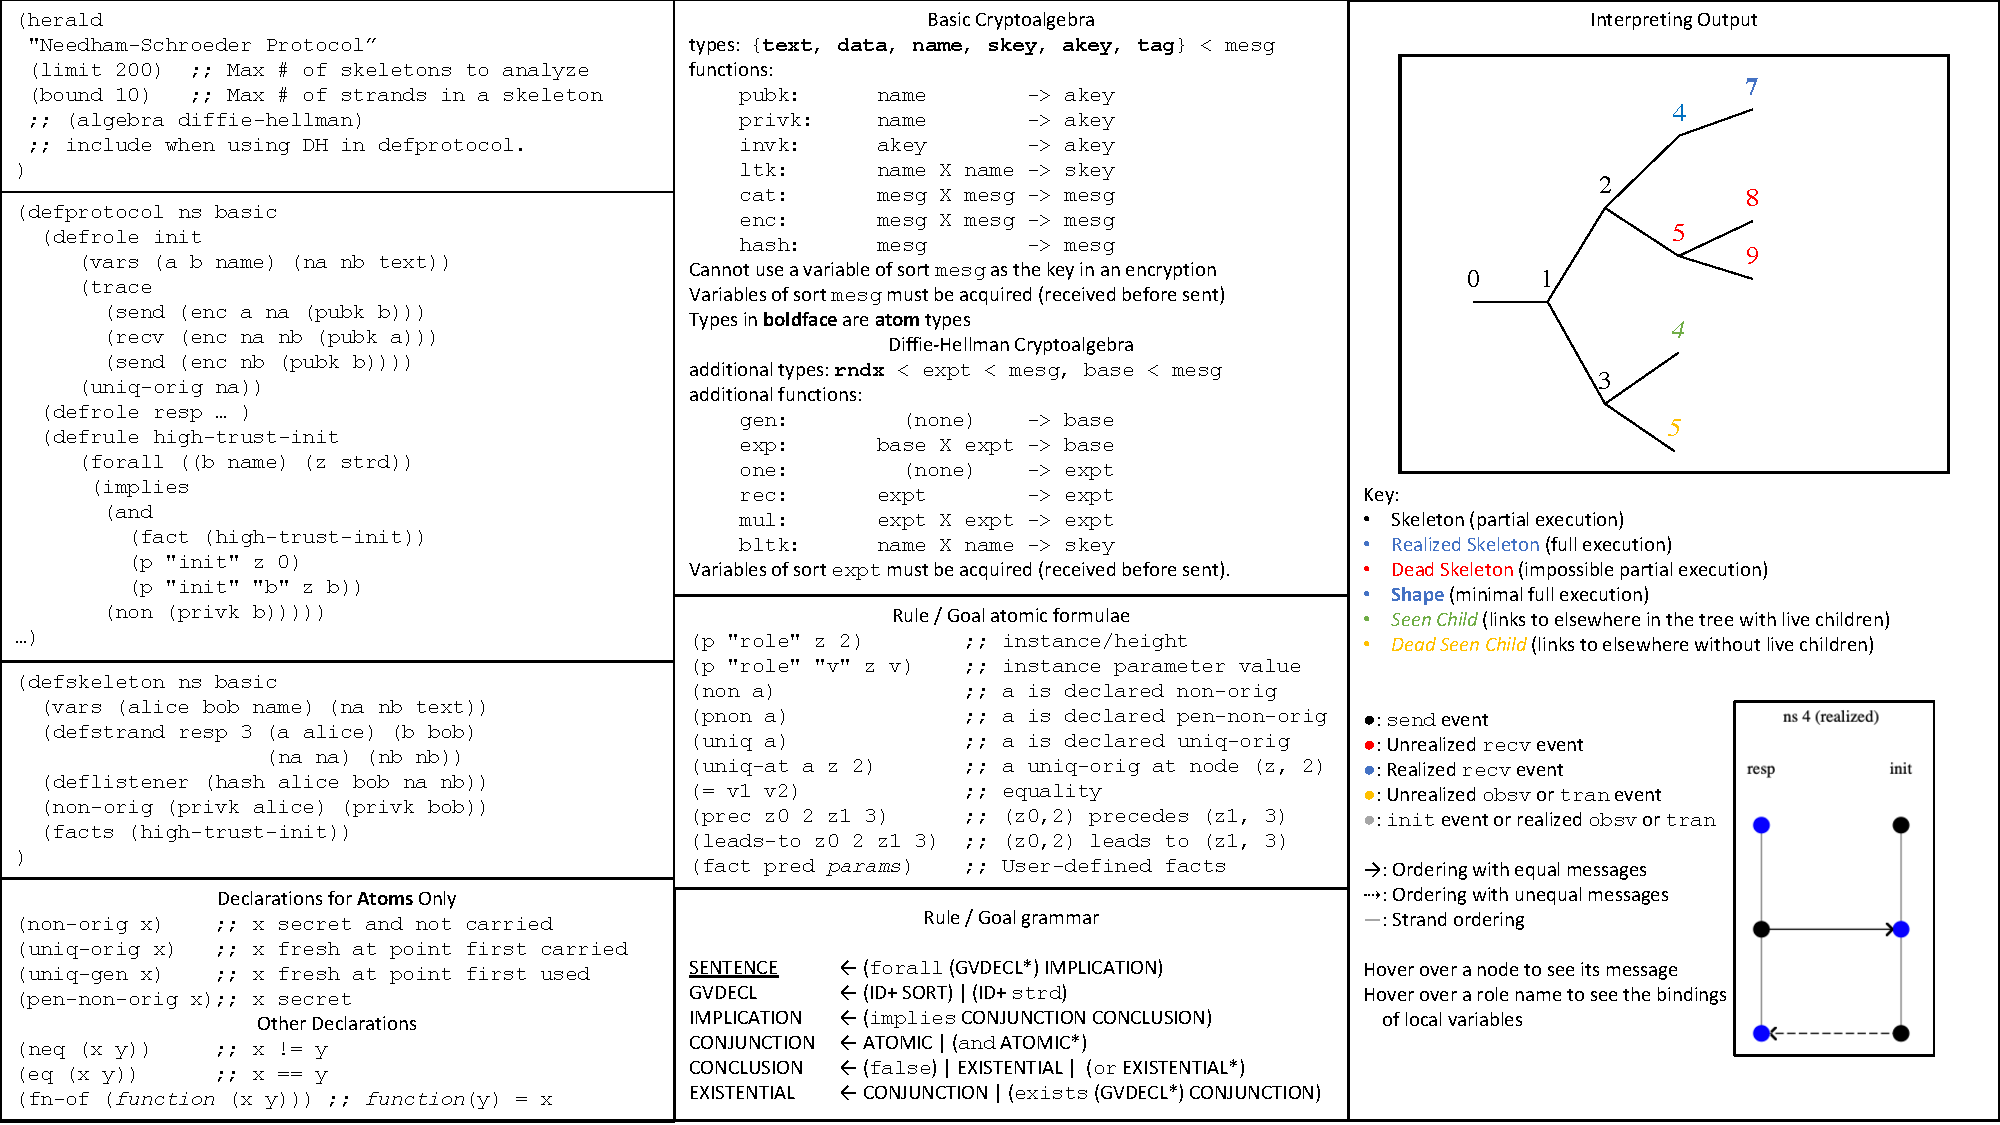
\includepdf[angle=90]{CPSA_cribsheet}

\end{document}

%%% Local Variables:
%%% mode: latex
%%% TeX-master: t
%%% End:
